% Options for packages loaded elsewhere
\PassOptionsToPackage{unicode}{hyperref}
\PassOptionsToPackage{hyphens}{url}
%
\documentclass[
]{article}
\usepackage{amsmath,amssymb}
\usepackage{lmodern}
\usepackage{ifxetex,ifluatex}
\ifnum 0\ifxetex 1\fi\ifluatex 1\fi=0 % if pdftex
  \usepackage[T1]{fontenc}
  \usepackage[utf8]{inputenc}
  \usepackage{textcomp} % provide euro and other symbols
\else % if luatex or xetex
  \usepackage{unicode-math}
  \defaultfontfeatures{Scale=MatchLowercase}
  \defaultfontfeatures[\rmfamily]{Ligatures=TeX,Scale=1}
\fi
% Use upquote if available, for straight quotes in verbatim environments
\IfFileExists{upquote.sty}{\usepackage{upquote}}{}
\IfFileExists{microtype.sty}{% use microtype if available
  \usepackage[]{microtype}
  \UseMicrotypeSet[protrusion]{basicmath} % disable protrusion for tt fonts
}{}
\makeatletter
\@ifundefined{KOMAClassName}{% if non-KOMA class
  \IfFileExists{parskip.sty}{%
    \usepackage{parskip}
  }{% else
    \setlength{\parindent}{0pt}
    \setlength{\parskip}{6pt plus 2pt minus 1pt}}
}{% if KOMA class
  \KOMAoptions{parskip=half}}
\makeatother
\usepackage{xcolor}
\IfFileExists{xurl.sty}{\usepackage{xurl}}{} % add URL line breaks if available
\IfFileExists{bookmark.sty}{\usepackage{bookmark}}{\usepackage{hyperref}}
\hypersetup{
  pdftitle={Scripps's Murrelet Egg Size model},
  pdfauthor={Amelia J. DuVall \& Marcela Todd},
  hidelinks,
  pdfcreator={LaTeX via pandoc}}
\urlstyle{same} % disable monospaced font for URLs
\usepackage[margin=1in]{geometry}
\usepackage{color}
\usepackage{fancyvrb}
\newcommand{\VerbBar}{|}
\newcommand{\VERB}{\Verb[commandchars=\\\{\}]}
\DefineVerbatimEnvironment{Highlighting}{Verbatim}{commandchars=\\\{\}}
% Add ',fontsize=\small' for more characters per line
\usepackage{framed}
\definecolor{shadecolor}{RGB}{248,248,248}
\newenvironment{Shaded}{\begin{snugshade}}{\end{snugshade}}
\newcommand{\AlertTok}[1]{\textcolor[rgb]{0.94,0.16,0.16}{#1}}
\newcommand{\AnnotationTok}[1]{\textcolor[rgb]{0.56,0.35,0.01}{\textbf{\textit{#1}}}}
\newcommand{\AttributeTok}[1]{\textcolor[rgb]{0.77,0.63,0.00}{#1}}
\newcommand{\BaseNTok}[1]{\textcolor[rgb]{0.00,0.00,0.81}{#1}}
\newcommand{\BuiltInTok}[1]{#1}
\newcommand{\CharTok}[1]{\textcolor[rgb]{0.31,0.60,0.02}{#1}}
\newcommand{\CommentTok}[1]{\textcolor[rgb]{0.56,0.35,0.01}{\textit{#1}}}
\newcommand{\CommentVarTok}[1]{\textcolor[rgb]{0.56,0.35,0.01}{\textbf{\textit{#1}}}}
\newcommand{\ConstantTok}[1]{\textcolor[rgb]{0.00,0.00,0.00}{#1}}
\newcommand{\ControlFlowTok}[1]{\textcolor[rgb]{0.13,0.29,0.53}{\textbf{#1}}}
\newcommand{\DataTypeTok}[1]{\textcolor[rgb]{0.13,0.29,0.53}{#1}}
\newcommand{\DecValTok}[1]{\textcolor[rgb]{0.00,0.00,0.81}{#1}}
\newcommand{\DocumentationTok}[1]{\textcolor[rgb]{0.56,0.35,0.01}{\textbf{\textit{#1}}}}
\newcommand{\ErrorTok}[1]{\textcolor[rgb]{0.64,0.00,0.00}{\textbf{#1}}}
\newcommand{\ExtensionTok}[1]{#1}
\newcommand{\FloatTok}[1]{\textcolor[rgb]{0.00,0.00,0.81}{#1}}
\newcommand{\FunctionTok}[1]{\textcolor[rgb]{0.00,0.00,0.00}{#1}}
\newcommand{\ImportTok}[1]{#1}
\newcommand{\InformationTok}[1]{\textcolor[rgb]{0.56,0.35,0.01}{\textbf{\textit{#1}}}}
\newcommand{\KeywordTok}[1]{\textcolor[rgb]{0.13,0.29,0.53}{\textbf{#1}}}
\newcommand{\NormalTok}[1]{#1}
\newcommand{\OperatorTok}[1]{\textcolor[rgb]{0.81,0.36,0.00}{\textbf{#1}}}
\newcommand{\OtherTok}[1]{\textcolor[rgb]{0.56,0.35,0.01}{#1}}
\newcommand{\PreprocessorTok}[1]{\textcolor[rgb]{0.56,0.35,0.01}{\textit{#1}}}
\newcommand{\RegionMarkerTok}[1]{#1}
\newcommand{\SpecialCharTok}[1]{\textcolor[rgb]{0.00,0.00,0.00}{#1}}
\newcommand{\SpecialStringTok}[1]{\textcolor[rgb]{0.31,0.60,0.02}{#1}}
\newcommand{\StringTok}[1]{\textcolor[rgb]{0.31,0.60,0.02}{#1}}
\newcommand{\VariableTok}[1]{\textcolor[rgb]{0.00,0.00,0.00}{#1}}
\newcommand{\VerbatimStringTok}[1]{\textcolor[rgb]{0.31,0.60,0.02}{#1}}
\newcommand{\WarningTok}[1]{\textcolor[rgb]{0.56,0.35,0.01}{\textbf{\textit{#1}}}}
\usepackage{graphicx}
\makeatletter
\def\maxwidth{\ifdim\Gin@nat@width>\linewidth\linewidth\else\Gin@nat@width\fi}
\def\maxheight{\ifdim\Gin@nat@height>\textheight\textheight\else\Gin@nat@height\fi}
\makeatother
% Scale images if necessary, so that they will not overflow the page
% margins by default, and it is still possible to overwrite the defaults
% using explicit options in \includegraphics[width, height, ...]{}
\setkeys{Gin}{width=\maxwidth,height=\maxheight,keepaspectratio}
% Set default figure placement to htbp
\makeatletter
\def\fps@figure{htbp}
\makeatother
\setlength{\emergencystretch}{3em} % prevent overfull lines
\providecommand{\tightlist}{%
  \setlength{\itemsep}{0pt}\setlength{\parskip}{0pt}}
\setcounter{secnumdepth}{-\maxdimen} % remove section numbering
\ifluatex
  \usepackage{selnolig}  % disable illegal ligatures
\fi

\title{Scripps's Murrelet Egg Size model}
\author{Amelia J. DuVall \& Marcela Todd}
\date{4/11/2021}

\begin{document}
\maketitle

This is v.2021-06-04

\hypertarget{introduction}{%
\section{Introduction}\label{introduction}}

This document details steps taken to model Scripps's Murrelet
(\emph{Synthliboramphus scrippsi}) egg size at Santa Barbara Island
within Channel Islands National Park from 2009-2017.

\hypertarget{load-and-format-data}{%
\section{Load and format data}\label{load-and-format-data}}

\begin{Shaded}
\begin{Highlighting}[]
\NormalTok{egg }\OtherTok{\textless{}{-}} \FunctionTok{read.csv}\NormalTok{(}\FunctionTok{here}\NormalTok{(}\StringTok{"data"}\NormalTok{, }\StringTok{"SCMU\_egg\_data.csv"}\NormalTok{)) }
\NormalTok{covars }\OtherTok{\textless{}{-}} \FunctionTok{read.csv}\NormalTok{(}\FunctionTok{here}\NormalTok{(}\StringTok{"data"}\NormalTok{, }\StringTok{"covariates"}\NormalTok{, }\StringTok{"covars.csv"}\NormalTok{))}

\DocumentationTok{\#\# join covariate data with egg data by year}
\NormalTok{SCMUdf }\OtherTok{\textless{}{-}} \FunctionTok{left\_join}\NormalTok{(egg, covars, }\AttributeTok{by =} \StringTok{"Year"}\NormalTok{) }\SpecialCharTok{\%\textgreater{}\%}
  \FunctionTok{filter}\NormalTok{(TrueOrder }\SpecialCharTok{==} \ConstantTok{TRUE}\NormalTok{) }\SpecialCharTok{\%\textgreater{}\%} \CommentTok{\# egg order known only}
  \FunctionTok{select}\NormalTok{(Year, Observer, Plot, Size, EggOrder, ANCHL, BEUTI, NPGO, ONI, PDO, SST) }\SpecialCharTok{\%\textgreater{}\%}
  \FunctionTok{as\_tibble}\NormalTok{()}
\end{Highlighting}
\end{Shaded}

\hypertarget{null-intercept-only-model-with-2-random-effects}{%
\section{Null Intercept-Only Model with 2 random
effects}\label{null-intercept-only-model-with-2-random-effects}}

This model includes observer and plot as random effects, but does not
include any covariates.

\begin{Shaded}
\begin{Highlighting}[]
\DocumentationTok{\#\# run model}
\NormalTok{nm }\OtherTok{\textless{}{-}} \FunctionTok{lmer}\NormalTok{(Size }\SpecialCharTok{\textasciitilde{}} \DecValTok{1} \SpecialCharTok{+}\NormalTok{ (}\DecValTok{1} \SpecialCharTok{|}\NormalTok{ Observer) }\SpecialCharTok{+}\NormalTok{ (}\DecValTok{1} \SpecialCharTok{|}\NormalTok{ Plot), }\AttributeTok{data =}\NormalTok{ SCMUdf, }\AttributeTok{REML =} \ConstantTok{TRUE}\NormalTok{)}

\DocumentationTok{\#\# look at model output and estimates}
\FunctionTok{sumary}\NormalTok{(nm)}
\end{Highlighting}
\end{Shaded}

\begin{verbatim}
## Fixed Effects:
## coef.est  coef.se 
##  1884.29    12.20 
## 
## Random Effects:
##  Groups   Name        Std.Dev.
##  Observer (Intercept)  17.22  
##  Plot     (Intercept)  24.49  
##  Residual             111.96  
## ---
## number of obs: 753, groups: Observer, 27; Plot, 8
## AIC = 9263.1, DIC = 9268.5
## deviance = 9261.8
\end{verbatim}

\begin{Shaded}
\begin{Highlighting}[]
\FunctionTok{coef}\NormalTok{(nm) }\CommentTok{\# these are the coefficients}
\end{Highlighting}
\end{Shaded}

\begin{verbatim}
## $Observer
##     (Intercept)
## AAY    1899.553
## AJB    1880.127
## AJD    1895.666
## AML    1886.089
## CAC    1876.699
## CEH    1880.914
## CEK    1880.307
## CLE    1879.914
## DLW    1874.348
## EWW    1891.898
## GRK    1882.978
## JAH    1902.680
## KMR    1885.299
## KWB    1880.009
## LAH    1883.315
## MEJ    1878.435
## MGB    1886.816
## NAG    1869.396
## PTL    1876.981
## RER    1893.489
## REW    1881.330
## SAA    1887.456
## SFC    1885.064
## SJK    1893.394
## SKT    1862.709
## SLA    1884.647
## SMC    1896.380
## 
## $Plot
##      (Intercept)
## APNC    1905.622
## BH      1898.588
## BT      1850.797
## CC      1903.414
## DO      1885.298
## ESC     1882.827
## LC      1873.535
## WC      1874.258
## 
## attr(,"class")
## [1] "coef.mer"
\end{verbatim}

\begin{Shaded}
\begin{Highlighting}[]
\FunctionTok{ranef}\NormalTok{(nm) }\CommentTok{\# these are the random effects}
\end{Highlighting}
\end{Shaded}

\begin{verbatim}
## $Observer
##     (Intercept)
## AAY  15.2610062
## AJB  -4.1654786
## AJD  11.3739567
## AML   1.7970244
## CAC  -7.5934214
## CEH  -3.3784652
## CEK  -3.9853109
## CLE  -4.3779272
## DLW  -9.9445690
## EWW   7.6052536
## GRK  -1.3144290
## JAH  18.3876524
## KMR   1.0067101
## KWB  -4.2835217
## LAH  -0.9770916
## MEJ  -5.8572070
## MGB   2.5241208
## NAG -14.8959509
## PTL  -7.3117215
## RER   9.1963408
## REW  -2.9625711
## SAA   3.1632622
## SFC   0.7713125
## SJK   9.1015277
## SKT -21.5831481
## SLA   0.3551011
## SMC  12.0875447
## 
## $Plot
##      (Intercept)
## APNC   21.329246
## BH     14.295406
## BT    -33.494909
## CC     19.121674
## DO      1.005254
## ESC    -1.464948
## LC    -10.757089
## WC    -10.034635
## 
## with conditional variances for "Observer" "Plot"
\end{verbatim}

\begin{Shaded}
\begin{Highlighting}[]
\DocumentationTok{\#\# you can store the model results to objects}
\NormalTok{obs.ranef }\OtherTok{\textless{}{-}} \FunctionTok{ranef}\NormalTok{(nm)}\SpecialCharTok{$}\NormalTok{Observer }
\NormalTok{plot.ranef }\OtherTok{\textless{}{-}} \FunctionTok{ranef}\NormalTok{(nm)}\SpecialCharTok{$}\NormalTok{Plot}
\DocumentationTok{\#\# the mean of these values should be close to 0}
\FunctionTok{mean}\NormalTok{(obs.ranef[[}\DecValTok{1}\NormalTok{]])}
\end{Highlighting}
\end{Shaded}

\begin{verbatim}
## [1] 3.494283e-13
\end{verbatim}

\begin{Shaded}
\begin{Highlighting}[]
\FunctionTok{mean}\NormalTok{(plot.ranef[[}\DecValTok{1}\NormalTok{]])}
\end{Highlighting}
\end{Shaded}

\begin{verbatim}
## [1] -7.280149e-12
\end{verbatim}

\begin{Shaded}
\begin{Highlighting}[]
\DocumentationTok{\#\# quick model diagnostics}
\DocumentationTok{\#\# extract predicted values and plot}
\NormalTok{preds }\OtherTok{\textless{}{-}} \FunctionTok{predict}\NormalTok{(nm) }
\FunctionTok{ggplot}\NormalTok{() }\SpecialCharTok{+} 
  \FunctionTok{geom\_histogram}\NormalTok{(}\AttributeTok{mapping =} \FunctionTok{aes}\NormalTok{(preds)) }\SpecialCharTok{+} 
  \FunctionTok{theme\_minimal}\NormalTok{() }
\end{Highlighting}
\end{Shaded}

\begin{verbatim}
## `stat_bin()` using `bins = 30`. Pick better value with `binwidth`.
\end{verbatim}

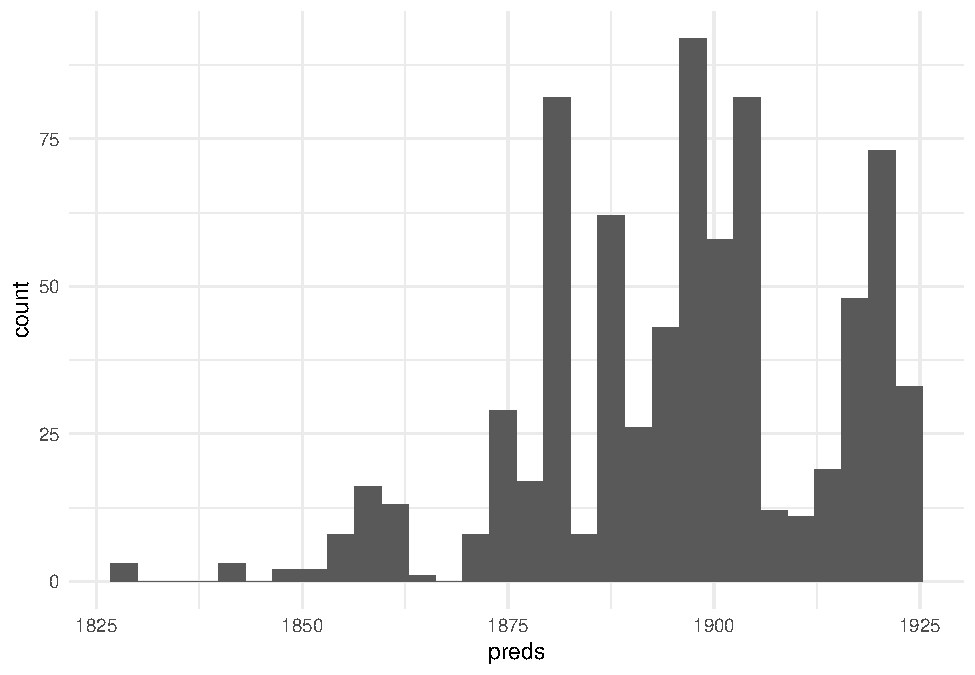
\includegraphics{SCMU_egg_model_files/figure-latex/null_model-1.pdf}

\begin{Shaded}
\begin{Highlighting}[]
\CommentTok{\# we want these to look normally distributed}

\DocumentationTok{\#\# extract residuals and plot}
\NormalTok{resids }\OtherTok{\textless{}{-}} \FunctionTok{residuals}\NormalTok{(nm) }
\FunctionTok{ggplot}\NormalTok{() }\SpecialCharTok{+} 
  \FunctionTok{geom\_histogram}\NormalTok{(}\AttributeTok{mapping =} \FunctionTok{aes}\NormalTok{(resids)) }\SpecialCharTok{+} 
  \FunctionTok{theme\_minimal}\NormalTok{()}
\end{Highlighting}
\end{Shaded}

\begin{verbatim}
## `stat_bin()` using `bins = 30`. Pick better value with `binwidth`.
\end{verbatim}

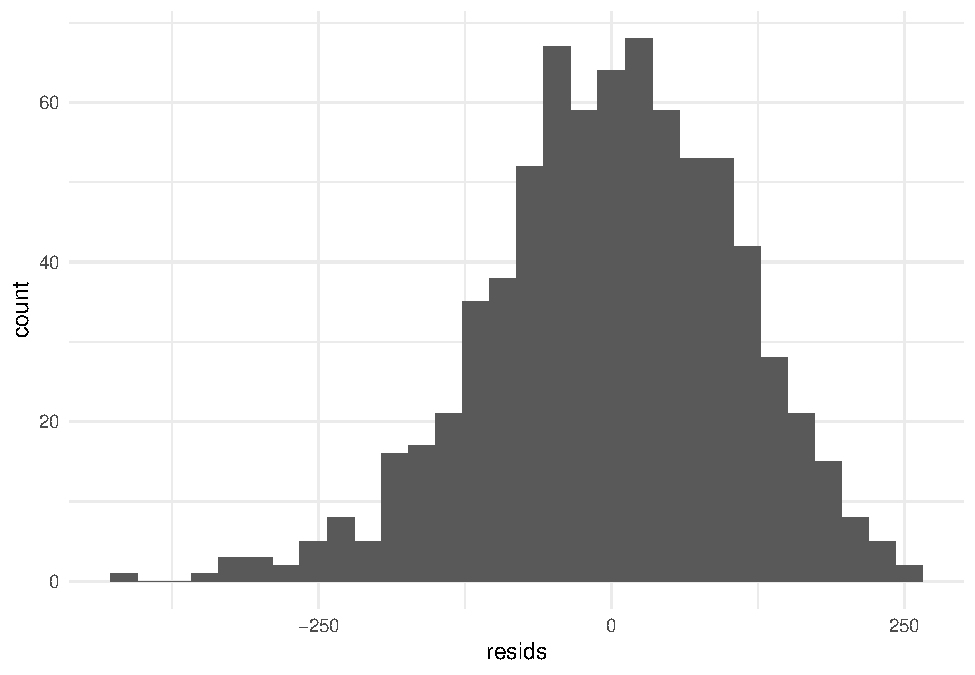
\includegraphics{SCMU_egg_model_files/figure-latex/null_model-2.pdf}

\begin{Shaded}
\begin{Highlighting}[]
\CommentTok{\# we want these to look normally distributed}

\CommentTok{\# qq resids}
\FunctionTok{qqnorm}\NormalTok{(resids, }\AttributeTok{main =} \StringTok{"QQ plot (residuals)"}\NormalTok{, }\AttributeTok{las =} \DecValTok{1}\NormalTok{, }\AttributeTok{pch =} \DecValTok{16}\NormalTok{)}
\FunctionTok{qqline}\NormalTok{(resids)}
\end{Highlighting}
\end{Shaded}

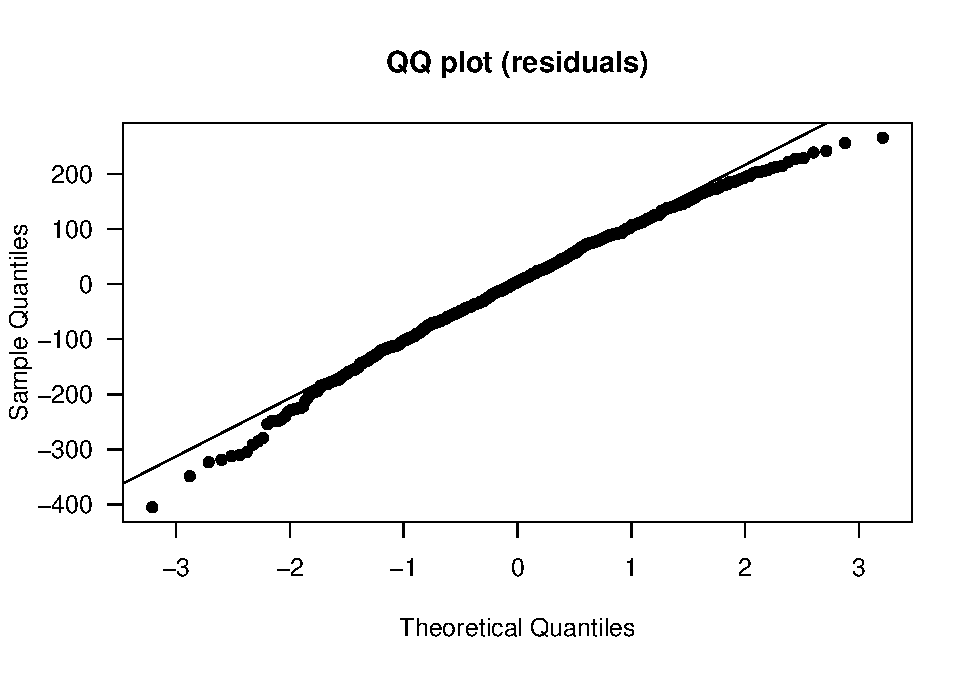
\includegraphics{SCMU_egg_model_files/figure-latex/null_model-3.pdf}

\begin{Shaded}
\begin{Highlighting}[]
\DocumentationTok{\#\# plot residuals versus fitted values}
\NormalTok{yh }\OtherTok{\textless{}{-}} \FunctionTok{fitted}\NormalTok{(nm)}
\FunctionTok{plot}\NormalTok{(yh, resids, }\AttributeTok{las =} \DecValTok{1}\NormalTok{, }\AttributeTok{pch =} \DecValTok{16}\NormalTok{,}
     \AttributeTok{xlab =} \StringTok{"Fitted"}\NormalTok{, }\AttributeTok{ylab =} \StringTok{"Residuals"}\NormalTok{,}
     \AttributeTok{main =} \StringTok{"Residuals vs fitted"}\NormalTok{)}
\FunctionTok{abline}\NormalTok{(}\AttributeTok{h=}\DecValTok{0}\NormalTok{, }\AttributeTok{lty =} \StringTok{"dashed"}\NormalTok{)}
\end{Highlighting}
\end{Shaded}

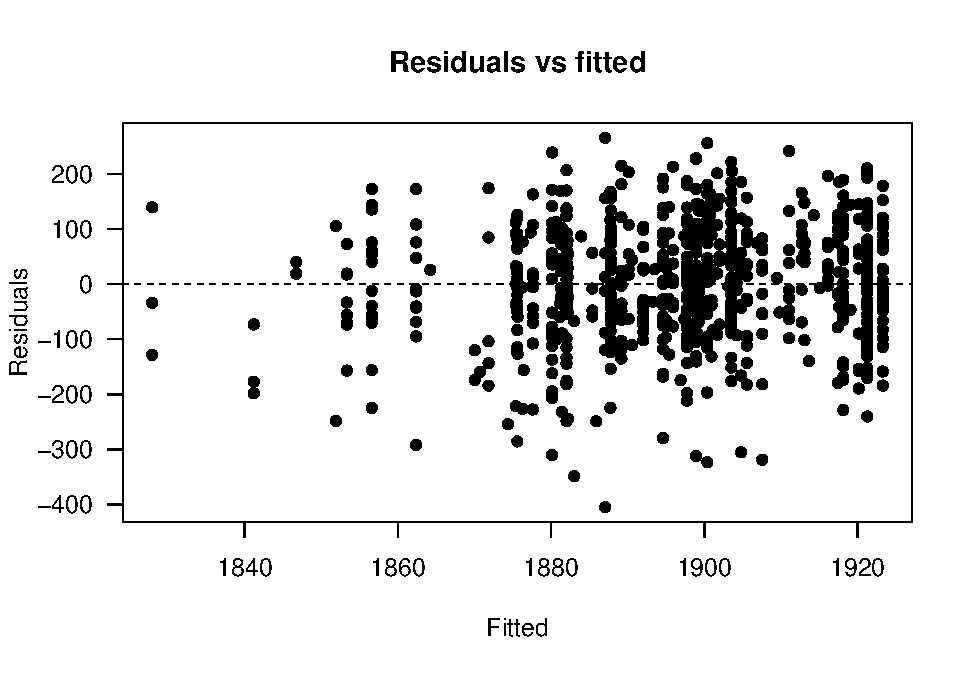
\includegraphics{SCMU_egg_model_files/figure-latex/null_model-4.pdf}

\hypertarget{remove-correlated-predictos-find-global-model}{%
\section{Remove Correlated Predictos \& Find Global
Model}\label{remove-correlated-predictos-find-global-model}}

\begin{Shaded}
\begin{Highlighting}[]
\DocumentationTok{\#\# create data frame specifying predictors to include}
\NormalTok{predictors }\OtherTok{\textless{}{-}} \FunctionTok{as.data.frame}\NormalTok{(}\FunctionTok{matrix}\NormalTok{(}\FunctionTok{c}\NormalTok{(}\ConstantTok{FALSE}\NormalTok{, }\ConstantTok{TRUE}\NormalTok{), }\DecValTok{2}\NormalTok{, }\DecValTok{7}\NormalTok{)) }\CommentTok{\# 7 potential predictors (includes EggOrder)}

\DocumentationTok{\#\# add column names}
\NormalTok{cov\_names }\OtherTok{\textless{}{-}} \FunctionTok{colnames}\NormalTok{(predictors) }\OtherTok{\textless{}{-}} \FunctionTok{colnames}\NormalTok{(SCMUdf[,}\DecValTok{5}\SpecialCharTok{:}\DecValTok{11}\NormalTok{])}

\DocumentationTok{\#\# create set of all possible combinations}
\NormalTok{full\_set }\OtherTok{\textless{}{-}} \FunctionTok{expand.grid}\NormalTok{(predictors) }\CommentTok{\# 128 combinations}

\DocumentationTok{\#\# select models with correlated predictors (see SCMU\_egg\_covariates.Rmd)}
\NormalTok{ii }\OtherTok{\textless{}{-}} \FunctionTok{which}\NormalTok{(full\_set}\SpecialCharTok{$}\NormalTok{ANCHL }\SpecialCharTok{+}\NormalTok{ full\_set}\SpecialCharTok{$}\NormalTok{NPGO }\SpecialCharTok{==} \DecValTok{2} \SpecialCharTok{|}
\NormalTok{              full\_set}\SpecialCharTok{$}\NormalTok{ANCHL }\SpecialCharTok{+}\NormalTok{ full\_set}\SpecialCharTok{$}\NormalTok{ONI }\SpecialCharTok{==} \DecValTok{2} \SpecialCharTok{|}
\NormalTok{              full\_set}\SpecialCharTok{$}\NormalTok{ANCHL }\SpecialCharTok{+}\NormalTok{ full\_set}\SpecialCharTok{$}\NormalTok{PDO }\SpecialCharTok{==} \DecValTok{2} \SpecialCharTok{|}
\NormalTok{              full\_set}\SpecialCharTok{$}\NormalTok{BEUTI }\SpecialCharTok{+}\NormalTok{ full\_set}\SpecialCharTok{$}\NormalTok{ONI }\SpecialCharTok{==} \DecValTok{2} \SpecialCharTok{|}
\NormalTok{              full\_set}\SpecialCharTok{$}\NormalTok{BEUTI }\SpecialCharTok{+}\NormalTok{ full\_set}\SpecialCharTok{$}\NormalTok{PDO }\SpecialCharTok{==} \DecValTok{2} \SpecialCharTok{|}
\NormalTok{              full\_set}\SpecialCharTok{$}\NormalTok{NPGO }\SpecialCharTok{+}\NormalTok{ full\_set}\SpecialCharTok{$}\NormalTok{PDO }\SpecialCharTok{==} \DecValTok{2} \SpecialCharTok{|}
\NormalTok{              full\_set}\SpecialCharTok{$}\NormalTok{NPGO }\SpecialCharTok{+}\NormalTok{ full\_set}\SpecialCharTok{$}\NormalTok{SST }\SpecialCharTok{==} \DecValTok{2} \SpecialCharTok{|}
\NormalTok{              full\_set}\SpecialCharTok{$}\NormalTok{ONI }\SpecialCharTok{+}\NormalTok{ full\_set}\SpecialCharTok{$}\NormalTok{PDO }\SpecialCharTok{==} \DecValTok{2}\NormalTok{) }\CommentTok{\# 98 models}

\DocumentationTok{\#\# create reduced set of models and convert to a matrix for easier indexing}
\NormalTok{use\_set }\OtherTok{\textless{}{-}} \FunctionTok{as.matrix}\NormalTok{(full\_set[}\SpecialCharTok{{-}}\NormalTok{ii,]) }

\DocumentationTok{\#\# number of models in set}
\NormalTok{(n\_mods }\OtherTok{\textless{}{-}} \FunctionTok{nrow}\NormalTok{(use\_set)) }\CommentTok{\# 30 models out of potential 128}
\end{Highlighting}
\end{Shaded}

\begin{verbatim}
## [1] 30
\end{verbatim}

\begin{Shaded}
\begin{Highlighting}[]
\DocumentationTok{\#\# find max number of predictors in a model}
\FunctionTok{rowSums}\NormalTok{(use\_set) }\CommentTok{\# only one model with 4 predictors (72)}
\end{Highlighting}
\end{Shaded}

\begin{verbatim}
##  1  2  3  4  5  6  7  8  9 10 13 14 17 18 25 26 33 34 65 66 67 68 69 70 71 72 
##  0  1  1  2  1  2  2  3  1  2  2  3  1  2  2  3  1  2  1  2  2  3  2  3  3  4 
## 81 82 97 98 
##  2  3  2  3
\end{verbatim}

\begin{Shaded}
\begin{Highlighting}[]
\DocumentationTok{\#\# which predictors are included in this model?}
\NormalTok{cov\_names[use\_set[}\DecValTok{26}\NormalTok{,]] }\CommentTok{\# "EggOrder" "ANCHL"    "BEUTI"    "SST"  }
\end{Highlighting}
\end{Shaded}

\begin{verbatim}
## [1] "EggOrder" "ANCHL"    "BEUTI"    "SST"
\end{verbatim}

\hypertarget{likelihood-ratio-tests}{%
\section{Likelihood Ratio Tests}\label{likelihood-ratio-tests}}

We used LRTs using the global model to test the support for inclusion of
random effects (Plot, Observer). There are NAs in the observer data from
2015. These NAs need to be removed prior to completing LRT tests. See
\url{https://cran.r-project.org/web/packages/RLRsim/RLRsim.pdf} for
info.

\begin{Shaded}
\begin{Highlighting}[]
\NormalTok{SCMUdf2 }\OtherTok{\textless{}{-}}\NormalTok{ SCMUdf[}\SpecialCharTok{{-}}\FunctionTok{c}\NormalTok{(}\FunctionTok{which}\NormalTok{(}\FunctionTok{is.na}\NormalTok{(SCMUdf}\SpecialCharTok{$}\NormalTok{Observer}\SpecialCharTok{==}\ConstantTok{TRUE}\NormalTok{))),]}

\DocumentationTok{\#\# global model}
\NormalTok{bm\_both }\OtherTok{\textless{}{-}} \FunctionTok{lmer}\NormalTok{(Size }\SpecialCharTok{\textasciitilde{}}\NormalTok{ EggOrder }\SpecialCharTok{+}\NormalTok{ ANCHL }\SpecialCharTok{+}\NormalTok{ BEUTI }\SpecialCharTok{+}\NormalTok{ SST }\SpecialCharTok{+}\NormalTok{ (}\DecValTok{1} \SpecialCharTok{|}\NormalTok{ Observer) }\SpecialCharTok{+}\NormalTok{ (}\DecValTok{1} \SpecialCharTok{|}\NormalTok{ Plot), }\AttributeTok{data =}\NormalTok{ SCMUdf2, }\AttributeTok{REML =} \ConstantTok{FALSE}\NormalTok{)}

\DocumentationTok{\#\# run model with plot RE only}
\NormalTok{bm\_plot }\OtherTok{\textless{}{-}} \FunctionTok{lmer}\NormalTok{(Size }\SpecialCharTok{\textasciitilde{}}\NormalTok{ EggOrder }\SpecialCharTok{+}\NormalTok{ ANCHL }\SpecialCharTok{+}\NormalTok{ BEUTI }\SpecialCharTok{+}\NormalTok{ SST }\SpecialCharTok{+}\NormalTok{ (}\DecValTok{1} \SpecialCharTok{|}\NormalTok{ Plot), }\AttributeTok{data =}\NormalTok{ SCMUdf2, }\AttributeTok{REML =} \ConstantTok{FALSE}\NormalTok{)}

\DocumentationTok{\#\# run model with obs RE only}
\NormalTok{bm\_obs }\OtherTok{\textless{}{-}} \FunctionTok{lmer}\NormalTok{(Size }\SpecialCharTok{\textasciitilde{}}\NormalTok{ EggOrder }\SpecialCharTok{+}\NormalTok{ ANCHL }\SpecialCharTok{+}\NormalTok{ BEUTI }\SpecialCharTok{+}\NormalTok{ SST }\SpecialCharTok{+}\NormalTok{ (}\DecValTok{1} \SpecialCharTok{|}\NormalTok{ Observer), }\AttributeTok{data =}\NormalTok{ SCMUdf2, }\AttributeTok{REML =} \ConstantTok{FALSE}\NormalTok{)}

\DocumentationTok{\#\# Exact RLRT test}
\CommentTok{\# m is the reduced model containing only the RE to be tested (the random effect set to zero under the null hypothesis). mA and Mo are the models under the alternative and the null, respectively. }

\CommentTok{\# observer set to zero under the null hypothesis}
\FunctionTok{exactRLRT}\NormalTok{(}\AttributeTok{m =}\NormalTok{ bm\_obs, }\AttributeTok{mA =}\NormalTok{ bm\_both, }\AttributeTok{m0 =}\NormalTok{ bm\_plot, }\AttributeTok{seed =} \DecValTok{16}\NormalTok{)}
\end{Highlighting}
\end{Shaded}

\begin{verbatim}
## Using restricted likelihood evaluated at ML estimators.
\end{verbatim}

\begin{verbatim}
## Refit with method="REML" for exact results.
\end{verbatim}

\begin{verbatim}
## 
##  simulated finite sample distribution of RLRT.
##  
##  (p-value based on 10000 simulated values)
## 
## data:  
## RLRT = 1.2984, p-value = 0.0946
\end{verbatim}

\begin{Shaded}
\begin{Highlighting}[]
\CommentTok{\# plot set to zero under the null hypothesis }
\FunctionTok{exactRLRT}\NormalTok{(}\AttributeTok{m =}\NormalTok{ bm\_plot, }\AttributeTok{mA =}\NormalTok{ bm\_both, }\AttributeTok{m0 =}\NormalTok{ bm\_obs, }\AttributeTok{seed =} \DecValTok{16}\NormalTok{)}
\end{Highlighting}
\end{Shaded}

\begin{verbatim}
## Using restricted likelihood evaluated at ML estimators.
## Refit with method="REML" for exact results.
\end{verbatim}

\begin{verbatim}
## 
##  simulated finite sample distribution of RLRT.
##  
##  (p-value based on 10000 simulated values)
## 
## data:  
## RLRT = 3.8766, p-value = 0.0138
\end{verbatim}

\hypertarget{model-diagnostics}{%
\section{Model Diagnostics}\label{model-diagnostics}}

These diagnostics are done for the global model.

\begin{Shaded}
\begin{Highlighting}[]
\DocumentationTok{\#\# run global model}
\NormalTok{global\_mod }\OtherTok{\textless{}{-}} \FunctionTok{lmer}\NormalTok{(Size }\SpecialCharTok{\textasciitilde{}}\NormalTok{ EggOrder }\SpecialCharTok{+}\NormalTok{ ANCHL }\SpecialCharTok{+}\NormalTok{ BEUTI }\SpecialCharTok{+}\NormalTok{ SST }\SpecialCharTok{+}\NormalTok{ (}\DecValTok{1} \SpecialCharTok{|}\NormalTok{ Plot), }\AttributeTok{data =}\NormalTok{ SCMUdf, }\AttributeTok{REML =} \ConstantTok{TRUE}\NormalTok{)}
\end{Highlighting}
\end{Shaded}

\hypertarget{residualsfitted-plots}{%
\subsection{Residuals/Fitted Plots}\label{residualsfitted-plots}}

\hypertarget{histogram-of-predicted-values}{%
\subsubsection{Histogram of Predicted
Values}\label{histogram-of-predicted-values}}

\begin{Shaded}
\begin{Highlighting}[]
\DocumentationTok{\#\# extract predicted values and plot}
\NormalTok{preds }\OtherTok{\textless{}{-}} \FunctionTok{predict}\NormalTok{(global\_mod)}
\FunctionTok{ggplot}\NormalTok{() }\SpecialCharTok{+} 
  \FunctionTok{geom\_histogram}\NormalTok{(}\AttributeTok{mapping =} \FunctionTok{aes}\NormalTok{(preds), }\AttributeTok{bins =} \DecValTok{20}\NormalTok{) }\SpecialCharTok{+} \CommentTok{\# set bins }
  \FunctionTok{theme\_minimal}\NormalTok{()}
\end{Highlighting}
\end{Shaded}

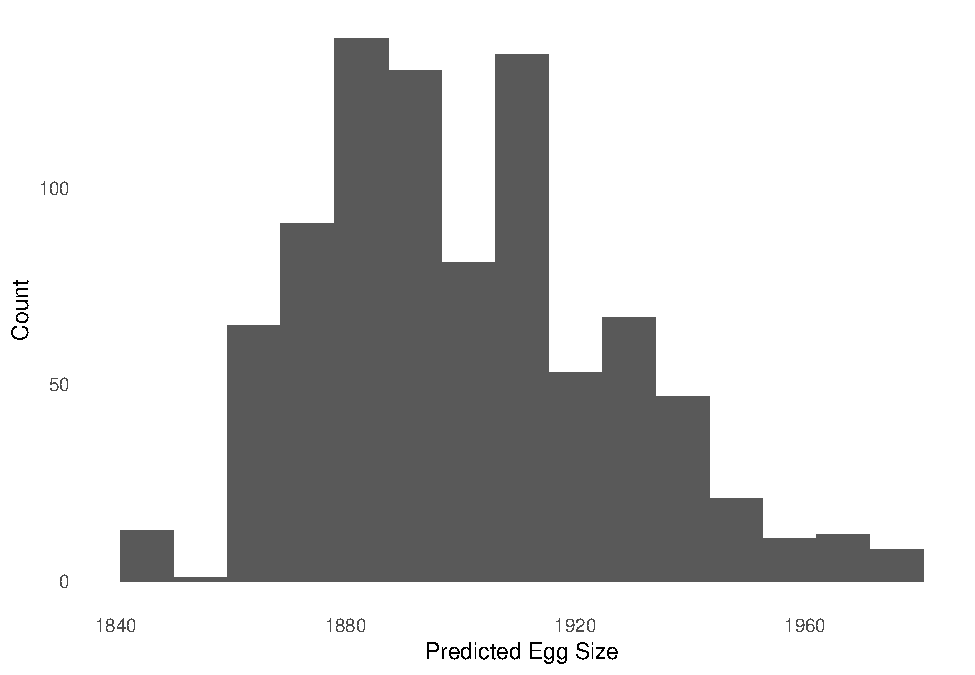
\includegraphics{SCMU_egg_model_files/figure-latex/d1-1.pdf} Since we
assumed our data are normal, we want to see an approximately normal
distribution of predicted values.

\hypertarget{histogram-of-residuals}{%
\subsubsection{Histogram of Residuals}\label{histogram-of-residuals}}

\begin{Shaded}
\begin{Highlighting}[]
\DocumentationTok{\#\# extract residuals and plot}
\NormalTok{resids }\OtherTok{\textless{}{-}} \FunctionTok{residuals}\NormalTok{(global\_mod)}
\FunctionTok{ggplot}\NormalTok{() }\SpecialCharTok{+} 
  \FunctionTok{geom\_histogram}\NormalTok{(}\AttributeTok{mapping =} \FunctionTok{aes}\NormalTok{(resids), }\AttributeTok{bins =} \DecValTok{20}\NormalTok{) }\SpecialCharTok{+} 
  \FunctionTok{theme\_minimal}\NormalTok{()}
\end{Highlighting}
\end{Shaded}

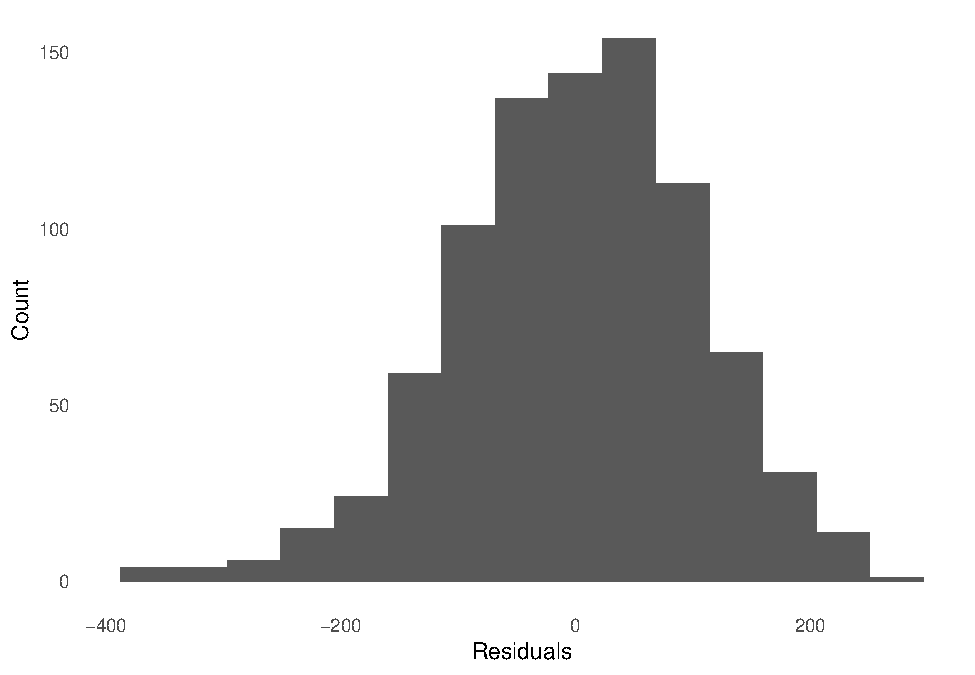
\includegraphics{SCMU_egg_model_files/figure-latex/d2-1.pdf} Since we
assumed our data are normal, we want to see an approximately normal
distribution of residuals (differences between observed and predicted
values of data).

\hypertarget{model-coefficients}{%
\subsubsection{Model Coefficients}\label{model-coefficients}}

\begin{Shaded}
\begin{Highlighting}[]
\DocumentationTok{\#\# extract coeffs and random effects}
\FunctionTok{coef}\NormalTok{(global\_mod) }\CommentTok{\# this include fixed and random effects}
\end{Highlighting}
\end{Shaded}

\begin{verbatim}
## $Plot
##      (Intercept) EggOrderEgg2    ANCHL    BEUTI      SST
## APNC    1895.298     32.93263 4.806984 -11.3738 7.697737
## BH      1899.198     32.93263 4.806984 -11.3738 7.697737
## BT      1854.966     32.93263 4.806984 -11.3738 7.697737
## CC      1902.741     32.93263 4.806984 -11.3738 7.697737
## DO      1883.361     32.93263 4.806984 -11.3738 7.697737
## ESC     1883.376     32.93263 4.806984 -11.3738 7.697737
## LC      1876.946     32.93263 4.806984 -11.3738 7.697737
## WC      1874.641     32.93263 4.806984 -11.3738 7.697737
## 
## attr(,"class")
## [1] "coef.mer"
\end{verbatim}

\begin{Shaded}
\begin{Highlighting}[]
\NormalTok{ranef\_pl }\OtherTok{\textless{}{-}} \FunctionTok{ranef}\NormalTok{(global\_mod)}\SpecialCharTok{$}\NormalTok{Plot }\CommentTok{\# plot random effect only}

\DocumentationTok{\#\# look at data going into random effects}
\FunctionTok{table}\NormalTok{(SCMUdf}\SpecialCharTok{$}\NormalTok{Plot)}
\end{Highlighting}
\end{Shaded}

\begin{verbatim}
## 
## APNC   BH   BT   CC   DO  ESC   LC   WC 
##  115   31   16  275  192    1  240    4
\end{verbatim}

We can extract our model coefficients (for fixed and random effects) and
look at them.

\hypertarget{q-q-plots}{%
\subsubsection{Q-Q Plots}\label{q-q-plots}}

\begin{Shaded}
\begin{Highlighting}[]
\CommentTok{\# qq resids}
\FunctionTok{qqnorm}\NormalTok{(resids, }\AttributeTok{main =} \StringTok{"QQ plot (residuals)"}\NormalTok{, }\AttributeTok{las =} \DecValTok{1}\NormalTok{, }\AttributeTok{pch =} \DecValTok{16}\NormalTok{)}
\FunctionTok{qqline}\NormalTok{(resids)}
\end{Highlighting}
\end{Shaded}

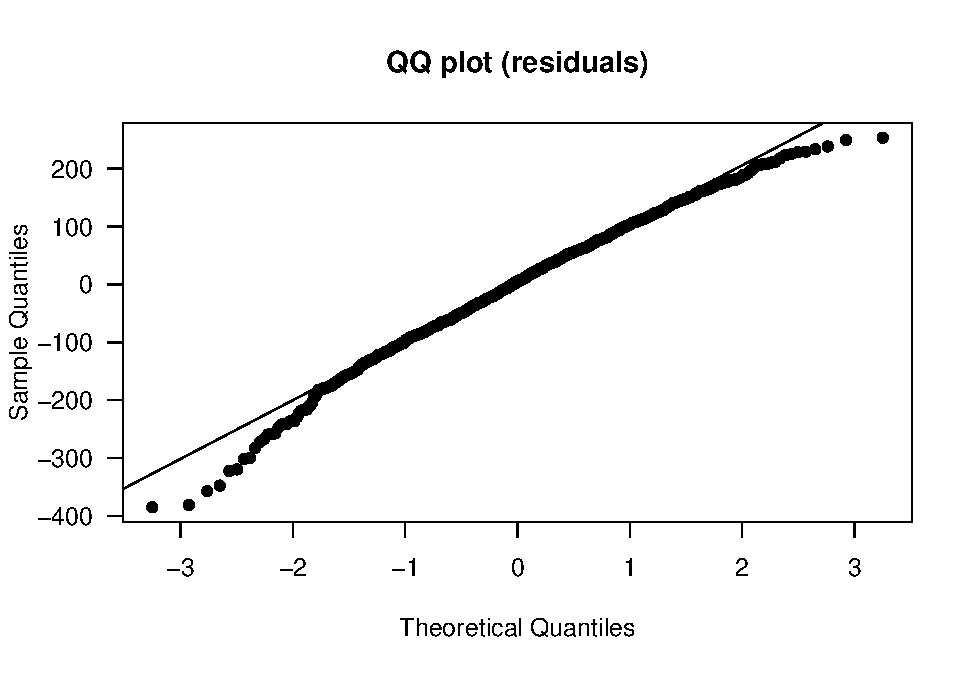
\includegraphics{SCMU_egg_model_files/figure-latex/d4-1.pdf}

\begin{Shaded}
\begin{Highlighting}[]
\CommentTok{\# qq Plot RE}
\FunctionTok{qqnorm}\NormalTok{(}\FunctionTok{unlist}\NormalTok{(ranef\_pl), }\AttributeTok{main =} \StringTok{"QQ plot (Plot RE)"}\NormalTok{, }\AttributeTok{las =} \DecValTok{1}\NormalTok{, }\AttributeTok{pch =} \DecValTok{16}\NormalTok{)}
\FunctionTok{qqline}\NormalTok{(}\FunctionTok{unlist}\NormalTok{(ranef\_pl))}
\end{Highlighting}
\end{Shaded}

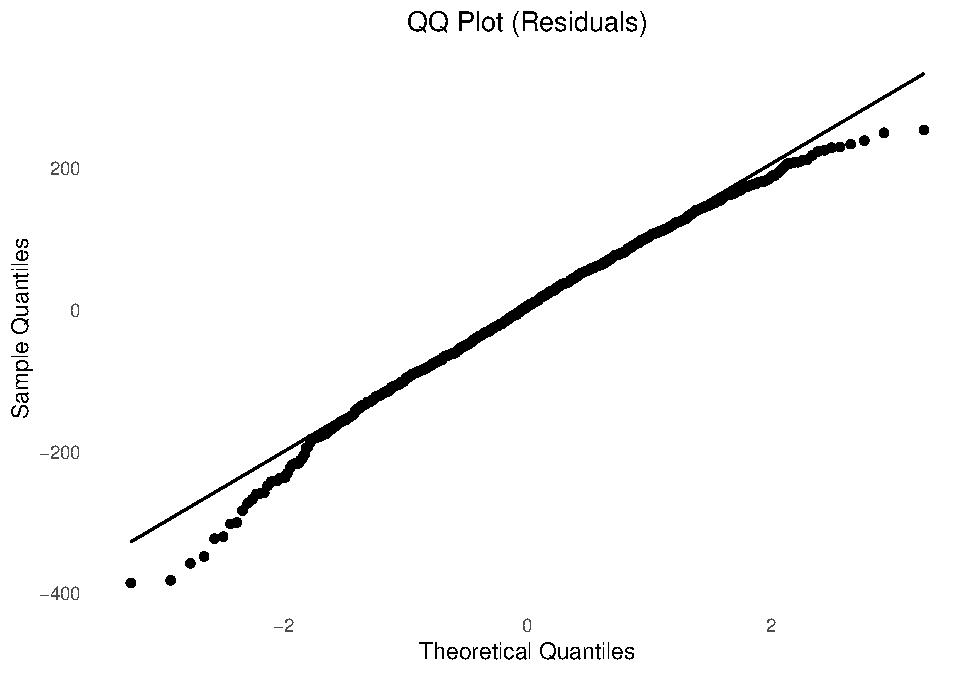
\includegraphics{SCMU_egg_model_files/figure-latex/d4-2.pdf} We want our
points to fall approximately on the diagonal lines.

\hypertarget{fitted-v-residuals}{%
\subsubsection{Fitted v Residuals}\label{fitted-v-residuals}}

\begin{Shaded}
\begin{Highlighting}[]
\DocumentationTok{\#\# plot residuals versus fitted values}
\NormalTok{yh }\OtherTok{\textless{}{-}} \FunctionTok{fitted}\NormalTok{(global\_mod)}
\FunctionTok{plot}\NormalTok{(yh, resids, }\AttributeTok{las =} \DecValTok{1}\NormalTok{, }\AttributeTok{pch =} \DecValTok{16}\NormalTok{,}
     \AttributeTok{xlab =} \StringTok{"Fitted"}\NormalTok{, }\AttributeTok{ylab =} \StringTok{"Residuals"}\NormalTok{,}
     \AttributeTok{main =} \StringTok{"Residuals vs fitted"}\NormalTok{)}
\FunctionTok{abline}\NormalTok{(}\AttributeTok{h=}\DecValTok{0}\NormalTok{, }\AttributeTok{lty =} \StringTok{"dashed"}\NormalTok{)}
\end{Highlighting}
\end{Shaded}

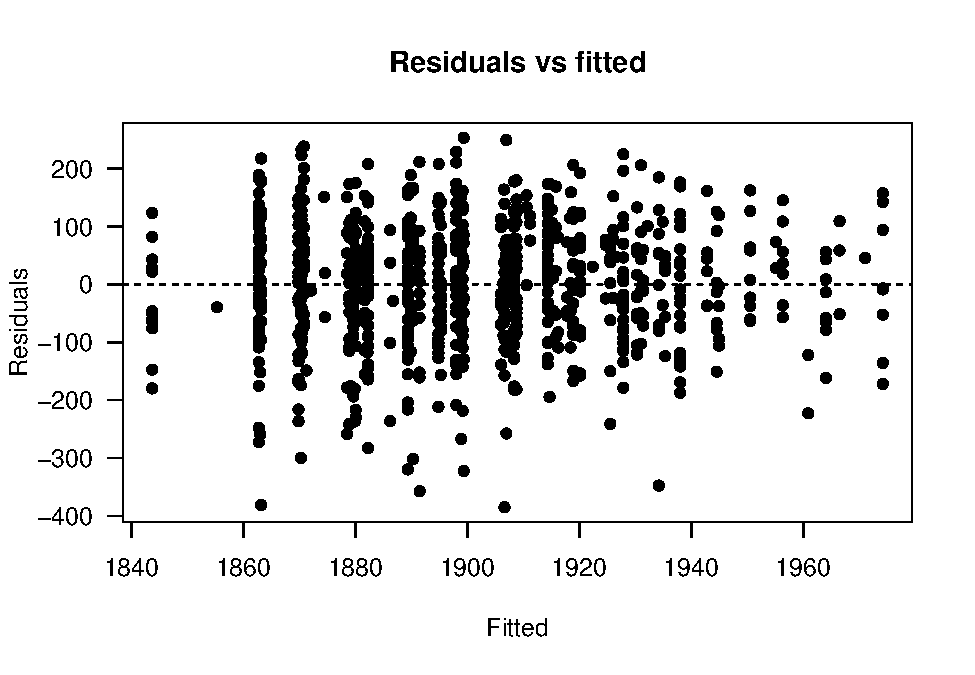
\includegraphics{SCMU_egg_model_files/figure-latex/d5-1.pdf} We assume
our errors are normally distributed with constant variance. We want this
plot to look like a scattershot of points, without any evidence of
trends.

\hypertarget{levenes-test}{%
\subsection{Levene's test}\label{levenes-test}}

We can formally test the assumption of homogenous variance via the
Levene's Test, which compares the absolute values of the residuals among
groups.

\begin{Shaded}
\begin{Highlighting}[]
\DocumentationTok{\#\# split residuals into 2 groups}
\NormalTok{g1 }\OtherTok{\textless{}{-}}\NormalTok{ resids[yh }\SpecialCharTok{\textless{}=} \FunctionTok{median}\NormalTok{(yh)]}
\NormalTok{g2 }\OtherTok{\textless{}{-}}\NormalTok{ resids[yh }\SpecialCharTok{\textgreater{}} \FunctionTok{median}\NormalTok{(yh)]}

\DocumentationTok{\#\# Levene\textquotesingle{}s test}
\FunctionTok{var.test}\NormalTok{(g1, g2)}
\end{Highlighting}
\end{Shaded}

\begin{verbatim}
## 
##  F test to compare two variances
## 
## data:  g1 and g2
## F = 0.90516, num df = 442, denom df = 430, p-value = 0.2983
## alternative hypothesis: true ratio of variances is not equal to 1
## 95 percent confidence interval:
##  0.7499399 1.0922349
## sample estimates:
## ratio of variances 
##          0.9051588
\end{verbatim}

There is no justification to reject the null hypothesis that the
residuals are equal. F is close to 1 and it is within the 95\%
confidence interval.

\hypertarget{autocorrelation}{%
\subsection{Autocorrelation}\label{autocorrelation}}

We also assume our errors are independent (e.g., not correlated). An ACF
plot can be used to look for autocorrelation.

\begin{Shaded}
\begin{Highlighting}[]
\CommentTok{\# calculate the ACF for lags between 1 and 10 }
\NormalTok{autocorrelation }\OtherTok{\textless{}{-}} \FunctionTok{acf}\NormalTok{(resids, }\AttributeTok{lag.max=} \DecValTok{10}\NormalTok{, }\AttributeTok{plot =} \ConstantTok{FALSE}\NormalTok{)}

\CommentTok{\# Plot figure}
\FunctionTok{plot}\NormalTok{(autocorrelation,}
     \AttributeTok{main=}\StringTok{"Autocorrelation"}\NormalTok{,}
     \AttributeTok{xlab=}\StringTok{"Lag Parameter"}\NormalTok{,}
     \AttributeTok{ylab=}\StringTok{"ACF"}\NormalTok{)}
\end{Highlighting}
\end{Shaded}

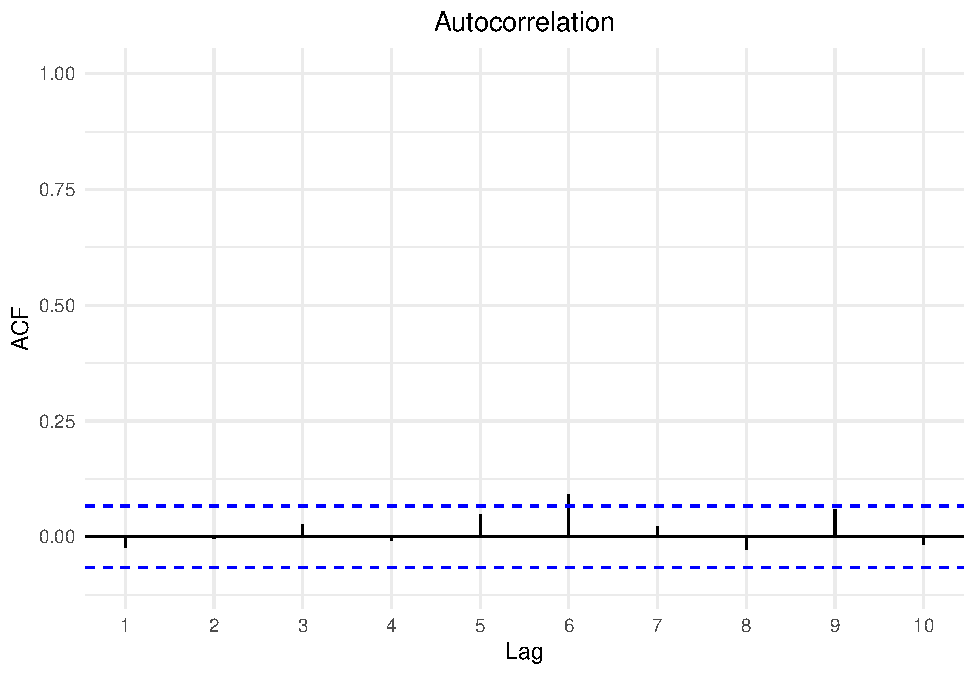
\includegraphics{SCMU_egg_model_files/figure-latex/acf-1.pdf} The first
value with 0 lag will always be autocorrelated because it's stacked on
itself. But after that, we want to see the values within the blue dotted
lines. There does not appear to be autocorrelation in the residuals.

\hypertarget{identifying-outliers}{%
\section{Identifying Outliers}\label{identifying-outliers}}

\url{https://qerm514.github.io/website/labs/week_03/diagnostics_and_errors.html\#unusual_observations}
\url{https://qerm514.github.io/website/homework/week_03/hw_03_diagnostics_key.pdf}
Calculate the studentized residuals to look for outliers

\begin{Shaded}
\begin{Highlighting}[]
\DocumentationTok{\#\# get studentized residuals}
\NormalTok{(stud\_e }\OtherTok{\textless{}{-}} \FunctionTok{rstudent}\NormalTok{(global\_mod))}
\end{Highlighting}
\end{Shaded}

\begin{verbatim}
##            1            2            3            4            5            6 
##  1.334692028 -1.432303962 -0.417831919  0.076619990 -1.126837630  0.216916981 
##            7            8            9           10           11           12 
## -0.826880478 -1.450616843 -0.203144114 -0.467319488  1.489091460  0.805841181 
##           13           14           15           16           17           18 
##  0.227967785 -1.138748660 -0.957882066  0.845018269 -1.216715706 -0.822294182 
##           19           20           21           22           23           24 
## -0.267352269  1.390594022 -1.216715706 -0.583806748 -1.077365634  1.381562004 
##           25           26           27           28           29           30 
##  0.133713679  0.214145892 -1.673382506 -0.708532092  0.712224053  1.372633482 
##           31           32           33           34           35           36 
##  0.056400801 -1.525830123  0.056400801 -1.076384817 -0.186666559  0.531278615 
##           37           38           39           40           41           42 
##  0.048685340 -1.461142191  0.245649304  0.461868921 -0.742033988  0.874635633 
##           43           44           45           46           47           48 
## -0.900261227  0.970947865 -1.622487352  0.475627812 -0.267352269 -0.019692242 
##           49           50           51           52           53           54 
##  0.260957027 -0.563804529 -0.598130938 -0.259450616  0.086953468  0.506459533 
##           55           56           57           58           59           60 
## -0.482167262  1.393179553 -1.182784114  0.498141330 -2.136341951 -1.468502916 
##           61           62           63           64           65           66 
##  0.974369907  1.288339556  0.152710509 -0.997215541 -1.138748660 -2.957215340 
##           67           68           69           70           71           72 
## -0.247204090 -2.431092485  0.870721913  1.140919160  0.902205474 -0.216310733 
##           73           74           75           76           77           78 
## -0.435312431 -0.308078585  0.790189055 -1.493543440 -2.773955087  0.904905192 
##           79           80           81           82           83           84 
## -2.008493985 -0.468816730  0.351797798 -1.428092365 -0.759021397  0.725122357 
##           85           86           87           88           89           90 
## -0.821010018 -1.896404891  1.461956800  0.973425978  0.434759960 -0.275249650 
##           91           92           93           94           95           96 
## -0.620142977  0.382019338  1.108469710  0.084835095  0.757298346 -0.208697740 
##           97           98           99          100          101          102 
##  0.379606443  0.127803063  0.957647605  0.436294735  0.393623959  0.196942913 
##          103          104          105          106          107          108 
## -1.057142678 -1.950051458 -0.245369619 -2.206043836 -0.722974893 -1.371681203 
##          109          110          111          112          113          114 
##  0.325043321 -0.164160591 -0.775055325  0.216410317 -0.038489038  0.524860316 
##          115          116          117          118          119          120 
## -0.450357972  0.129414760  1.589527955  0.973662110 -1.200511770 -1.231340008 
##          121          122          123          124          125          126 
##  1.471268881 -0.360534027 -1.920754837  0.874032701 -0.992297001  1.052309305 
##          127          128          129          130          131          132 
## -0.792496355 -0.233827956 -0.961959926  0.714295624 -0.356344443 -0.191620972 
##          133          134          135          136          137          138 
##  1.588709789 -0.578417428  0.759537822  1.524609141  0.612482243 -0.677440977 
##          139          140          141          142          143          144 
## -0.081153118  0.553672027  2.088498840  1.008845307  1.434094862 -1.585426134 
##          145          146          147          148          149          150 
##  0.220123333  0.543951564  0.186424001  0.483670760  0.068859292  0.712811644 
##          151          152          153          154          155          156 
##  0.866426016 -0.022065661 -1.250882909  1.097201240 -0.448696911  1.377438964 
##          157          158          159          160          161          162 
## -0.191956057 -0.584394548 -2.219988421  0.388703524 -0.584394548  0.639995429 
##          163          164          165          166          167          168 
## -1.429888543 -0.617355406  0.202494199  0.766049993 -1.287583193  0.784033132 
##          169          170          171          172          173          174 
##  2.097926225 -2.228252612  1.924884388  0.179418896 -2.783974589 -0.307287428 
##          175          176          177          178          179          180 
##  1.332289773  1.492884429  0.748692478 -0.867415899  0.018688978 -0.209494506 
##          181          182          183          184          185          186 
##  1.919784087 -2.322523709  1.283363429  0.577983977  0.309588486 -1.060247012 
##          187          188          189          190          191          192 
##  0.477076081  0.771646431  0.480120579  1.042083079 -0.318155687  1.129659592 
##          193          194          195          196          197          198 
##  0.528938013  0.487467725  0.319585433 -0.842365750 -0.555558992  0.561951510 
##          199          200          201          202          203          204 
##  1.764146945  1.054168325  0.375417742 -0.059894672 -1.492542275 -0.185182744 
##          205          206          207          208          209          210 
##  1.970780078  0.025533881  1.008612129  1.168977287 -0.763946396 -0.223150262 
##          211          212          213          214          215          216 
## -0.032383691 -2.248839586  0.368804746  1.473175112  0.998332220  0.270726910 
##          217          218          219          220          221          222 
##  1.320450433 -1.007768380  0.310401500 -1.299725605 -0.618838111 -0.906103777 
##          223          224          225          226          227          228 
##  1.622311938 -1.349318843 -2.629283562  0.699065538  0.379005478 -0.168999794 
##          229          230          231          232          233          234 
## -0.219144068  1.269938803  1.878282514  0.980690589 -0.032383691  1.262799170 
##          235          236          237          238          239          240 
##  0.731049982 -2.478824898  0.521448276  0.432731485  0.704826204  0.310042679 
##          241          242          243          244          245          246 
## -3.531928835 -1.653605688 -0.732534664  0.565541383  1.228494252 -0.683391873 
##          247          248          249          250          251          252 
##  0.188898068  0.071435567  0.071435567  1.600992158  1.708487560 -0.844312670 
##          253          254          255          256          257          258 
## -1.583085378 -0.576486323  1.292603577  0.147215416 -0.908309271 -0.674119864 
##          259          260          261          262          263          264 
## -1.539426252 -1.209221474  0.463038464 -0.427327667 -0.409499920 -0.141681823 
##          265          266          267          268          269          270 
##  0.524761239 -0.542135482  0.039750999 -0.525152710 -0.860733616  0.883203391 
##          271          272          273          274          275          276 
##  0.081139411  0.426668462 -0.973633484 -0.621307742  0.243157818 -0.905850273 
##          277          278          279          280          281          282 
##  0.328575685  0.936374330 -0.172909860 -0.313436030 -0.120304446  0.416748968 
##          283          284          285          286          287          288 
##  0.131563507 -0.142600294 -0.365001715  1.203179772 -0.284082902 -0.102167523 
##          289          290          291          292          293          294 
## -0.176324254  0.285503306  2.166220788 -0.497547716  0.550558552  0.863179727 
##          295          296          297          298          299          300 
##  0.222359952  0.684095734 -0.669172823  0.665097660 -0.746912331 -1.030868927 
##          301          302          303          304          305          306 
## -0.353537059  1.508550861  0.785540750  0.677680812  1.709687632  0.606925846 
##          307          308          309          310          311          312 
## -1.108031312  1.125220112 -0.072385519 -0.740125254  0.313247326  0.179798732 
##          313          314          315          316          317          318 
## -1.035271355  2.174832285  0.427251864 -0.388939916 -0.807445714  0.319277659 
##          319          320          321          322          323          324 
##  1.640882760  1.824439024  1.640882760  0.576017238  1.034645844  1.020429611 
##          325          326          327          328          329          330 
##  0.599904258  1.313601941  1.056157025 -0.333817851 -0.332900678  0.259317585 
##          331          332          333          334          335          336 
##  0.552119371 -0.857431613 -0.115897672 -0.878618297 -0.452555595 -0.091814872 
##          337          338          339          340          341          342 
##  0.589186177 -0.135024094  0.468325345 -0.022878337  0.881326939 -1.088938400 
##          343          344          345          346          347          348 
##  2.079446348  0.459628052  0.210035235  0.319277659  0.819480670 -0.623604980 
##          349          350          351          352          353          354 
## -0.689593457 -0.461992703 -1.080442099 -0.110565683 -0.490343260  0.059661674 
##          355          356          357          358          359          360 
##  0.037636999 -0.352366111 -1.436415778 -1.034452258  0.267560435 -0.251294926 
##          361          362          363          364          365          366 
##  0.012087687 -1.752631038 -0.100562438  0.065167725  0.131459790 -2.144567779 
##          367          368          369          370          371          372 
## -0.579338464  0.822658886 -0.561245098 -0.759414158  0.783210849  0.737264134 
##          373          374          375          376          377          378 
## -0.596095624  0.045280105 -0.630714814  0.047029479 -0.160409441 -0.503608986 
##          379          380          381          382          383          384 
##  0.920398795  0.354061758 -0.172444299  1.920587709  0.414445712  0.416217239 
##          385          386          387          388          389          390 
##  0.310178454 -1.337472815  1.149652173 -0.094094416  0.682050584  0.778700519 
##          391          392          393          394          395          396 
## -2.037402438  0.417928820 -0.651062247 -0.165157216  1.069483293  1.054022679 
##          397          398          399          400          401          402 
##  1.070311541  1.048869140  0.762755743 -0.327125560  1.589885223 -2.023032326 
##          403          404          405          406          407          408 
##  0.777070846  1.111753703 -1.010513104  1.458379679  0.812758115  0.764688320 
##          409          410          411          412          413          414 
## -0.233809707 -0.796833756 -0.539340901  0.370718729 -0.128184132  0.495230698 
##          415          416          417          418          419          420 
## -1.226647557 -0.316481314  0.209302551  0.264043920 -1.515356358  0.019742813 
##          421          422          423          424          425          426 
##  0.919533281 -1.624344748  0.412648633  0.810953458  0.191173140 -0.776403658 
##          427          428          429          430          431          432 
##  0.545601052 -0.100562438  0.503899407  0.053918055  1.221081077 -0.280743716 
##          433          434          435          436          437          438 
##  0.389216250 -0.424306566  0.322594290 -0.853302666  0.349644439  0.268371319 
##          439          440          441          442          443          444 
##  0.138891446 -0.722096326  1.105936102 -1.880365718  0.120598877 -0.147005096 
##          445          446          447          448          449          450 
## -0.294112394  1.246460135 -0.232380362 -1.163175978  0.211015784 -0.129844332 
##          451          452          453          454          455          456 
## -1.444540992 -0.328928391  0.195580589 -0.924757336 -0.298529413 -0.911894674 
##          457          458          459          460          461          462 
## -0.861458391 -0.477888209 -0.915723238  0.025209823 -0.312127085 -0.570574317 
##          463          464          465          466          467          468 
##  0.798247124  0.631270332  0.191237612 -0.926567081 -0.526171988 -0.591614371 
##          469          470          471          472          473          474 
##  0.270000280 -0.395183136 -0.521418900  1.303560865  0.984032761  1.361759335 
##          475          476          477          478          479          480 
##  0.727945943 -1.102917364 -0.350464984  1.126377991  0.976711722 -1.261391596 
##          481          482          483          484          485          486 
##  0.828699224  0.122539040 -0.438502640 -0.815444928  1.325261184 -0.652042464 
##          487          488          489          490          491          492 
## -0.054548086  0.250724984  0.034215726  1.180722307  0.398311516  0.663434271 
##          493          494          495          496          497          498 
##  1.367920422  0.262190807  1.601837131  0.804535794 -0.325357252 -0.279419171 
##          499          500          501          502          503          504 
##  0.644120014  0.241334918  0.477272903 -0.115879602  0.599100694 -0.152482955 
##          505          506          507          508          509          510 
##  0.712992352 -0.432096857 -0.500440837 -0.801587203 -0.279419171  1.301677709 
##          511          512          513          514          515          516 
##  0.392379329  0.029284735  0.113443300  0.618334574 -1.032720500  1.285897893 
##          517          518          519          520          521          522 
## -0.737004730  0.008529960 -0.184106347 -1.428840326  0.950470928  0.489982802 
##          523          524          525          526          527          528 
## -0.168750613  0.565563999 -0.866098875  0.235194397  0.543508727  1.384917371 
##          529          530          531          532          533          534 
## -1.022323722  0.611880071  0.675725414 -3.539073821  0.530900776  0.606484091 
##          535          536          537          538          539          540 
##  0.045769914  0.194089974 -6.483703648 -0.087662229 -0.694788801 -1.585320450 
##          541          542          543          544          545          546 
## -0.709704500  0.603173024 -0.801571288 -0.260162370 -0.725128940 -1.535642411 
##          547          548          549          550          551          552 
##  0.650374956  0.793532189  0.328340053 -0.239683398  1.112543369 -0.625394850 
##          553          554          555          556          557          558 
## -0.677953758  0.659491776 -0.512252679 -0.194499503  0.656160014 -1.388804235 
##          559          560          561          562          563          564 
## -1.096712603  0.326595353 -1.610838280 -0.252714049 -0.350352169  0.401425456 
##          565          566          567          568          569          570 
## -1.637888713  1.077826474 -0.537094251 -0.351723040  0.098406948  0.163603635 
##          571          572          573          574          575          576 
## -1.066134438  0.014844998  0.675994499 -0.743824056 -0.154525338 -0.681106680 
##          577          578          579          580          581          582 
## -0.034741215 -0.659600727  0.454428203 -0.336220336 -1.425115602  1.239797926 
##          583          584          585          586          587          588 
##  0.270099722 -0.731152024 -0.020049004  1.717304965  1.229523555  2.090600841 
##          589          590          591          592          593          594 
## -1.028680164  0.223822379 -0.228488049  1.092563061  1.162919645 -0.706150530 
##          595          596          597          598          599          600 
##  0.759265940 -0.193691499  0.473149512 -0.422253224 -0.641558018 -0.733302359 
##          601          602          603          604          605          606 
##  0.618067001  0.746637650  0.710153890 -0.427298732  0.129627897 -0.648691989 
##          607          608          609          610          611          612 
##  0.204925479  0.809877274  0.211536974  0.328982837  1.002712545  0.444592174 
##          613          614          615          616          617          618 
## -0.878808746 -0.137915845 -0.370540503  0.077824024  1.829253691 -0.825236825 
##          619          620          621          622          623          624 
## -0.905714862 -1.205511609  0.952529441 -1.003720043  0.151603205 -0.657948955 
##          625          626          627          628          629          630 
##  0.670076307  0.679932497  0.223052762  1.794093943  0.317646172 -0.037561735 
##          631          632          633          634          635          636 
##  0.603632662  0.075601032  0.744606568 -0.753781827  1.376174650  1.018472737 
##          637          638          639          640          641          642 
## -0.627598919  0.285069019  1.681989123  1.164767768 -0.496945402  1.264056613 
##          643          644          645          646          647          648 
## -0.645871064  1.190862364  0.948209881  1.598028663 -0.289341532  1.943238083 
##          649          650          651          652          653          654 
## -0.628599301 -1.080872128  1.661721948 -0.616969776 -0.171484945 -0.450649303 
##          655          656          657          658          659          660 
## -1.685028860  1.050100730 -1.331792914 -1.496377981  0.580046380  0.546044375 
##          661          662          663          664          665          666 
## -0.169016874  0.356653889 -1.266696515 -0.741331322 -0.043479587  0.688910145 
##          667          668          669          670          671          672 
##  0.368305435  0.190450336  0.342111202 -1.518064091  0.375706649  0.175882771 
##          673          674          675          676          677          678 
## -0.258464938  0.407369207 -0.042625697  0.596608218  1.162208276  1.562332633 
##          679          680          681          682          683          684 
##  0.613087131 -1.061229615  0.705764688 -0.261851827  1.087248374 -0.575825242 
##          685          686          687          688          689          690 
## -0.761225209  0.317741808 -0.645042683  0.004873608 -0.430732612 -0.549760568 
##          691          692          693          694          695          696 
## -1.185791315 -1.119520844  1.048421199 -0.143749041 -1.051777697 -0.932492769 
##          697          698          699          700          701          702 
## -3.320518439  1.392883927 -0.037754587  1.202943521 -2.178443845  0.692587177 
##          703          704          705          706          707          708 
## -1.374866270 -0.563712616 -0.532787375 -0.204833693 -0.581718391  0.354982088 
##          709          710          711          712          713          714 
##  0.973608783 -1.653135423  0.038822209  0.025005701 -2.211480498 -0.420387147 
##          715          716          717          718          719          720 
## -0.202998063  1.105977053  0.422080351 -0.496383556 -0.567930030 -0.805269491 
##          721          722          723          724          725          726 
##  0.572637822 -1.211386898 -0.275157155  0.672118818  0.291510377 -0.085337378 
##          727          728          729          730          731          732 
##  0.524818845  1.202236851  0.827854913  1.006412640 -0.715091473  0.506798497 
##          733          734          735          736          737          738 
##  1.681488706  0.013077719 -1.708287059  1.722620390 -0.625449432  0.457209997 
##          739          740          741          742          743          744 
##  1.213358500 -3.173489960 -0.067386333 -2.968176046  2.334709316  0.998735725 
##          745          746          747          748          749          750 
## -0.226577683  0.099573803  0.303680786  0.871487192  0.791472429 -1.191860476 
##          751          752          753          754          755          756 
## -0.218013354 -0.418396308 -0.902263924  0.358006859 -0.320681238  1.448666666 
##          757          758          759          760          761          762 
##  0.657205847  0.913131024  0.156680027 -2.402716419 -1.006579834 -0.543621651 
##          763          764          765          766          767          768 
## -0.428534785  0.563532474 -0.457906664 -0.696053247  0.018458497  0.472316891 
##          769          770          771          772          773          774 
##  2.302618349  0.711623679 -1.049792006  1.405722546  0.719037420  0.628666445 
##          775          776          777          778          779          780 
## -1.064783169  1.020647110 -0.539815463  1.570582173  0.871235849  1.060353044 
##          781          782          783          784          785          786 
##  0.491630659 -2.360920974  0.067567271 -0.018620710 -0.280920080  0.412712878 
##          787          788          789          790          791          792 
## -0.209777394 -0.004403171  1.619241133 -0.298997587 -0.516884736 -1.143123762 
##          793          794          795          796          797          798 
##  0.312197068  0.458310284  0.213865826 -0.776958440  0.801415821  0.268957771 
##          799          800          801          802          803          804 
##  0.423995816  0.757956837  0.969278916 -1.001084437 -0.757859889  0.942571409 
##          805          806          807          808          809          810 
## -0.420848873  0.542797779 -0.544159727 -0.306812869 -0.302136580 -0.172672305 
##          811          812          813          814          815          816 
## -0.616484276  0.242339785  1.990859498  0.494657073 -0.361841915  0.577207509 
##          817          818          819          820          821          822 
## -0.518749435  0.443198444 -0.063901024  0.928432367  0.624161309 -0.457352831 
##          823          824          825          826          827          828 
##  1.205283640  0.108774299 -0.307946541  1.524957889  0.103339030 -0.848204405 
##          829          830          831          832          833          834 
##  1.532303051  0.587828398 -2.004063992 -1.070193659 -6.671648537 -1.429125982 
##          835          836          837          838          839          840 
## -0.469176808  1.055296759  0.033576640 -0.277926679 -0.006865249 -0.802801123 
##          841          842          843          844          845          846 
## -0.499400841  0.963297348 -0.474700782 -0.069076969 -0.286323129  0.140656156 
##          847          848          849          850          851          852 
##  1.269751669 -1.272346739  0.572785243  0.454987895 -0.536771984  0.222953353 
##          853          854          855          856          857          858 
##  1.160220188 -0.597871149  0.136907466 -0.665052470  1.393024587  0.390066905 
##          859          860          861          862          863          864 
##  0.574223459 -0.914802854  0.608953652  1.076139169  1.522288597  0.936751371 
##          865          866          867          868          869          870 
## -0.408318552  1.383929139 -1.182638805  0.330590954  0.496854396  0.005407740 
##          871          872          873          874 
## -0.413636938  0.751023077 -0.010734196 -1.517560932
\end{verbatim}

\begin{Shaded}
\begin{Highlighting}[]
\DocumentationTok{\#\# get sample size}
\NormalTok{n }\OtherTok{\textless{}{-}} \FunctionTok{nrow}\NormalTok{(SCMUdf)}

\DocumentationTok{\#\# Bonferroni correction: alpha/n}
\NormalTok{alpha }\OtherTok{\textless{}{-}} \FloatTok{0.05}\SpecialCharTok{/}\NormalTok{n}

\DocumentationTok{\#\# critical t value}
\NormalTok{degf }\OtherTok{\textless{}{-}}\NormalTok{ n }\SpecialCharTok{{-}} \FunctionTok{length}\NormalTok{(}\FunctionTok{coef}\NormalTok{(global\_mod))}\SpecialCharTok{{-}}\DecValTok{1} \CommentTok{\# should be more due to REs?}
\NormalTok{t\_crit }\OtherTok{\textless{}{-}} \FunctionTok{qt}\NormalTok{(}\DecValTok{1} \SpecialCharTok{{-}}\NormalTok{ alpha}\SpecialCharTok{/}\DecValTok{2}\NormalTok{, degf)}

\DocumentationTok{\#\# compare t\_stud to t\_crit}
\FunctionTok{sum}\NormalTok{(stud\_e }\SpecialCharTok{\textgreater{}}\NormalTok{ t\_crit, }\AttributeTok{na.rm =} \ConstantTok{TRUE}\NormalTok{)}
\end{Highlighting}
\end{Shaded}

\begin{verbatim}
## [1] 0
\end{verbatim}

\hypertarget{cooks-distance}{%
\subsection{Cook's Distance}\label{cooks-distance}}

\begin{Shaded}
\begin{Highlighting}[]
\DocumentationTok{\#\# Cook\textquotesingle{}s D}
\NormalTok{cook }\OtherTok{\textless{}{-}} \FunctionTok{cooks.distance}\NormalTok{(global\_mod)}

\CommentTok{\# Plot the Cook\textquotesingle{}s Distance using the traditional 4/n criterion}
\NormalTok{sample\_size }\OtherTok{\textless{}{-}} \FunctionTok{nrow}\NormalTok{(SCMUdf)}
\FunctionTok{plot}\NormalTok{(cook, }\AttributeTok{pch=}\StringTok{"*"}\NormalTok{, }\AttributeTok{cex=}\DecValTok{2}\NormalTok{, }\AttributeTok{main=}\StringTok{"Influential Obs by Cooks distance"}\NormalTok{)  }\CommentTok{\# plot cook\textquotesingle{}s distance}
\FunctionTok{abline}\NormalTok{(}\AttributeTok{h =} \DecValTok{4}\SpecialCharTok{/}\NormalTok{sample\_size, }\AttributeTok{col=}\StringTok{"red"}\NormalTok{)  }\CommentTok{\# add cutoff line}
\FunctionTok{text}\NormalTok{(}\AttributeTok{x=}\DecValTok{1}\SpecialCharTok{:}\FunctionTok{length}\NormalTok{(cook)}\SpecialCharTok{+}\DecValTok{1}\NormalTok{, }\AttributeTok{y=}\NormalTok{cook, }\AttributeTok{labels=}\FunctionTok{ifelse}\NormalTok{(cook}\SpecialCharTok{\textgreater{}}\DecValTok{4}\SpecialCharTok{/}\NormalTok{sample\_size, }\FunctionTok{names}\NormalTok{(cook),}\StringTok{""}\NormalTok{), }\AttributeTok{col=}\StringTok{"red"}\NormalTok{)  }\CommentTok{\# add labels}
\end{Highlighting}
\end{Shaded}

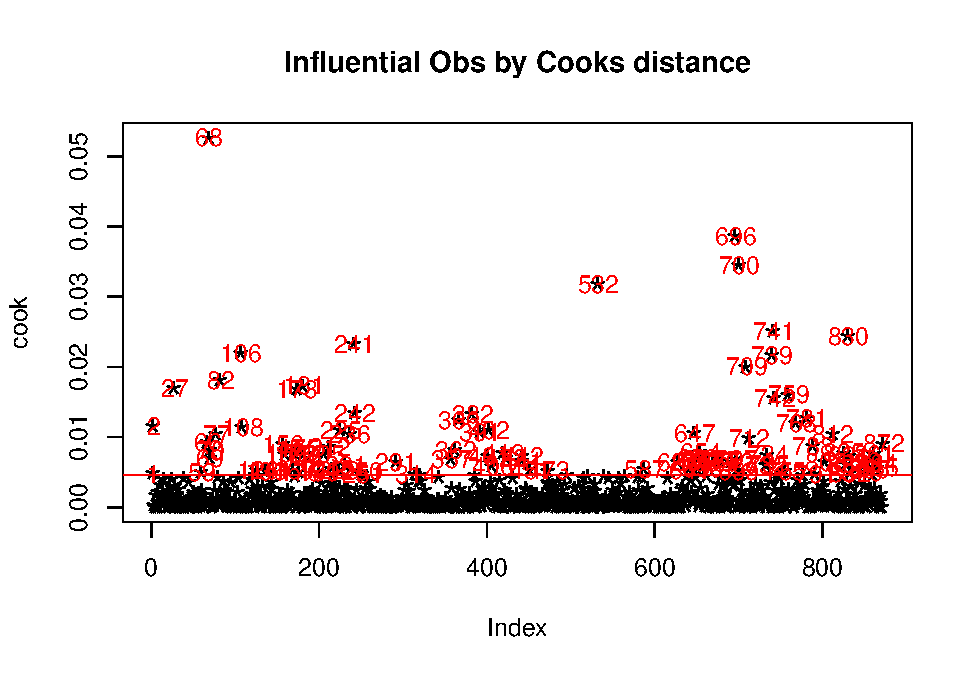
\includegraphics{SCMU_egg_model_files/figure-latex/cook-1.pdf}

\hypertarget{fit-candidate-models}{%
\section{Fit Candidate Models}\label{fit-candidate-models}}

\begin{Shaded}
\begin{Highlighting}[]
\DocumentationTok{\#\# create empty matrix for storing results}
\NormalTok{mod\_res }\OtherTok{\textless{}{-}} \FunctionTok{matrix}\NormalTok{(}\ConstantTok{NA}\NormalTok{, n\_mods, }\DecValTok{1}\NormalTok{)}
\FunctionTok{colnames}\NormalTok{(mod\_res) }\OtherTok{\textless{}{-}} \FunctionTok{c}\NormalTok{(}\StringTok{"AIC"}\NormalTok{)}

\DocumentationTok{\#\# fit models and store AIC \& BIC}
\ControlFlowTok{for}\NormalTok{(i }\ControlFlowTok{in} \DecValTok{1}\SpecialCharTok{:}\NormalTok{n\_mods) \{}
  \ControlFlowTok{if}\NormalTok{(i }\SpecialCharTok{==} \DecValTok{1}\NormalTok{) \{}
\NormalTok{    fmla }\OtherTok{\textless{}{-}} \StringTok{"Size \textasciitilde{} 1 + (1 | Plot)"}
\NormalTok{  \} }\ControlFlowTok{else}\NormalTok{ \{}
\NormalTok{    fmla }\OtherTok{\textless{}{-}} \FunctionTok{paste}\NormalTok{(}\StringTok{"Size \textasciitilde{} (1 | Plot) +"}\NormalTok{, }\FunctionTok{paste}\NormalTok{(cov\_names[use\_set[i,]], }\AttributeTok{collapse =} \StringTok{" + "}\NormalTok{))}
\NormalTok{  \}}
\NormalTok{  mod\_fit }\OtherTok{\textless{}{-}} \FunctionTok{lmer}\NormalTok{(}\FunctionTok{as.formula}\NormalTok{(fmla), }\AttributeTok{data =}\NormalTok{ SCMUdf, }\AttributeTok{REML =} \ConstantTok{TRUE}\NormalTok{)}
\NormalTok{  mod\_res[i,}\StringTok{"AIC"}\NormalTok{] }\OtherTok{\textless{}{-}} \FunctionTok{AIC}\NormalTok{(mod\_fit)}
\NormalTok{\}}

\DocumentationTok{\#\# create empty matrix for storing results}
\NormalTok{delta\_res }\OtherTok{\textless{}{-}} \FunctionTok{matrix}\NormalTok{(}\ConstantTok{NA}\NormalTok{, n\_mods, }\DecValTok{1}\NormalTok{)}
\FunctionTok{colnames}\NormalTok{(delta\_res) }\OtherTok{\textless{}{-}} \FunctionTok{c}\NormalTok{(}\StringTok{"deltaAIC"}\NormalTok{)}

\DocumentationTok{\#\# convert IC to deltaIC}
\NormalTok{delta\_res[,}\StringTok{"deltaAIC"}\NormalTok{] }\OtherTok{\textless{}{-}}\NormalTok{ mod\_res[,}\StringTok{"AIC"}\NormalTok{] }\SpecialCharTok{{-}} \FunctionTok{min}\NormalTok{(mod\_res[,}\StringTok{"AIC"}\NormalTok{])}
\NormalTok{(delta\_res }\OtherTok{\textless{}{-}} \FunctionTok{round}\NormalTok{(delta\_res, }\DecValTok{2}\NormalTok{)) }\CommentTok{\# round results}
\end{Highlighting}
\end{Shaded}

\begin{verbatim}
##       deltaAIC
##  [1,]    46.71
##  [2,]    30.00
##  [3,]    33.15
##  [4,]    16.13
##  [5,]    35.29
##  [6,]    18.40
##  [7,]    27.49
##  [8,]    10.44
##  [9,]    24.40
## [10,]     7.37
## [11,]    17.14
## [12,]     0.00
## [13,]    31.96
## [14,]    14.62
## [15,]    18.42
## [16,]     1.09
## [17,]    26.12
## [18,]     9.04
## [19,]    36.41
## [20,]    19.58
## [21,]    28.84
## [22,]    11.83
## [23,]    25.65
## [24,]     8.64
## [25,]    21.66
## [26,]     4.61
## [27,]    26.89
## [28,]     9.60
## [29,]    22.92
## [30,]     5.84
\end{verbatim}

\begin{Shaded}
\begin{Highlighting}[]
\DocumentationTok{\#\# "best" models from our set}
\NormalTok{cov\_names[use\_set[}\DecValTok{12}\NormalTok{,]] }\CommentTok{\# Egg order, BEUTI, NPGO}
\end{Highlighting}
\end{Shaded}

\begin{verbatim}
## [1] "EggOrder" "BEUTI"    "NPGO"
\end{verbatim}

\begin{Shaded}
\begin{Highlighting}[]
\NormalTok{cov\_names[use\_set[}\DecValTok{16}\NormalTok{,]] }\CommentTok{\# Egg order, NPGO, ONI}
\end{Highlighting}
\end{Shaded}

\begin{verbatim}
## [1] "EggOrder" "NPGO"     "ONI"
\end{verbatim}

\begin{Shaded}
\begin{Highlighting}[]
\NormalTok{cov\_names[use\_set[}\DecValTok{26}\NormalTok{,]] }\CommentTok{\# Egg order, ANCHL, BEUTI, SST (\textgreater{}2 AIC)}
\end{Highlighting}
\end{Shaded}

\begin{verbatim}
## [1] "EggOrder" "ANCHL"    "BEUTI"    "SST"
\end{verbatim}

\begin{Shaded}
\begin{Highlighting}[]
\NormalTok{cov\_names[use\_set[}\DecValTok{30}\NormalTok{,]] }\CommentTok{\# Egg order, PDO, SST (\textgreater{}2 AIC)}
\end{Highlighting}
\end{Shaded}

\begin{verbatim}
## [1] "EggOrder" "PDO"      "SST"
\end{verbatim}

\begin{Shaded}
\begin{Highlighting}[]
\NormalTok{cov\_names[use\_set[}\DecValTok{10}\NormalTok{,]] }\CommentTok{\# Egg order, NPGO (\textgreater{}2 AIC)}
\end{Highlighting}
\end{Shaded}

\begin{verbatim}
## [1] "EggOrder" "NPGO"
\end{verbatim}

\begin{Shaded}
\begin{Highlighting}[]
\NormalTok{cov\_names[use\_set[}\DecValTok{24}\NormalTok{,]] }\CommentTok{\# Egg order, BEUTI, SST (\textgreater{}2 AIC)}
\end{Highlighting}
\end{Shaded}

\begin{verbatim}
## [1] "EggOrder" "BEUTI"    "SST"
\end{verbatim}

\begin{Shaded}
\begin{Highlighting}[]
\DocumentationTok{\#\# run top models}
\NormalTok{topmod1 }\OtherTok{\textless{}{-}} \FunctionTok{lmer}\NormalTok{(Size }\SpecialCharTok{\textasciitilde{}}\NormalTok{ EggOrder }\SpecialCharTok{+}\NormalTok{ BEUTI }\SpecialCharTok{+}\NormalTok{ NPGO }\SpecialCharTok{+}\NormalTok{ (}\DecValTok{1} \SpecialCharTok{|}\NormalTok{ Plot), }\AttributeTok{data =}\NormalTok{ SCMUdf, }\AttributeTok{REML =} \ConstantTok{TRUE}\NormalTok{)}
\NormalTok{topmod2 }\OtherTok{\textless{}{-}} \FunctionTok{lmer}\NormalTok{(Size }\SpecialCharTok{\textasciitilde{}}\NormalTok{ EggOrder }\SpecialCharTok{+}\NormalTok{ NPGO }\SpecialCharTok{+}\NormalTok{ ONI }\SpecialCharTok{+}\NormalTok{ (}\DecValTok{1} \SpecialCharTok{|}\NormalTok{ Plot), }\AttributeTok{data =}\NormalTok{ SCMUdf, }\AttributeTok{REML =} \ConstantTok{TRUE}\NormalTok{)}
\NormalTok{topmod3 }\OtherTok{\textless{}{-}} \FunctionTok{lmer}\NormalTok{(Size }\SpecialCharTok{\textasciitilde{}}\NormalTok{ EggOrder }\SpecialCharTok{+}\NormalTok{ ANCHL }\SpecialCharTok{+}\NormalTok{ BEUTI }\SpecialCharTok{+}\NormalTok{ SST }\SpecialCharTok{+}\NormalTok{ (}\DecValTok{1} \SpecialCharTok{|}\NormalTok{ Plot), }\AttributeTok{data =}\NormalTok{ SCMUdf, }\AttributeTok{REML =} \ConstantTok{TRUE}\NormalTok{)}
\NormalTok{topmod4 }\OtherTok{\textless{}{-}} \FunctionTok{lmer}\NormalTok{(Size }\SpecialCharTok{\textasciitilde{}}\NormalTok{ EggOrder }\SpecialCharTok{+}\NormalTok{ PDO }\SpecialCharTok{+}\NormalTok{ SST }\SpecialCharTok{+}\NormalTok{ (}\DecValTok{1} \SpecialCharTok{|}\NormalTok{ Plot), }\AttributeTok{data =}\NormalTok{ SCMUdf, }\AttributeTok{REML =} \ConstantTok{TRUE}\NormalTok{)}
\NormalTok{topmod5 }\OtherTok{\textless{}{-}} \FunctionTok{lmer}\NormalTok{(Size }\SpecialCharTok{\textasciitilde{}}\NormalTok{ EggOrder }\SpecialCharTok{+}\NormalTok{ NPGO }\SpecialCharTok{+}\NormalTok{ (}\DecValTok{1} \SpecialCharTok{|}\NormalTok{ Plot), }\AttributeTok{data =}\NormalTok{ SCMUdf, }\AttributeTok{REML =} \ConstantTok{TRUE}\NormalTok{)}
\NormalTok{topmod6 }\OtherTok{\textless{}{-}}\FunctionTok{lmer}\NormalTok{(Size }\SpecialCharTok{\textasciitilde{}}\NormalTok{ EggOrder }\SpecialCharTok{+}\NormalTok{ BEUTI }\SpecialCharTok{+}\NormalTok{ SST }\SpecialCharTok{+}\NormalTok{ (}\DecValTok{1} \SpecialCharTok{|}\NormalTok{ Plot), }\AttributeTok{data =}\NormalTok{ SCMUdf, }\AttributeTok{REML =} \ConstantTok{TRUE}\NormalTok{)}

\DocumentationTok{\#\# Model selection table}
\NormalTok{AIC.tab }\OtherTok{\textless{}{-}} \FunctionTok{matrix}\NormalTok{(}\ConstantTok{NA}\NormalTok{, }\AttributeTok{nrow =} \DecValTok{6}\NormalTok{, }\AttributeTok{ncol =} \DecValTok{3}\NormalTok{) }\CommentTok{\# 6 rows for 6 top models}
\NormalTok{AIC.tab[}\DecValTok{1}\NormalTok{,}\DecValTok{1}\NormalTok{] }\OtherTok{\textless{}{-}} \FunctionTok{AIC}\NormalTok{(topmod1) }\CommentTok{\# AIC for topmod1 in first row, first column}
\NormalTok{AIC.tab[}\DecValTok{2}\NormalTok{,}\DecValTok{1}\NormalTok{] }\OtherTok{\textless{}{-}} \FunctionTok{AIC}\NormalTok{(topmod2) }\CommentTok{\# AIC for topmod2 in second row, first column}
\NormalTok{AIC.tab[}\DecValTok{3}\NormalTok{,}\DecValTok{1}\NormalTok{] }\OtherTok{\textless{}{-}} \FunctionTok{AIC}\NormalTok{(topmod3) }\CommentTok{\# AIC for topmod3 in second row, first column}
\NormalTok{AIC.tab[}\DecValTok{4}\NormalTok{,}\DecValTok{1}\NormalTok{] }\OtherTok{\textless{}{-}} \FunctionTok{AIC}\NormalTok{(topmod4) }\CommentTok{\# AIC for topmod4 in second row, first column}
\NormalTok{AIC.tab[}\DecValTok{5}\NormalTok{,}\DecValTok{1}\NormalTok{] }\OtherTok{\textless{}{-}} \FunctionTok{AIC}\NormalTok{(topmod5) }\CommentTok{\# AIC for topmod5 in second row, first column}
\NormalTok{AIC.tab[}\DecValTok{6}\NormalTok{,}\DecValTok{1}\NormalTok{] }\OtherTok{\textless{}{-}} \FunctionTok{AIC}\NormalTok{(topmod6) }\CommentTok{\# AIC for topmod6 in second row, first column}
\NormalTok{AIC.tab[,}\DecValTok{2}\NormalTok{] }\OtherTok{\textless{}{-}}\NormalTok{ AIC.tab[,}\DecValTok{1}\NormalTok{] }\SpecialCharTok{{-}} \FunctionTok{min}\NormalTok{(AIC.tab[,}\DecValTok{1}\NormalTok{]) }\CommentTok{\# calculate delta AIC}
\NormalTok{AIC.tab[,}\DecValTok{3}\NormalTok{] }\OtherTok{\textless{}{-}} \FunctionTok{exp}\NormalTok{(}\SpecialCharTok{{-}}\FloatTok{0.5}\SpecialCharTok{*}\NormalTok{AIC.tab[,}\DecValTok{2}\NormalTok{])}\SpecialCharTok{/}\NormalTok{(}\FunctionTok{sum}\NormalTok{(}\FunctionTok{exp}\NormalTok{(}\SpecialCharTok{{-}}\FloatTok{0.5}\SpecialCharTok{*}\NormalTok{AIC.tab[,}\DecValTok{2}\NormalTok{]))) }\CommentTok{\# calculate model weights}
\FunctionTok{colnames}\NormalTok{(AIC.tab) }\OtherTok{\textless{}{-}} \FunctionTok{c}\NormalTok{(}\StringTok{"AIC"}\NormalTok{, }\StringTok{"deltaAIC"}\NormalTok{, }\StringTok{"model\_weights"}\NormalTok{)}
\FunctionTok{print}\NormalTok{(AIC.tab)}
\end{Highlighting}
\end{Shaded}

\begin{verbatim}
##           AIC deltaAIC model_weights
## [1,] 10672.18 0.000000   0.564433704
## [2,] 10673.27 1.090108   0.327264573
## [3,] 10676.79 4.610461   0.056294240
## [4,] 10678.02 5.844698   0.030370563
## [5,] 10679.55 7.374504   0.014133824
## [6,] 10680.82 8.641014   0.007503096
\end{verbatim}

\hypertarget{top-models}{%
\section{Top Models}\label{top-models}}

Here we look at the top competitive models.

\hypertarget{top-model-1}{%
\subsection{Top Model 1}\label{top-model-1}}

\begin{Shaded}
\begin{Highlighting}[]
\NormalTok{topmod1 }\OtherTok{\textless{}{-}} \FunctionTok{lmer}\NormalTok{(Size }\SpecialCharTok{\textasciitilde{}}\NormalTok{ EggOrder }\SpecialCharTok{+}\NormalTok{ BEUTI }\SpecialCharTok{+}\NormalTok{ NPGO }\SpecialCharTok{+}\NormalTok{ (}\DecValTok{1} \SpecialCharTok{|}\NormalTok{ Plot), }\AttributeTok{data =}\NormalTok{ SCMUdf, }\AttributeTok{REML =} \ConstantTok{TRUE}\NormalTok{)}
\FunctionTok{summary}\NormalTok{(topmod1)  }
\end{Highlighting}
\end{Shaded}

\begin{verbatim}
## Linear mixed model fit by REML ['lmerMod']
## Formula: Size ~ EggOrder + BEUTI + NPGO + (1 | Plot)
##    Data: SCMUdf
## 
## REML criterion at convergence: 10660.2
## 
## Scaled residuals: 
##     Min      1Q  Median      3Q     Max 
## -6.6372 -0.6084  0.0419  0.6738  2.3199 
## 
## Random effects:
##  Groups   Name        Variance Std.Dev.
##  Plot     (Intercept)   239.4   15.47  
##  Residual             11850.7  108.86  
## Number of obs: 874, groups:  Plot, 8
## 
## Fixed effects:
##              Estimate Std. Error t value
## (Intercept)  1887.427      8.104 232.901
## EggOrderEgg2   32.931      9.148   3.600
## BEUTI         -10.404      4.954  -2.100
## NPGO          -15.062      3.711  -4.059
## 
## Correlation of Fixed Effects:
##             (Intr) EggOE2 BEUTI 
## EggOrdrEgg2 -0.236              
## BEUTI        0.078 -0.002       
## NPGO        -0.065  0.000 -0.230
\end{verbatim}

\hypertarget{top-model-2}{%
\subsection{Top Model 2}\label{top-model-2}}

\begin{Shaded}
\begin{Highlighting}[]
\NormalTok{topmod2 }\OtherTok{\textless{}{-}} \FunctionTok{lmer}\NormalTok{(Size }\SpecialCharTok{\textasciitilde{}}\NormalTok{ EggOrder }\SpecialCharTok{+}\NormalTok{ NPGO }\SpecialCharTok{+}\NormalTok{ ONI }\SpecialCharTok{+}\NormalTok{ (}\DecValTok{1} \SpecialCharTok{|}\NormalTok{ Plot), }\AttributeTok{data =}\NormalTok{ SCMUdf, }\AttributeTok{REML =} \ConstantTok{TRUE}\NormalTok{)}
\FunctionTok{summary}\NormalTok{(topmod2)}
\end{Highlighting}
\end{Shaded}

\begin{verbatim}
## Linear mixed model fit by REML ['lmerMod']
## Formula: Size ~ EggOrder + NPGO + ONI + (1 | Plot)
##    Data: SCMUdf
## 
## REML criterion at convergence: 10661.3
## 
## Scaled residuals: 
##     Min      1Q  Median      3Q     Max 
## -6.6268 -0.6169  0.0493  0.6724  2.3808 
## 
## Random effects:
##  Groups   Name        Variance Std.Dev.
##  Plot     (Intercept)   257.1   16.03  
##  Residual             11863.3  108.92  
## Number of obs: 874, groups:  Plot, 8
## 
## Fixed effects:
##              Estimate Std. Error t value
## (Intercept)  1887.453      8.301 227.380
## EggOrderEgg2   33.196      9.154   3.626
## NPGO          -13.532      4.052  -3.340
## ONI             9.174      5.103   1.798
## 
## Correlation of Fixed Effects:
##             (Intr) EggOE2 NPGO  
## EggOrdrEgg2 -0.232              
## NPGO        -0.079  0.009       
## ONI         -0.077  0.019  0.452
\end{verbatim}

\hypertarget{prediction}{%
\section{Prediction}\label{prediction}}

\begin{Shaded}
\begin{Highlighting}[]
\NormalTok{topmod1 }\OtherTok{\textless{}{-}} \FunctionTok{lmer}\NormalTok{(Size }\SpecialCharTok{\textasciitilde{}}\NormalTok{ EggOrder }\SpecialCharTok{+}\NormalTok{ BEUTI }\SpecialCharTok{+}\NormalTok{ NPGO }\SpecialCharTok{+}\NormalTok{ (}\DecValTok{1} \SpecialCharTok{|}\NormalTok{ Plot), }\AttributeTok{data =}\NormalTok{ SCMUdf, }\AttributeTok{REML =} \ConstantTok{TRUE}\NormalTok{)}
\NormalTok{topmod2 }\OtherTok{\textless{}{-}} \FunctionTok{lmer}\NormalTok{(Size }\SpecialCharTok{\textasciitilde{}}\NormalTok{ EggOrder }\SpecialCharTok{+}\NormalTok{ NPGO }\SpecialCharTok{+}\NormalTok{ ONI }\SpecialCharTok{+}\NormalTok{ (}\DecValTok{1} \SpecialCharTok{|}\NormalTok{ Plot), }\AttributeTok{data =}\NormalTok{ SCMUdf, }\AttributeTok{REML =} \ConstantTok{TRUE}\NormalTok{)}

\CommentTok{\# AIC tab for 2 top models}
\NormalTok{AIC.tab2 }\OtherTok{\textless{}{-}} \FunctionTok{matrix}\NormalTok{(}\ConstantTok{NA}\NormalTok{, }\AttributeTok{nrow =} \DecValTok{2}\NormalTok{, }\AttributeTok{ncol =} \DecValTok{3}\NormalTok{)}
\NormalTok{AIC.tab2[}\DecValTok{1}\NormalTok{,}\DecValTok{1}\NormalTok{] }\OtherTok{\textless{}{-}} \FunctionTok{AIC}\NormalTok{(topmod1)}
\NormalTok{AIC.tab2[}\DecValTok{2}\NormalTok{,}\DecValTok{1}\NormalTok{] }\OtherTok{\textless{}{-}} \FunctionTok{AIC}\NormalTok{(topmod2)}
\NormalTok{AIC.tab2[,}\DecValTok{2}\NormalTok{] }\OtherTok{\textless{}{-}}\NormalTok{ AIC.tab2[,}\DecValTok{1}\NormalTok{] }\SpecialCharTok{{-}} \FunctionTok{min}\NormalTok{(AIC.tab2[,}\DecValTok{1}\NormalTok{])}
\NormalTok{AIC.tab2[,}\DecValTok{3}\NormalTok{] }\OtherTok{\textless{}{-}} \FunctionTok{exp}\NormalTok{(}\SpecialCharTok{{-}}\FloatTok{0.5}\SpecialCharTok{*}\NormalTok{AIC.tab2[,}\DecValTok{2}\NormalTok{])}\SpecialCharTok{/}\NormalTok{(}\FunctionTok{sum}\NormalTok{(}\FunctionTok{exp}\NormalTok{(}\SpecialCharTok{{-}}\FloatTok{0.5}\SpecialCharTok{*}\NormalTok{AIC.tab2[,}\DecValTok{2}\NormalTok{])))}
\FunctionTok{print}\NormalTok{(AIC.tab2)}
\end{Highlighting}
\end{Shaded}

\begin{verbatim}
##          [,1]     [,2]      [,3]
## [1,] 10672.18 0.000000 0.6329873
## [2,] 10673.27 1.090108 0.3670127
\end{verbatim}

\begin{Shaded}
\begin{Highlighting}[]
\CommentTok{\#we want predictions with all predictors but one held constant, and then we\textquotesingle{}ll do this one{-}at{-}a{-}time for each of the predictors}
\CommentTok{\# this will allow us to produce nice plots looking at the marginal effect of each predictor }

\CommentTok{\#first, set up a dataset with everything at its mean value (except EggOrder)}
\FunctionTok{set.seed}\NormalTok{(}\DecValTok{1}\NormalTok{)}
\NormalTok{SCMU.null }\OtherTok{\textless{}{-}}\NormalTok{ SCMUdf[}\FunctionTok{c}\NormalTok{(}\DecValTok{1}\SpecialCharTok{:}\DecValTok{200}\NormalTok{),]}
\NormalTok{SCMU.null}\SpecialCharTok{$}\NormalTok{EggOrder }\OtherTok{\textless{}{-}} \FunctionTok{c}\NormalTok{(}\FunctionTok{rep}\NormalTok{(}\StringTok{"Egg1"}\NormalTok{,}\DecValTok{100}\NormalTok{),}\FunctionTok{rep}\NormalTok{(}\StringTok{"Egg2"}\NormalTok{,}\DecValTok{100}\NormalTok{))}
\NormalTok{SCMU.null}\SpecialCharTok{$}\NormalTok{BEUTI }\OtherTok{\textless{}{-}} \FunctionTok{mean}\NormalTok{(SCMUdf}\SpecialCharTok{$}\NormalTok{BEUTI) }
\NormalTok{SCMU.null}\SpecialCharTok{$}\NormalTok{NPGO }\OtherTok{\textless{}{-}} \FunctionTok{mean}\NormalTok{(SCMUdf}\SpecialCharTok{$}\NormalTok{NPGO) }
\NormalTok{SCMU.null}\SpecialCharTok{$}\NormalTok{ONI }\OtherTok{\textless{}{-}} \FunctionTok{mean}\NormalTok{(SCMUdf}\SpecialCharTok{$}\NormalTok{ONI) }
\NormalTok{SCMU.null}\SpecialCharTok{$}\NormalTok{ANCHL }\OtherTok{\textless{}{-}} \FunctionTok{mean}\NormalTok{(SCMUdf}\SpecialCharTok{$}\NormalTok{ANCHL) }
\NormalTok{SCMU.null}\SpecialCharTok{$}\NormalTok{PDO }\OtherTok{\textless{}{-}} \FunctionTok{mean}\NormalTok{(SCMUdf}\SpecialCharTok{$}\NormalTok{PDO)}
\NormalTok{SCMU.null}\SpecialCharTok{$}\NormalTok{SST }\OtherTok{\textless{}{-}} \FunctionTok{mean}\NormalTok{(SCMUdf}\SpecialCharTok{$}\NormalTok{SST)}
\CommentTok{\#I\textquotesingle{}m pretty sure you need some values of plot and observer but it doesn\textquotesingle{}t matter which ones because we\textquotesingle{}re not going to condition on these}

\NormalTok{SCMU.null}\SpecialCharTok{$}\NormalTok{Plot }\OtherTok{\textless{}{-}} \FunctionTok{sample}\NormalTok{(SCMUdf}\SpecialCharTok{$}\NormalTok{Plot,}\DecValTok{200}\NormalTok{,}\AttributeTok{replace =} \ConstantTok{TRUE}\NormalTok{)}
\CommentTok{\#SCMU.null$Observer \textless{}{-} sample(SCMUdf$Observer,200,replace = TRUE)}
\end{Highlighting}
\end{Shaded}

\hypertarget{beuti}{%
\subsection{BEUTI}\label{beuti}}

\begin{Shaded}
\begin{Highlighting}[]
\CommentTok{\#then vary just one predictor at a time for prediction. For example, create the dataset SCMU. BEUTI that will be used for predictions where the only thing that values is BEUTI }
\NormalTok{SCMU.BEUTI }\OtherTok{\textless{}{-}}\NormalTok{ SCMU.null}
\NormalTok{SCMU.BEUTI}\SpecialCharTok{$}\NormalTok{BEUTI }\OtherTok{\textless{}{-}} \FunctionTok{rep}\NormalTok{(}\FunctionTok{seq}\NormalTok{(}\AttributeTok{from =} \FunctionTok{min}\NormalTok{(SCMUdf}\SpecialCharTok{$}\NormalTok{BEUTI),}\AttributeTok{to =} \FunctionTok{max}\NormalTok{(SCMUdf}\SpecialCharTok{$}\NormalTok{BEUTI),}\AttributeTok{length.out =} \DecValTok{100}\NormalTok{),}\DecValTok{2}\NormalTok{)}

\CommentTok{\#PREDICT FOR SCMU.BEUTI}
\CommentTok{\#Pull together the random effects (do we want the models with)}

\CommentTok{\# obs.sd.1 \textless{}{-} as.data.frame(VarCorr(bm1))$sdcor[1]}
\CommentTok{\# plot.sd.1 \textless{}{-} as.data.frame(VarCorr(bm1))$sdcor[2]}
\CommentTok{\# resid.sd.1 \textless{}{-} as.data.frame(VarCorr(bm1))$sdcor[3]}
\CommentTok{\# }
\CommentTok{\# obs.sd.2 \textless{}{-} as.data.frame(VarCorr(bm2))$sdcor[1]}
\CommentTok{\# plot.sd.2 \textless{}{-} as.data.frame(VarCorr(bm2))$sdcor[2]}
\CommentTok{\# resid.sd.2 \textless{}{-} as.data.frame(VarCorr(bm2))$sdcor[3]}
\CommentTok{\# }
\CommentTok{\# obs.sd.3 \textless{}{-} as.data.frame(VarCorr(bm3))$sdcor[1]}
\CommentTok{\# plot.sd.3 \textless{}{-} as.data.frame(VarCorr(bm3))$sdcor[2]}
\CommentTok{\# resid.sd.3 \textless{}{-} as.data.frame(VarCorr(bm3))$sdcor[3]}

\NormalTok{plot.sd}\FloatTok{.1} \OtherTok{\textless{}{-}} \FunctionTok{as.data.frame}\NormalTok{(}\FunctionTok{VarCorr}\NormalTok{(topmod1))}\SpecialCharTok{$}\NormalTok{sdcor[}\DecValTok{1}\NormalTok{]}
\NormalTok{resid.sd}\FloatTok{.1} \OtherTok{\textless{}{-}} \FunctionTok{as.data.frame}\NormalTok{(}\FunctionTok{VarCorr}\NormalTok{(topmod1))}\SpecialCharTok{$}\NormalTok{sdcor[}\DecValTok{2}\NormalTok{]}

\NormalTok{plot.sd}\FloatTok{.2} \OtherTok{\textless{}{-}} \FunctionTok{as.data.frame}\NormalTok{(}\FunctionTok{VarCorr}\NormalTok{(topmod2))}\SpecialCharTok{$}\NormalTok{sdcor[}\DecValTok{1}\NormalTok{]}
\NormalTok{resid.sd}\FloatTok{.2} \OtherTok{\textless{}{-}} \FunctionTok{as.data.frame}\NormalTok{(}\FunctionTok{VarCorr}\NormalTok{(topmod2))}\SpecialCharTok{$}\NormalTok{sdcor[}\DecValTok{2}\NormalTok{]}

\NormalTok{sims }\OtherTok{\textless{}{-}} \DecValTok{10000}

\CommentTok{\# pv \textless{}{-} matrix(nrow = sims, ncol = nrow(SCMU.BEUTI))}
\CommentTok{\# for(i in 1:sims)\{}
\CommentTok{\#   \#choose a model }
\CommentTok{\#   model \textless{}{-} which(rmultinom(n = 1, size = 1,prob = c(AIC.tab[,3]))==1)}
\CommentTok{\#   if(model == 1)\{}
\CommentTok{\#     \#we simulate conditioning on no specific random effects levels}
\CommentTok{\#     y \textless{}{-} unlist(simulate(bm1))}
\CommentTok{\#     bmod \textless{}{-} refit(bm1,y)}
\CommentTok{\#     pv[i,] \textless{}{-} predict(bmod, re.form = \textasciitilde{}0, newdata = SCMU.BEUTI) + rnorm(1,0,sd=obs.sd.1) + rnorm(1,0,sd=plot.sd.1) + rnorm(1,0,sd=resid.sd.1)}
\CommentTok{\#   \}}
\CommentTok{\#   if(model == 2)\{}
\CommentTok{\#     \#we simulate conditioning on no specific random effects levels}
\CommentTok{\#     y \textless{}{-} unlist(simulate(bm2))}
\CommentTok{\#     bmod \textless{}{-} refit(bm2,y)}
\CommentTok{\#     pv[i,] \textless{}{-} predict(bmod, re.form = \textasciitilde{}0, newdata = SCMU.BEUTI) + rnorm(1,0,sd=obs.sd.2) + rnorm(1,0,sd=plot.sd.2) + rnorm(1,0,sd=resid.sd.2)}
\CommentTok{\#   \}}
\CommentTok{\#   if(model == 3)\{}
\CommentTok{\#     \#we simulate conditioning on no specific random effects levels}
\CommentTok{\#     y \textless{}{-} unlist(simulate(bm3))}
\CommentTok{\#     bmod \textless{}{-} refit(bm3,y)}
\CommentTok{\#     pv[i,] \textless{}{-} predict(bmod, re.form = \textasciitilde{}0, newdata = SCMU.BEUTI) + rnorm(1,0,sd=obs.sd.3) + rnorm(1,0,sd=plot.sd.3) + rnorm(1,0,sd=resid.sd.3)}
\CommentTok{\#   \}}
\CommentTok{\# \}  }

\DocumentationTok{\#\# Marcela tried updating}
\NormalTok{pv.BEUTI }\OtherTok{\textless{}{-}} \FunctionTok{matrix}\NormalTok{(}\AttributeTok{nrow =}\NormalTok{ sims, }\AttributeTok{ncol =} \FunctionTok{nrow}\NormalTok{(SCMU.BEUTI))}
\ControlFlowTok{for}\NormalTok{(i }\ControlFlowTok{in} \DecValTok{1}\SpecialCharTok{:}\NormalTok{sims)\{}
  \CommentTok{\#choose a model }
\NormalTok{  model }\OtherTok{\textless{}{-}} \FunctionTok{which}\NormalTok{(}\FunctionTok{rmultinom}\NormalTok{(}\AttributeTok{n =} \DecValTok{1}\NormalTok{, }\AttributeTok{size =} \DecValTok{1}\NormalTok{,}\AttributeTok{prob =} \FunctionTok{c}\NormalTok{(AIC.tab2[,}\DecValTok{3}\NormalTok{]))}\SpecialCharTok{==}\DecValTok{1}\NormalTok{)}
  \ControlFlowTok{if}\NormalTok{(model }\SpecialCharTok{==} \DecValTok{1}\NormalTok{)\{}
    \CommentTok{\#we simulate conditioning on no specific random effects levels}
\NormalTok{    y }\OtherTok{\textless{}{-}} \FunctionTok{unlist}\NormalTok{(}\FunctionTok{simulate}\NormalTok{(topmod1))}
\NormalTok{    bmod }\OtherTok{\textless{}{-}} \FunctionTok{refit}\NormalTok{(topmod1,y)}
\NormalTok{    pv.BEUTI[i,] }\OtherTok{\textless{}{-}} \FunctionTok{predict}\NormalTok{(bmod, }\AttributeTok{re.form =} \SpecialCharTok{\textasciitilde{}}\DecValTok{0}\NormalTok{, }\AttributeTok{newdata =}\NormalTok{ SCMU.BEUTI) }\SpecialCharTok{+} \FunctionTok{rnorm}\NormalTok{(}\DecValTok{1}\NormalTok{,}\DecValTok{0}\NormalTok{,}\AttributeTok{sd=}\NormalTok{plot.sd}\FloatTok{.1}\NormalTok{) }\SpecialCharTok{+} \FunctionTok{rnorm}\NormalTok{(}\DecValTok{1}\NormalTok{,}\DecValTok{0}\NormalTok{,}\AttributeTok{sd=}\NormalTok{resid.sd}\FloatTok{.1}\NormalTok{)}
\NormalTok{  \}}
  \ControlFlowTok{if}\NormalTok{(model }\SpecialCharTok{==} \DecValTok{2}\NormalTok{)\{}
    \CommentTok{\#we simulate conditioning on no specific random effects levels}
\NormalTok{    y }\OtherTok{\textless{}{-}} \FunctionTok{unlist}\NormalTok{(}\FunctionTok{simulate}\NormalTok{(topmod2))}
\NormalTok{    bmod }\OtherTok{\textless{}{-}} \FunctionTok{refit}\NormalTok{(topmod2,y)}
\NormalTok{    pv.BEUTI[i,] }\OtherTok{\textless{}{-}} \FunctionTok{predict}\NormalTok{(bmod, }\AttributeTok{re.form =} \SpecialCharTok{\textasciitilde{}}\DecValTok{0}\NormalTok{, }\AttributeTok{newdata =}\NormalTok{ SCMU.BEUTI) }\SpecialCharTok{+} \FunctionTok{rnorm}\NormalTok{(}\DecValTok{1}\NormalTok{,}\DecValTok{0}\NormalTok{,}\AttributeTok{sd=}\NormalTok{plot.sd}\FloatTok{.2}\NormalTok{) }\SpecialCharTok{+} \FunctionTok{rnorm}\NormalTok{(}\DecValTok{1}\NormalTok{,}\DecValTok{0}\NormalTok{,}\AttributeTok{sd=}\NormalTok{resid.sd}\FloatTok{.2}\NormalTok{)}
\NormalTok{  \}}
\NormalTok{\}  }
\end{Highlighting}
\end{Shaded}

\begin{verbatim}
## boundary (singular) fit: see ?isSingular
## boundary (singular) fit: see ?isSingular
## boundary (singular) fit: see ?isSingular
## boundary (singular) fit: see ?isSingular
## boundary (singular) fit: see ?isSingular
## boundary (singular) fit: see ?isSingular
## boundary (singular) fit: see ?isSingular
## boundary (singular) fit: see ?isSingular
## boundary (singular) fit: see ?isSingular
## boundary (singular) fit: see ?isSingular
## boundary (singular) fit: see ?isSingular
## boundary (singular) fit: see ?isSingular
## boundary (singular) fit: see ?isSingular
## boundary (singular) fit: see ?isSingular
## boundary (singular) fit: see ?isSingular
## boundary (singular) fit: see ?isSingular
## boundary (singular) fit: see ?isSingular
## boundary (singular) fit: see ?isSingular
## boundary (singular) fit: see ?isSingular
## boundary (singular) fit: see ?isSingular
## boundary (singular) fit: see ?isSingular
## boundary (singular) fit: see ?isSingular
## boundary (singular) fit: see ?isSingular
## boundary (singular) fit: see ?isSingular
## boundary (singular) fit: see ?isSingular
## boundary (singular) fit: see ?isSingular
## boundary (singular) fit: see ?isSingular
## boundary (singular) fit: see ?isSingular
## boundary (singular) fit: see ?isSingular
## boundary (singular) fit: see ?isSingular
## boundary (singular) fit: see ?isSingular
## boundary (singular) fit: see ?isSingular
## boundary (singular) fit: see ?isSingular
## boundary (singular) fit: see ?isSingular
## boundary (singular) fit: see ?isSingular
## boundary (singular) fit: see ?isSingular
## boundary (singular) fit: see ?isSingular
## boundary (singular) fit: see ?isSingular
## boundary (singular) fit: see ?isSingular
## boundary (singular) fit: see ?isSingular
## boundary (singular) fit: see ?isSingular
## boundary (singular) fit: see ?isSingular
## boundary (singular) fit: see ?isSingular
## boundary (singular) fit: see ?isSingular
## boundary (singular) fit: see ?isSingular
## boundary (singular) fit: see ?isSingular
## boundary (singular) fit: see ?isSingular
## boundary (singular) fit: see ?isSingular
## boundary (singular) fit: see ?isSingular
## boundary (singular) fit: see ?isSingular
## boundary (singular) fit: see ?isSingular
## boundary (singular) fit: see ?isSingular
## boundary (singular) fit: see ?isSingular
## boundary (singular) fit: see ?isSingular
## boundary (singular) fit: see ?isSingular
## boundary (singular) fit: see ?isSingular
## boundary (singular) fit: see ?isSingular
## boundary (singular) fit: see ?isSingular
## boundary (singular) fit: see ?isSingular
## boundary (singular) fit: see ?isSingular
## boundary (singular) fit: see ?isSingular
## boundary (singular) fit: see ?isSingular
## boundary (singular) fit: see ?isSingular
## boundary (singular) fit: see ?isSingular
## boundary (singular) fit: see ?isSingular
## boundary (singular) fit: see ?isSingular
## boundary (singular) fit: see ?isSingular
## boundary (singular) fit: see ?isSingular
## boundary (singular) fit: see ?isSingular
## boundary (singular) fit: see ?isSingular
## boundary (singular) fit: see ?isSingular
## boundary (singular) fit: see ?isSingular
## boundary (singular) fit: see ?isSingular
## boundary (singular) fit: see ?isSingular
## boundary (singular) fit: see ?isSingular
## boundary (singular) fit: see ?isSingular
## boundary (singular) fit: see ?isSingular
## boundary (singular) fit: see ?isSingular
## boundary (singular) fit: see ?isSingular
## boundary (singular) fit: see ?isSingular
## boundary (singular) fit: see ?isSingular
## boundary (singular) fit: see ?isSingular
## boundary (singular) fit: see ?isSingular
## boundary (singular) fit: see ?isSingular
## boundary (singular) fit: see ?isSingular
## boundary (singular) fit: see ?isSingular
## boundary (singular) fit: see ?isSingular
## boundary (singular) fit: see ?isSingular
## boundary (singular) fit: see ?isSingular
## boundary (singular) fit: see ?isSingular
## boundary (singular) fit: see ?isSingular
## boundary (singular) fit: see ?isSingular
## boundary (singular) fit: see ?isSingular
## boundary (singular) fit: see ?isSingular
## boundary (singular) fit: see ?isSingular
## boundary (singular) fit: see ?isSingular
## boundary (singular) fit: see ?isSingular
## boundary (singular) fit: see ?isSingular
## boundary (singular) fit: see ?isSingular
## boundary (singular) fit: see ?isSingular
## boundary (singular) fit: see ?isSingular
## boundary (singular) fit: see ?isSingular
## boundary (singular) fit: see ?isSingular
## boundary (singular) fit: see ?isSingular
## boundary (singular) fit: see ?isSingular
## boundary (singular) fit: see ?isSingular
## boundary (singular) fit: see ?isSingular
## boundary (singular) fit: see ?isSingular
## boundary (singular) fit: see ?isSingular
## boundary (singular) fit: see ?isSingular
## boundary (singular) fit: see ?isSingular
## boundary (singular) fit: see ?isSingular
## boundary (singular) fit: see ?isSingular
## boundary (singular) fit: see ?isSingular
## boundary (singular) fit: see ?isSingular
## boundary (singular) fit: see ?isSingular
## boundary (singular) fit: see ?isSingular
## boundary (singular) fit: see ?isSingular
## boundary (singular) fit: see ?isSingular
## boundary (singular) fit: see ?isSingular
## boundary (singular) fit: see ?isSingular
## boundary (singular) fit: see ?isSingular
## boundary (singular) fit: see ?isSingular
## boundary (singular) fit: see ?isSingular
## boundary (singular) fit: see ?isSingular
## boundary (singular) fit: see ?isSingular
## boundary (singular) fit: see ?isSingular
## boundary (singular) fit: see ?isSingular
## boundary (singular) fit: see ?isSingular
## boundary (singular) fit: see ?isSingular
## boundary (singular) fit: see ?isSingular
## boundary (singular) fit: see ?isSingular
## boundary (singular) fit: see ?isSingular
## boundary (singular) fit: see ?isSingular
## boundary (singular) fit: see ?isSingular
## boundary (singular) fit: see ?isSingular
## boundary (singular) fit: see ?isSingular
## boundary (singular) fit: see ?isSingular
## boundary (singular) fit: see ?isSingular
## boundary (singular) fit: see ?isSingular
## boundary (singular) fit: see ?isSingular
## boundary (singular) fit: see ?isSingular
## boundary (singular) fit: see ?isSingular
## boundary (singular) fit: see ?isSingular
## boundary (singular) fit: see ?isSingular
## boundary (singular) fit: see ?isSingular
## boundary (singular) fit: see ?isSingular
## boundary (singular) fit: see ?isSingular
## boundary (singular) fit: see ?isSingular
## boundary (singular) fit: see ?isSingular
## boundary (singular) fit: see ?isSingular
## boundary (singular) fit: see ?isSingular
## boundary (singular) fit: see ?isSingular
## boundary (singular) fit: see ?isSingular
## boundary (singular) fit: see ?isSingular
## boundary (singular) fit: see ?isSingular
## boundary (singular) fit: see ?isSingular
## boundary (singular) fit: see ?isSingular
## boundary (singular) fit: see ?isSingular
## boundary (singular) fit: see ?isSingular
## boundary (singular) fit: see ?isSingular
## boundary (singular) fit: see ?isSingular
## boundary (singular) fit: see ?isSingular
## boundary (singular) fit: see ?isSingular
## boundary (singular) fit: see ?isSingular
## boundary (singular) fit: see ?isSingular
## boundary (singular) fit: see ?isSingular
## boundary (singular) fit: see ?isSingular
## boundary (singular) fit: see ?isSingular
## boundary (singular) fit: see ?isSingular
## boundary (singular) fit: see ?isSingular
## boundary (singular) fit: see ?isSingular
## boundary (singular) fit: see ?isSingular
## boundary (singular) fit: see ?isSingular
## boundary (singular) fit: see ?isSingular
## boundary (singular) fit: see ?isSingular
## boundary (singular) fit: see ?isSingular
## boundary (singular) fit: see ?isSingular
## boundary (singular) fit: see ?isSingular
## boundary (singular) fit: see ?isSingular
## boundary (singular) fit: see ?isSingular
## boundary (singular) fit: see ?isSingular
## boundary (singular) fit: see ?isSingular
## boundary (singular) fit: see ?isSingular
## boundary (singular) fit: see ?isSingular
## boundary (singular) fit: see ?isSingular
## boundary (singular) fit: see ?isSingular
## boundary (singular) fit: see ?isSingular
## boundary (singular) fit: see ?isSingular
## boundary (singular) fit: see ?isSingular
## boundary (singular) fit: see ?isSingular
## boundary (singular) fit: see ?isSingular
## boundary (singular) fit: see ?isSingular
## boundary (singular) fit: see ?isSingular
## boundary (singular) fit: see ?isSingular
## boundary (singular) fit: see ?isSingular
## boundary (singular) fit: see ?isSingular
## boundary (singular) fit: see ?isSingular
## boundary (singular) fit: see ?isSingular
## boundary (singular) fit: see ?isSingular
## boundary (singular) fit: see ?isSingular
## boundary (singular) fit: see ?isSingular
## boundary (singular) fit: see ?isSingular
## boundary (singular) fit: see ?isSingular
## boundary (singular) fit: see ?isSingular
## boundary (singular) fit: see ?isSingular
## boundary (singular) fit: see ?isSingular
## boundary (singular) fit: see ?isSingular
## boundary (singular) fit: see ?isSingular
## boundary (singular) fit: see ?isSingular
## boundary (singular) fit: see ?isSingular
## boundary (singular) fit: see ?isSingular
## boundary (singular) fit: see ?isSingular
## boundary (singular) fit: see ?isSingular
## boundary (singular) fit: see ?isSingular
## boundary (singular) fit: see ?isSingular
## boundary (singular) fit: see ?isSingular
## boundary (singular) fit: see ?isSingular
## boundary (singular) fit: see ?isSingular
## boundary (singular) fit: see ?isSingular
## boundary (singular) fit: see ?isSingular
## boundary (singular) fit: see ?isSingular
## boundary (singular) fit: see ?isSingular
## boundary (singular) fit: see ?isSingular
## boundary (singular) fit: see ?isSingular
## boundary (singular) fit: see ?isSingular
## boundary (singular) fit: see ?isSingular
## boundary (singular) fit: see ?isSingular
## boundary (singular) fit: see ?isSingular
## boundary (singular) fit: see ?isSingular
## boundary (singular) fit: see ?isSingular
## boundary (singular) fit: see ?isSingular
## boundary (singular) fit: see ?isSingular
## boundary (singular) fit: see ?isSingular
## boundary (singular) fit: see ?isSingular
## boundary (singular) fit: see ?isSingular
## boundary (singular) fit: see ?isSingular
## boundary (singular) fit: see ?isSingular
## boundary (singular) fit: see ?isSingular
## boundary (singular) fit: see ?isSingular
## boundary (singular) fit: see ?isSingular
## boundary (singular) fit: see ?isSingular
## boundary (singular) fit: see ?isSingular
## boundary (singular) fit: see ?isSingular
## boundary (singular) fit: see ?isSingular
## boundary (singular) fit: see ?isSingular
## boundary (singular) fit: see ?isSingular
## boundary (singular) fit: see ?isSingular
## boundary (singular) fit: see ?isSingular
## boundary (singular) fit: see ?isSingular
## boundary (singular) fit: see ?isSingular
## boundary (singular) fit: see ?isSingular
## boundary (singular) fit: see ?isSingular
## boundary (singular) fit: see ?isSingular
## boundary (singular) fit: see ?isSingular
## boundary (singular) fit: see ?isSingular
## boundary (singular) fit: see ?isSingular
## boundary (singular) fit: see ?isSingular
## boundary (singular) fit: see ?isSingular
## boundary (singular) fit: see ?isSingular
## boundary (singular) fit: see ?isSingular
## boundary (singular) fit: see ?isSingular
## boundary (singular) fit: see ?isSingular
## boundary (singular) fit: see ?isSingular
## boundary (singular) fit: see ?isSingular
## boundary (singular) fit: see ?isSingular
## boundary (singular) fit: see ?isSingular
## boundary (singular) fit: see ?isSingular
## boundary (singular) fit: see ?isSingular
## boundary (singular) fit: see ?isSingular
## boundary (singular) fit: see ?isSingular
## boundary (singular) fit: see ?isSingular
## boundary (singular) fit: see ?isSingular
## boundary (singular) fit: see ?isSingular
## boundary (singular) fit: see ?isSingular
## boundary (singular) fit: see ?isSingular
## boundary (singular) fit: see ?isSingular
## boundary (singular) fit: see ?isSingular
## boundary (singular) fit: see ?isSingular
## boundary (singular) fit: see ?isSingular
## boundary (singular) fit: see ?isSingular
## boundary (singular) fit: see ?isSingular
## boundary (singular) fit: see ?isSingular
## boundary (singular) fit: see ?isSingular
## boundary (singular) fit: see ?isSingular
## boundary (singular) fit: see ?isSingular
## boundary (singular) fit: see ?isSingular
## boundary (singular) fit: see ?isSingular
## boundary (singular) fit: see ?isSingular
## boundary (singular) fit: see ?isSingular
## boundary (singular) fit: see ?isSingular
## boundary (singular) fit: see ?isSingular
## boundary (singular) fit: see ?isSingular
## boundary (singular) fit: see ?isSingular
## boundary (singular) fit: see ?isSingular
## boundary (singular) fit: see ?isSingular
## boundary (singular) fit: see ?isSingular
## boundary (singular) fit: see ?isSingular
## boundary (singular) fit: see ?isSingular
## boundary (singular) fit: see ?isSingular
## boundary (singular) fit: see ?isSingular
## boundary (singular) fit: see ?isSingular
## boundary (singular) fit: see ?isSingular
## boundary (singular) fit: see ?isSingular
## boundary (singular) fit: see ?isSingular
## boundary (singular) fit: see ?isSingular
## boundary (singular) fit: see ?isSingular
## boundary (singular) fit: see ?isSingular
## boundary (singular) fit: see ?isSingular
## boundary (singular) fit: see ?isSingular
## boundary (singular) fit: see ?isSingular
## boundary (singular) fit: see ?isSingular
## boundary (singular) fit: see ?isSingular
## boundary (singular) fit: see ?isSingular
## boundary (singular) fit: see ?isSingular
## boundary (singular) fit: see ?isSingular
## boundary (singular) fit: see ?isSingular
## boundary (singular) fit: see ?isSingular
## boundary (singular) fit: see ?isSingular
## boundary (singular) fit: see ?isSingular
## boundary (singular) fit: see ?isSingular
## boundary (singular) fit: see ?isSingular
## boundary (singular) fit: see ?isSingular
## boundary (singular) fit: see ?isSingular
## boundary (singular) fit: see ?isSingular
## boundary (singular) fit: see ?isSingular
## boundary (singular) fit: see ?isSingular
## boundary (singular) fit: see ?isSingular
## boundary (singular) fit: see ?isSingular
## boundary (singular) fit: see ?isSingular
## boundary (singular) fit: see ?isSingular
## boundary (singular) fit: see ?isSingular
## boundary (singular) fit: see ?isSingular
## boundary (singular) fit: see ?isSingular
## boundary (singular) fit: see ?isSingular
## boundary (singular) fit: see ?isSingular
## boundary (singular) fit: see ?isSingular
## boundary (singular) fit: see ?isSingular
## boundary (singular) fit: see ?isSingular
## boundary (singular) fit: see ?isSingular
## boundary (singular) fit: see ?isSingular
## boundary (singular) fit: see ?isSingular
## boundary (singular) fit: see ?isSingular
## boundary (singular) fit: see ?isSingular
## boundary (singular) fit: see ?isSingular
## boundary (singular) fit: see ?isSingular
## boundary (singular) fit: see ?isSingular
## boundary (singular) fit: see ?isSingular
## boundary (singular) fit: see ?isSingular
## boundary (singular) fit: see ?isSingular
## boundary (singular) fit: see ?isSingular
## boundary (singular) fit: see ?isSingular
## boundary (singular) fit: see ?isSingular
## boundary (singular) fit: see ?isSingular
## boundary (singular) fit: see ?isSingular
## boundary (singular) fit: see ?isSingular
## boundary (singular) fit: see ?isSingular
## boundary (singular) fit: see ?isSingular
## boundary (singular) fit: see ?isSingular
## boundary (singular) fit: see ?isSingular
## boundary (singular) fit: see ?isSingular
## boundary (singular) fit: see ?isSingular
## boundary (singular) fit: see ?isSingular
## boundary (singular) fit: see ?isSingular
## boundary (singular) fit: see ?isSingular
## boundary (singular) fit: see ?isSingular
## boundary (singular) fit: see ?isSingular
## boundary (singular) fit: see ?isSingular
## boundary (singular) fit: see ?isSingular
## boundary (singular) fit: see ?isSingular
## boundary (singular) fit: see ?isSingular
## boundary (singular) fit: see ?isSingular
## boundary (singular) fit: see ?isSingular
## boundary (singular) fit: see ?isSingular
## boundary (singular) fit: see ?isSingular
## boundary (singular) fit: see ?isSingular
\end{verbatim}

\begin{verbatim}
## Warning in checkConv(attr(opt, "derivs"), opt$par, ctrl = control$checkConv, :
## Model failed to converge with max|grad| = 0.00594867 (tol = 0.002, component 1)
\end{verbatim}

\begin{verbatim}
## boundary (singular) fit: see ?isSingular
## boundary (singular) fit: see ?isSingular
## boundary (singular) fit: see ?isSingular
## boundary (singular) fit: see ?isSingular
## boundary (singular) fit: see ?isSingular
## boundary (singular) fit: see ?isSingular
## boundary (singular) fit: see ?isSingular
## boundary (singular) fit: see ?isSingular
## boundary (singular) fit: see ?isSingular
## boundary (singular) fit: see ?isSingular
## boundary (singular) fit: see ?isSingular
## boundary (singular) fit: see ?isSingular
## boundary (singular) fit: see ?isSingular
## boundary (singular) fit: see ?isSingular
## boundary (singular) fit: see ?isSingular
## boundary (singular) fit: see ?isSingular
## boundary (singular) fit: see ?isSingular
## boundary (singular) fit: see ?isSingular
## boundary (singular) fit: see ?isSingular
## boundary (singular) fit: see ?isSingular
## boundary (singular) fit: see ?isSingular
## boundary (singular) fit: see ?isSingular
## boundary (singular) fit: see ?isSingular
## boundary (singular) fit: see ?isSingular
## boundary (singular) fit: see ?isSingular
## boundary (singular) fit: see ?isSingular
## boundary (singular) fit: see ?isSingular
## boundary (singular) fit: see ?isSingular
## boundary (singular) fit: see ?isSingular
## boundary (singular) fit: see ?isSingular
## boundary (singular) fit: see ?isSingular
## boundary (singular) fit: see ?isSingular
## boundary (singular) fit: see ?isSingular
## boundary (singular) fit: see ?isSingular
## boundary (singular) fit: see ?isSingular
## boundary (singular) fit: see ?isSingular
## boundary (singular) fit: see ?isSingular
## boundary (singular) fit: see ?isSingular
## boundary (singular) fit: see ?isSingular
## boundary (singular) fit: see ?isSingular
## boundary (singular) fit: see ?isSingular
## boundary (singular) fit: see ?isSingular
## boundary (singular) fit: see ?isSingular
## boundary (singular) fit: see ?isSingular
## boundary (singular) fit: see ?isSingular
## boundary (singular) fit: see ?isSingular
## boundary (singular) fit: see ?isSingular
## boundary (singular) fit: see ?isSingular
## boundary (singular) fit: see ?isSingular
## boundary (singular) fit: see ?isSingular
## boundary (singular) fit: see ?isSingular
## boundary (singular) fit: see ?isSingular
## boundary (singular) fit: see ?isSingular
## boundary (singular) fit: see ?isSingular
## boundary (singular) fit: see ?isSingular
## boundary (singular) fit: see ?isSingular
## boundary (singular) fit: see ?isSingular
## boundary (singular) fit: see ?isSingular
## boundary (singular) fit: see ?isSingular
## boundary (singular) fit: see ?isSingular
## boundary (singular) fit: see ?isSingular
## boundary (singular) fit: see ?isSingular
## boundary (singular) fit: see ?isSingular
## boundary (singular) fit: see ?isSingular
## boundary (singular) fit: see ?isSingular
## boundary (singular) fit: see ?isSingular
## boundary (singular) fit: see ?isSingular
## boundary (singular) fit: see ?isSingular
## boundary (singular) fit: see ?isSingular
## boundary (singular) fit: see ?isSingular
## boundary (singular) fit: see ?isSingular
## boundary (singular) fit: see ?isSingular
## boundary (singular) fit: see ?isSingular
## boundary (singular) fit: see ?isSingular
## boundary (singular) fit: see ?isSingular
## boundary (singular) fit: see ?isSingular
## boundary (singular) fit: see ?isSingular
## boundary (singular) fit: see ?isSingular
## boundary (singular) fit: see ?isSingular
## boundary (singular) fit: see ?isSingular
## boundary (singular) fit: see ?isSingular
## boundary (singular) fit: see ?isSingular
## boundary (singular) fit: see ?isSingular
## boundary (singular) fit: see ?isSingular
## boundary (singular) fit: see ?isSingular
## boundary (singular) fit: see ?isSingular
## boundary (singular) fit: see ?isSingular
## boundary (singular) fit: see ?isSingular
## boundary (singular) fit: see ?isSingular
## boundary (singular) fit: see ?isSingular
## boundary (singular) fit: see ?isSingular
## boundary (singular) fit: see ?isSingular
## boundary (singular) fit: see ?isSingular
## boundary (singular) fit: see ?isSingular
## boundary (singular) fit: see ?isSingular
## boundary (singular) fit: see ?isSingular
## boundary (singular) fit: see ?isSingular
## boundary (singular) fit: see ?isSingular
## boundary (singular) fit: see ?isSingular
## boundary (singular) fit: see ?isSingular
## boundary (singular) fit: see ?isSingular
## boundary (singular) fit: see ?isSingular
## boundary (singular) fit: see ?isSingular
## boundary (singular) fit: see ?isSingular
## boundary (singular) fit: see ?isSingular
## boundary (singular) fit: see ?isSingular
## boundary (singular) fit: see ?isSingular
## boundary (singular) fit: see ?isSingular
## boundary (singular) fit: see ?isSingular
## boundary (singular) fit: see ?isSingular
## boundary (singular) fit: see ?isSingular
## boundary (singular) fit: see ?isSingular
## boundary (singular) fit: see ?isSingular
## boundary (singular) fit: see ?isSingular
## boundary (singular) fit: see ?isSingular
## boundary (singular) fit: see ?isSingular
## boundary (singular) fit: see ?isSingular
## boundary (singular) fit: see ?isSingular
## boundary (singular) fit: see ?isSingular
## boundary (singular) fit: see ?isSingular
## boundary (singular) fit: see ?isSingular
## boundary (singular) fit: see ?isSingular
## boundary (singular) fit: see ?isSingular
## boundary (singular) fit: see ?isSingular
## boundary (singular) fit: see ?isSingular
## boundary (singular) fit: see ?isSingular
## boundary (singular) fit: see ?isSingular
## boundary (singular) fit: see ?isSingular
## boundary (singular) fit: see ?isSingular
## boundary (singular) fit: see ?isSingular
## boundary (singular) fit: see ?isSingular
## boundary (singular) fit: see ?isSingular
## boundary (singular) fit: see ?isSingular
## boundary (singular) fit: see ?isSingular
## boundary (singular) fit: see ?isSingular
## boundary (singular) fit: see ?isSingular
## boundary (singular) fit: see ?isSingular
## boundary (singular) fit: see ?isSingular
## boundary (singular) fit: see ?isSingular
## boundary (singular) fit: see ?isSingular
## boundary (singular) fit: see ?isSingular
## boundary (singular) fit: see ?isSingular
## boundary (singular) fit: see ?isSingular
## boundary (singular) fit: see ?isSingular
## boundary (singular) fit: see ?isSingular
## boundary (singular) fit: see ?isSingular
## boundary (singular) fit: see ?isSingular
## boundary (singular) fit: see ?isSingular
## boundary (singular) fit: see ?isSingular
## boundary (singular) fit: see ?isSingular
## boundary (singular) fit: see ?isSingular
## boundary (singular) fit: see ?isSingular
## boundary (singular) fit: see ?isSingular
## boundary (singular) fit: see ?isSingular
## boundary (singular) fit: see ?isSingular
## boundary (singular) fit: see ?isSingular
## boundary (singular) fit: see ?isSingular
## boundary (singular) fit: see ?isSingular
## boundary (singular) fit: see ?isSingular
## boundary (singular) fit: see ?isSingular
## boundary (singular) fit: see ?isSingular
## boundary (singular) fit: see ?isSingular
## boundary (singular) fit: see ?isSingular
## boundary (singular) fit: see ?isSingular
## boundary (singular) fit: see ?isSingular
## boundary (singular) fit: see ?isSingular
## boundary (singular) fit: see ?isSingular
## boundary (singular) fit: see ?isSingular
## boundary (singular) fit: see ?isSingular
## boundary (singular) fit: see ?isSingular
## boundary (singular) fit: see ?isSingular
## boundary (singular) fit: see ?isSingular
## boundary (singular) fit: see ?isSingular
## boundary (singular) fit: see ?isSingular
## boundary (singular) fit: see ?isSingular
## boundary (singular) fit: see ?isSingular
## boundary (singular) fit: see ?isSingular
## boundary (singular) fit: see ?isSingular
## boundary (singular) fit: see ?isSingular
## boundary (singular) fit: see ?isSingular
## boundary (singular) fit: see ?isSingular
## boundary (singular) fit: see ?isSingular
## boundary (singular) fit: see ?isSingular
## boundary (singular) fit: see ?isSingular
## boundary (singular) fit: see ?isSingular
## boundary (singular) fit: see ?isSingular
## boundary (singular) fit: see ?isSingular
## boundary (singular) fit: see ?isSingular
## boundary (singular) fit: see ?isSingular
## boundary (singular) fit: see ?isSingular
## boundary (singular) fit: see ?isSingular
## boundary (singular) fit: see ?isSingular
## boundary (singular) fit: see ?isSingular
## boundary (singular) fit: see ?isSingular
## boundary (singular) fit: see ?isSingular
## boundary (singular) fit: see ?isSingular
## boundary (singular) fit: see ?isSingular
## boundary (singular) fit: see ?isSingular
## boundary (singular) fit: see ?isSingular
## boundary (singular) fit: see ?isSingular
## boundary (singular) fit: see ?isSingular
## boundary (singular) fit: see ?isSingular
## boundary (singular) fit: see ?isSingular
## boundary (singular) fit: see ?isSingular
## boundary (singular) fit: see ?isSingular
## boundary (singular) fit: see ?isSingular
## boundary (singular) fit: see ?isSingular
## boundary (singular) fit: see ?isSingular
## boundary (singular) fit: see ?isSingular
## boundary (singular) fit: see ?isSingular
## boundary (singular) fit: see ?isSingular
## boundary (singular) fit: see ?isSingular
## boundary (singular) fit: see ?isSingular
## boundary (singular) fit: see ?isSingular
## boundary (singular) fit: see ?isSingular
## boundary (singular) fit: see ?isSingular
## boundary (singular) fit: see ?isSingular
## boundary (singular) fit: see ?isSingular
## boundary (singular) fit: see ?isSingular
## boundary (singular) fit: see ?isSingular
## boundary (singular) fit: see ?isSingular
## boundary (singular) fit: see ?isSingular
## boundary (singular) fit: see ?isSingular
## boundary (singular) fit: see ?isSingular
## boundary (singular) fit: see ?isSingular
## boundary (singular) fit: see ?isSingular
## boundary (singular) fit: see ?isSingular
## boundary (singular) fit: see ?isSingular
## boundary (singular) fit: see ?isSingular
## boundary (singular) fit: see ?isSingular
## boundary (singular) fit: see ?isSingular
## boundary (singular) fit: see ?isSingular
## boundary (singular) fit: see ?isSingular
## boundary (singular) fit: see ?isSingular
## boundary (singular) fit: see ?isSingular
## boundary (singular) fit: see ?isSingular
## boundary (singular) fit: see ?isSingular
## boundary (singular) fit: see ?isSingular
## boundary (singular) fit: see ?isSingular
## boundary (singular) fit: see ?isSingular
## boundary (singular) fit: see ?isSingular
## boundary (singular) fit: see ?isSingular
## boundary (singular) fit: see ?isSingular
## boundary (singular) fit: see ?isSingular
## boundary (singular) fit: see ?isSingular
## boundary (singular) fit: see ?isSingular
## boundary (singular) fit: see ?isSingular
## boundary (singular) fit: see ?isSingular
## boundary (singular) fit: see ?isSingular
## boundary (singular) fit: see ?isSingular
## boundary (singular) fit: see ?isSingular
## boundary (singular) fit: see ?isSingular
## boundary (singular) fit: see ?isSingular
## boundary (singular) fit: see ?isSingular
## boundary (singular) fit: see ?isSingular
## boundary (singular) fit: see ?isSingular
## boundary (singular) fit: see ?isSingular
## boundary (singular) fit: see ?isSingular
## boundary (singular) fit: see ?isSingular
## boundary (singular) fit: see ?isSingular
## boundary (singular) fit: see ?isSingular
## boundary (singular) fit: see ?isSingular
## boundary (singular) fit: see ?isSingular
## boundary (singular) fit: see ?isSingular
## boundary (singular) fit: see ?isSingular
## boundary (singular) fit: see ?isSingular
## boundary (singular) fit: see ?isSingular
## boundary (singular) fit: see ?isSingular
## boundary (singular) fit: see ?isSingular
## boundary (singular) fit: see ?isSingular
## boundary (singular) fit: see ?isSingular
## boundary (singular) fit: see ?isSingular
## boundary (singular) fit: see ?isSingular
## boundary (singular) fit: see ?isSingular
## boundary (singular) fit: see ?isSingular
## boundary (singular) fit: see ?isSingular
## boundary (singular) fit: see ?isSingular
## boundary (singular) fit: see ?isSingular
## boundary (singular) fit: see ?isSingular
## boundary (singular) fit: see ?isSingular
## boundary (singular) fit: see ?isSingular
## boundary (singular) fit: see ?isSingular
## boundary (singular) fit: see ?isSingular
## boundary (singular) fit: see ?isSingular
## boundary (singular) fit: see ?isSingular
## boundary (singular) fit: see ?isSingular
## boundary (singular) fit: see ?isSingular
## boundary (singular) fit: see ?isSingular
## boundary (singular) fit: see ?isSingular
## boundary (singular) fit: see ?isSingular
## boundary (singular) fit: see ?isSingular
## boundary (singular) fit: see ?isSingular
## boundary (singular) fit: see ?isSingular
## boundary (singular) fit: see ?isSingular
## boundary (singular) fit: see ?isSingular
## boundary (singular) fit: see ?isSingular
## boundary (singular) fit: see ?isSingular
## boundary (singular) fit: see ?isSingular
## boundary (singular) fit: see ?isSingular
## boundary (singular) fit: see ?isSingular
## boundary (singular) fit: see ?isSingular
## boundary (singular) fit: see ?isSingular
## boundary (singular) fit: see ?isSingular
## boundary (singular) fit: see ?isSingular
## boundary (singular) fit: see ?isSingular
## boundary (singular) fit: see ?isSingular
## boundary (singular) fit: see ?isSingular
## boundary (singular) fit: see ?isSingular
## boundary (singular) fit: see ?isSingular
## boundary (singular) fit: see ?isSingular
## boundary (singular) fit: see ?isSingular
## boundary (singular) fit: see ?isSingular
## boundary (singular) fit: see ?isSingular
## boundary (singular) fit: see ?isSingular
## boundary (singular) fit: see ?isSingular
## boundary (singular) fit: see ?isSingular
## boundary (singular) fit: see ?isSingular
## boundary (singular) fit: see ?isSingular
## boundary (singular) fit: see ?isSingular
## boundary (singular) fit: see ?isSingular
## boundary (singular) fit: see ?isSingular
## boundary (singular) fit: see ?isSingular
## boundary (singular) fit: see ?isSingular
## boundary (singular) fit: see ?isSingular
## boundary (singular) fit: see ?isSingular
## boundary (singular) fit: see ?isSingular
## boundary (singular) fit: see ?isSingular
## boundary (singular) fit: see ?isSingular
## boundary (singular) fit: see ?isSingular
## boundary (singular) fit: see ?isSingular
## boundary (singular) fit: see ?isSingular
## boundary (singular) fit: see ?isSingular
## boundary (singular) fit: see ?isSingular
## boundary (singular) fit: see ?isSingular
## boundary (singular) fit: see ?isSingular
## boundary (singular) fit: see ?isSingular
## boundary (singular) fit: see ?isSingular
## boundary (singular) fit: see ?isSingular
## boundary (singular) fit: see ?isSingular
## boundary (singular) fit: see ?isSingular
## boundary (singular) fit: see ?isSingular
## boundary (singular) fit: see ?isSingular
## boundary (singular) fit: see ?isSingular
## boundary (singular) fit: see ?isSingular
## boundary (singular) fit: see ?isSingular
## boundary (singular) fit: see ?isSingular
## boundary (singular) fit: see ?isSingular
## boundary (singular) fit: see ?isSingular
## boundary (singular) fit: see ?isSingular
## boundary (singular) fit: see ?isSingular
## boundary (singular) fit: see ?isSingular
## boundary (singular) fit: see ?isSingular
## boundary (singular) fit: see ?isSingular
## boundary (singular) fit: see ?isSingular
## boundary (singular) fit: see ?isSingular
## boundary (singular) fit: see ?isSingular
## boundary (singular) fit: see ?isSingular
## boundary (singular) fit: see ?isSingular
## boundary (singular) fit: see ?isSingular
## boundary (singular) fit: see ?isSingular
## boundary (singular) fit: see ?isSingular
## boundary (singular) fit: see ?isSingular
## boundary (singular) fit: see ?isSingular
## boundary (singular) fit: see ?isSingular
## boundary (singular) fit: see ?isSingular
## boundary (singular) fit: see ?isSingular
## boundary (singular) fit: see ?isSingular
## boundary (singular) fit: see ?isSingular
## boundary (singular) fit: see ?isSingular
## boundary (singular) fit: see ?isSingular
## boundary (singular) fit: see ?isSingular
## boundary (singular) fit: see ?isSingular
## boundary (singular) fit: see ?isSingular
## boundary (singular) fit: see ?isSingular
## boundary (singular) fit: see ?isSingular
## boundary (singular) fit: see ?isSingular
## boundary (singular) fit: see ?isSingular
## boundary (singular) fit: see ?isSingular
## boundary (singular) fit: see ?isSingular
## boundary (singular) fit: see ?isSingular
## boundary (singular) fit: see ?isSingular
## boundary (singular) fit: see ?isSingular
## boundary (singular) fit: see ?isSingular
## boundary (singular) fit: see ?isSingular
## boundary (singular) fit: see ?isSingular
## boundary (singular) fit: see ?isSingular
## boundary (singular) fit: see ?isSingular
## boundary (singular) fit: see ?isSingular
## boundary (singular) fit: see ?isSingular
## boundary (singular) fit: see ?isSingular
## boundary (singular) fit: see ?isSingular
## boundary (singular) fit: see ?isSingular
## boundary (singular) fit: see ?isSingular
## boundary (singular) fit: see ?isSingular
## boundary (singular) fit: see ?isSingular
## boundary (singular) fit: see ?isSingular
## boundary (singular) fit: see ?isSingular
## boundary (singular) fit: see ?isSingular
## boundary (singular) fit: see ?isSingular
## boundary (singular) fit: see ?isSingular
## boundary (singular) fit: see ?isSingular
## boundary (singular) fit: see ?isSingular
## boundary (singular) fit: see ?isSingular
## boundary (singular) fit: see ?isSingular
## boundary (singular) fit: see ?isSingular
## boundary (singular) fit: see ?isSingular
## boundary (singular) fit: see ?isSingular
## boundary (singular) fit: see ?isSingular
## boundary (singular) fit: see ?isSingular
## boundary (singular) fit: see ?isSingular
## boundary (singular) fit: see ?isSingular
## boundary (singular) fit: see ?isSingular
## boundary (singular) fit: see ?isSingular
## boundary (singular) fit: see ?isSingular
## boundary (singular) fit: see ?isSingular
## boundary (singular) fit: see ?isSingular
## boundary (singular) fit: see ?isSingular
## boundary (singular) fit: see ?isSingular
## boundary (singular) fit: see ?isSingular
## boundary (singular) fit: see ?isSingular
## boundary (singular) fit: see ?isSingular
## boundary (singular) fit: see ?isSingular
## boundary (singular) fit: see ?isSingular
## boundary (singular) fit: see ?isSingular
## boundary (singular) fit: see ?isSingular
## boundary (singular) fit: see ?isSingular
## boundary (singular) fit: see ?isSingular
## boundary (singular) fit: see ?isSingular
## boundary (singular) fit: see ?isSingular
## boundary (singular) fit: see ?isSingular
## boundary (singular) fit: see ?isSingular
## boundary (singular) fit: see ?isSingular
## boundary (singular) fit: see ?isSingular
## boundary (singular) fit: see ?isSingular
## boundary (singular) fit: see ?isSingular
## boundary (singular) fit: see ?isSingular
## boundary (singular) fit: see ?isSingular
## boundary (singular) fit: see ?isSingular
## boundary (singular) fit: see ?isSingular
## boundary (singular) fit: see ?isSingular
## boundary (singular) fit: see ?isSingular
## boundary (singular) fit: see ?isSingular
## boundary (singular) fit: see ?isSingular
## boundary (singular) fit: see ?isSingular
## boundary (singular) fit: see ?isSingular
## boundary (singular) fit: see ?isSingular
## boundary (singular) fit: see ?isSingular
## boundary (singular) fit: see ?isSingular
## boundary (singular) fit: see ?isSingular
## boundary (singular) fit: see ?isSingular
## boundary (singular) fit: see ?isSingular
## boundary (singular) fit: see ?isSingular
## boundary (singular) fit: see ?isSingular
## boundary (singular) fit: see ?isSingular
## boundary (singular) fit: see ?isSingular
## boundary (singular) fit: see ?isSingular
## boundary (singular) fit: see ?isSingular
## boundary (singular) fit: see ?isSingular
## boundary (singular) fit: see ?isSingular
## boundary (singular) fit: see ?isSingular
## boundary (singular) fit: see ?isSingular
## boundary (singular) fit: see ?isSingular
## boundary (singular) fit: see ?isSingular
## boundary (singular) fit: see ?isSingular
## boundary (singular) fit: see ?isSingular
## boundary (singular) fit: see ?isSingular
## boundary (singular) fit: see ?isSingular
## boundary (singular) fit: see ?isSingular
## boundary (singular) fit: see ?isSingular
## boundary (singular) fit: see ?isSingular
## boundary (singular) fit: see ?isSingular
## boundary (singular) fit: see ?isSingular
## boundary (singular) fit: see ?isSingular
## boundary (singular) fit: see ?isSingular
## boundary (singular) fit: see ?isSingular
## boundary (singular) fit: see ?isSingular
## boundary (singular) fit: see ?isSingular
## boundary (singular) fit: see ?isSingular
## boundary (singular) fit: see ?isSingular
## boundary (singular) fit: see ?isSingular
## boundary (singular) fit: see ?isSingular
## boundary (singular) fit: see ?isSingular
## boundary (singular) fit: see ?isSingular
## boundary (singular) fit: see ?isSingular
## boundary (singular) fit: see ?isSingular
## boundary (singular) fit: see ?isSingular
## boundary (singular) fit: see ?isSingular
## boundary (singular) fit: see ?isSingular
## boundary (singular) fit: see ?isSingular
## boundary (singular) fit: see ?isSingular
## boundary (singular) fit: see ?isSingular
## boundary (singular) fit: see ?isSingular
## boundary (singular) fit: see ?isSingular
## boundary (singular) fit: see ?isSingular
## boundary (singular) fit: see ?isSingular
## boundary (singular) fit: see ?isSingular
## boundary (singular) fit: see ?isSingular
## boundary (singular) fit: see ?isSingular
## boundary (singular) fit: see ?isSingular
## boundary (singular) fit: see ?isSingular
## boundary (singular) fit: see ?isSingular
## boundary (singular) fit: see ?isSingular
## boundary (singular) fit: see ?isSingular
## boundary (singular) fit: see ?isSingular
## boundary (singular) fit: see ?isSingular
## boundary (singular) fit: see ?isSingular
## boundary (singular) fit: see ?isSingular
## boundary (singular) fit: see ?isSingular
## boundary (singular) fit: see ?isSingular
## boundary (singular) fit: see ?isSingular
## boundary (singular) fit: see ?isSingular
## boundary (singular) fit: see ?isSingular
## boundary (singular) fit: see ?isSingular
## boundary (singular) fit: see ?isSingular
## boundary (singular) fit: see ?isSingular
## boundary (singular) fit: see ?isSingular
## boundary (singular) fit: see ?isSingular
## boundary (singular) fit: see ?isSingular
## boundary (singular) fit: see ?isSingular
## boundary (singular) fit: see ?isSingular
## boundary (singular) fit: see ?isSingular
## boundary (singular) fit: see ?isSingular
## boundary (singular) fit: see ?isSingular
## boundary (singular) fit: see ?isSingular
## boundary (singular) fit: see ?isSingular
## boundary (singular) fit: see ?isSingular
## boundary (singular) fit: see ?isSingular
## boundary (singular) fit: see ?isSingular
## boundary (singular) fit: see ?isSingular
## boundary (singular) fit: see ?isSingular
## boundary (singular) fit: see ?isSingular
## boundary (singular) fit: see ?isSingular
## boundary (singular) fit: see ?isSingular
## boundary (singular) fit: see ?isSingular
## boundary (singular) fit: see ?isSingular
## boundary (singular) fit: see ?isSingular
## boundary (singular) fit: see ?isSingular
## boundary (singular) fit: see ?isSingular
## boundary (singular) fit: see ?isSingular
## boundary (singular) fit: see ?isSingular
## boundary (singular) fit: see ?isSingular
## boundary (singular) fit: see ?isSingular
## boundary (singular) fit: see ?isSingular
## boundary (singular) fit: see ?isSingular
## boundary (singular) fit: see ?isSingular
## boundary (singular) fit: see ?isSingular
## boundary (singular) fit: see ?isSingular
\end{verbatim}

\begin{Shaded}
\begin{Highlighting}[]
\DocumentationTok{\#\#SJC added {-} you can do plots like this of the predictions and 95\% CIs against the individual predictors }
\FunctionTok{plot}\NormalTok{(SCMU.BEUTI}\SpecialCharTok{$}\NormalTok{BEUTI[}\DecValTok{1}\SpecialCharTok{:}\DecValTok{100}\NormalTok{],}\AttributeTok{y =} \FunctionTok{apply}\NormalTok{(pv.BEUTI,}\DecValTok{2}\NormalTok{,mean)[}\DecValTok{1}\SpecialCharTok{:}\DecValTok{100}\NormalTok{],}\AttributeTok{xlab =} \StringTok{"BEUTI"}\NormalTok{,}\AttributeTok{ylab =} \StringTok{"Egg Size"}\NormalTok{,}\AttributeTok{type =} \StringTok{"l"}\NormalTok{,}\AttributeTok{ylim =} \FunctionTok{c}\NormalTok{(}\DecValTok{1500}\NormalTok{,}\DecValTok{2500}\NormalTok{))}
\FunctionTok{lines}\NormalTok{(SCMU.BEUTI}\SpecialCharTok{$}\NormalTok{BEUTI[}\DecValTok{1}\SpecialCharTok{:}\DecValTok{100}\NormalTok{],}\AttributeTok{y =} \FunctionTok{apply}\NormalTok{(pv.BEUTI,}\DecValTok{2}\NormalTok{,}\ControlFlowTok{function}\NormalTok{(x)}\FunctionTok{quantile}\NormalTok{(x,}\AttributeTok{probs=} \FloatTok{0.025}\NormalTok{))[}\DecValTok{1}\SpecialCharTok{:}\DecValTok{100}\NormalTok{],}\AttributeTok{lty=}\DecValTok{2}\NormalTok{)}
\FunctionTok{lines}\NormalTok{(SCMU.BEUTI}\SpecialCharTok{$}\NormalTok{BEUTI[}\DecValTok{1}\SpecialCharTok{:}\DecValTok{100}\NormalTok{],}\AttributeTok{y =} \FunctionTok{apply}\NormalTok{(pv.BEUTI,}\DecValTok{2}\NormalTok{,}\ControlFlowTok{function}\NormalTok{(x)}\FunctionTok{quantile}\NormalTok{(x,}\AttributeTok{probs=} \FloatTok{0.975}\NormalTok{))[}\DecValTok{1}\SpecialCharTok{:}\DecValTok{100}\NormalTok{],}\AttributeTok{lty=}\DecValTok{2}\NormalTok{)}
\end{Highlighting}
\end{Shaded}

\includegraphics{SCMU_egg_model_files/figure-latex/predict BEUTI-1.pdf}

\hypertarget{npgo}{%
\subsection{NPGO}\label{npgo}}

\begin{Shaded}
\begin{Highlighting}[]
\NormalTok{SCMU.NPGO }\OtherTok{\textless{}{-}}\NormalTok{ SCMU.null}
\NormalTok{SCMU.NPGO}\SpecialCharTok{$}\NormalTok{NPGO }\OtherTok{\textless{}{-}} \FunctionTok{rep}\NormalTok{(}\FunctionTok{seq}\NormalTok{(}\AttributeTok{from =} \FunctionTok{min}\NormalTok{(SCMUdf}\SpecialCharTok{$}\NormalTok{NPGO),}\AttributeTok{to =} \FunctionTok{max}\NormalTok{(SCMUdf}\SpecialCharTok{$}\NormalTok{NPGO),}\AttributeTok{length.out =} \DecValTok{100}\NormalTok{),}\DecValTok{2}\NormalTok{)}

\NormalTok{plot.sd}\FloatTok{.1} \OtherTok{\textless{}{-}} \FunctionTok{as.data.frame}\NormalTok{(}\FunctionTok{VarCorr}\NormalTok{(topmod1))}\SpecialCharTok{$}\NormalTok{sdcor[}\DecValTok{1}\NormalTok{]}
\NormalTok{resid.sd}\FloatTok{.1} \OtherTok{\textless{}{-}} \FunctionTok{as.data.frame}\NormalTok{(}\FunctionTok{VarCorr}\NormalTok{(topmod1))}\SpecialCharTok{$}\NormalTok{sdcor[}\DecValTok{2}\NormalTok{]}

\NormalTok{plot.sd}\FloatTok{.2} \OtherTok{\textless{}{-}} \FunctionTok{as.data.frame}\NormalTok{(}\FunctionTok{VarCorr}\NormalTok{(topmod2))}\SpecialCharTok{$}\NormalTok{sdcor[}\DecValTok{1}\NormalTok{]}
\NormalTok{resid.sd}\FloatTok{.2} \OtherTok{\textless{}{-}} \FunctionTok{as.data.frame}\NormalTok{(}\FunctionTok{VarCorr}\NormalTok{(topmod2))}\SpecialCharTok{$}\NormalTok{sdcor[}\DecValTok{2}\NormalTok{]}

\NormalTok{sims }\OtherTok{\textless{}{-}} \DecValTok{10000}

\NormalTok{pv.NPGO }\OtherTok{\textless{}{-}} \FunctionTok{matrix}\NormalTok{(}\AttributeTok{nrow =}\NormalTok{ sims, }\AttributeTok{ncol =} \FunctionTok{nrow}\NormalTok{(SCMU.NPGO))}
\ControlFlowTok{for}\NormalTok{(i }\ControlFlowTok{in} \DecValTok{1}\SpecialCharTok{:}\NormalTok{sims)\{}
  \CommentTok{\#choose a model }
\NormalTok{  model }\OtherTok{\textless{}{-}} \FunctionTok{which}\NormalTok{(}\FunctionTok{rmultinom}\NormalTok{(}\AttributeTok{n =} \DecValTok{1}\NormalTok{, }\AttributeTok{size =} \DecValTok{1}\NormalTok{,}\AttributeTok{prob =} \FunctionTok{c}\NormalTok{(AIC.tab2[,}\DecValTok{3}\NormalTok{]))}\SpecialCharTok{==}\DecValTok{1}\NormalTok{)}
  \ControlFlowTok{if}\NormalTok{(model }\SpecialCharTok{==} \DecValTok{1}\NormalTok{)\{}
    \CommentTok{\#we simulate conditioning on no specific random effects levels}
\NormalTok{    y }\OtherTok{\textless{}{-}} \FunctionTok{unlist}\NormalTok{(}\FunctionTok{simulate}\NormalTok{(topmod1))}
\NormalTok{    bmod }\OtherTok{\textless{}{-}} \FunctionTok{refit}\NormalTok{(topmod1,y)}
\NormalTok{    pv.NPGO[i,] }\OtherTok{\textless{}{-}} \FunctionTok{predict}\NormalTok{(bmod, }\AttributeTok{re.form =} \SpecialCharTok{\textasciitilde{}}\DecValTok{0}\NormalTok{, }\AttributeTok{newdata =}\NormalTok{ SCMU.NPGO) }\SpecialCharTok{+} \FunctionTok{rnorm}\NormalTok{(}\DecValTok{1}\NormalTok{,}\DecValTok{0}\NormalTok{,}\AttributeTok{sd=}\NormalTok{plot.sd}\FloatTok{.1}\NormalTok{) }\SpecialCharTok{+} \FunctionTok{rnorm}\NormalTok{(}\DecValTok{1}\NormalTok{,}\DecValTok{0}\NormalTok{,}\AttributeTok{sd=}\NormalTok{resid.sd}\FloatTok{.1}\NormalTok{)}
\NormalTok{  \}}
  \ControlFlowTok{if}\NormalTok{(model }\SpecialCharTok{==} \DecValTok{2}\NormalTok{)\{}
    \CommentTok{\#we simulate conditioning on no specific random effects levels}
\NormalTok{    y }\OtherTok{\textless{}{-}} \FunctionTok{unlist}\NormalTok{(}\FunctionTok{simulate}\NormalTok{(topmod2))}
\NormalTok{    bmod }\OtherTok{\textless{}{-}} \FunctionTok{refit}\NormalTok{(topmod2,y)}
\NormalTok{    pv.NPGO[i,] }\OtherTok{\textless{}{-}} \FunctionTok{predict}\NormalTok{(bmod, }\AttributeTok{re.form =} \SpecialCharTok{\textasciitilde{}}\DecValTok{0}\NormalTok{, }\AttributeTok{newdata =}\NormalTok{ SCMU.NPGO) }\SpecialCharTok{+} \FunctionTok{rnorm}\NormalTok{(}\DecValTok{1}\NormalTok{,}\DecValTok{0}\NormalTok{,}\AttributeTok{sd=}\NormalTok{plot.sd}\FloatTok{.2}\NormalTok{) }\SpecialCharTok{+} \FunctionTok{rnorm}\NormalTok{(}\DecValTok{1}\NormalTok{,}\DecValTok{0}\NormalTok{,}\AttributeTok{sd=}\NormalTok{resid.sd}\FloatTok{.2}\NormalTok{)}
\NormalTok{  \}}
\NormalTok{\}  }
\end{Highlighting}
\end{Shaded}

\begin{verbatim}
## boundary (singular) fit: see ?isSingular
## boundary (singular) fit: see ?isSingular
## boundary (singular) fit: see ?isSingular
## boundary (singular) fit: see ?isSingular
## boundary (singular) fit: see ?isSingular
## boundary (singular) fit: see ?isSingular
## boundary (singular) fit: see ?isSingular
## boundary (singular) fit: see ?isSingular
## boundary (singular) fit: see ?isSingular
## boundary (singular) fit: see ?isSingular
## boundary (singular) fit: see ?isSingular
## boundary (singular) fit: see ?isSingular
## boundary (singular) fit: see ?isSingular
## boundary (singular) fit: see ?isSingular
## boundary (singular) fit: see ?isSingular
## boundary (singular) fit: see ?isSingular
## boundary (singular) fit: see ?isSingular
## boundary (singular) fit: see ?isSingular
## boundary (singular) fit: see ?isSingular
## boundary (singular) fit: see ?isSingular
## boundary (singular) fit: see ?isSingular
## boundary (singular) fit: see ?isSingular
## boundary (singular) fit: see ?isSingular
## boundary (singular) fit: see ?isSingular
## boundary (singular) fit: see ?isSingular
## boundary (singular) fit: see ?isSingular
## boundary (singular) fit: see ?isSingular
## boundary (singular) fit: see ?isSingular
## boundary (singular) fit: see ?isSingular
## boundary (singular) fit: see ?isSingular
## boundary (singular) fit: see ?isSingular
## boundary (singular) fit: see ?isSingular
## boundary (singular) fit: see ?isSingular
## boundary (singular) fit: see ?isSingular
## boundary (singular) fit: see ?isSingular
## boundary (singular) fit: see ?isSingular
## boundary (singular) fit: see ?isSingular
## boundary (singular) fit: see ?isSingular
## boundary (singular) fit: see ?isSingular
## boundary (singular) fit: see ?isSingular
## boundary (singular) fit: see ?isSingular
## boundary (singular) fit: see ?isSingular
## boundary (singular) fit: see ?isSingular
## boundary (singular) fit: see ?isSingular
## boundary (singular) fit: see ?isSingular
## boundary (singular) fit: see ?isSingular
## boundary (singular) fit: see ?isSingular
## boundary (singular) fit: see ?isSingular
## boundary (singular) fit: see ?isSingular
## boundary (singular) fit: see ?isSingular
## boundary (singular) fit: see ?isSingular
## boundary (singular) fit: see ?isSingular
## boundary (singular) fit: see ?isSingular
## boundary (singular) fit: see ?isSingular
## boundary (singular) fit: see ?isSingular
## boundary (singular) fit: see ?isSingular
## boundary (singular) fit: see ?isSingular
## boundary (singular) fit: see ?isSingular
## boundary (singular) fit: see ?isSingular
## boundary (singular) fit: see ?isSingular
## boundary (singular) fit: see ?isSingular
## boundary (singular) fit: see ?isSingular
## boundary (singular) fit: see ?isSingular
## boundary (singular) fit: see ?isSingular
## boundary (singular) fit: see ?isSingular
## boundary (singular) fit: see ?isSingular
## boundary (singular) fit: see ?isSingular
## boundary (singular) fit: see ?isSingular
## boundary (singular) fit: see ?isSingular
## boundary (singular) fit: see ?isSingular
## boundary (singular) fit: see ?isSingular
## boundary (singular) fit: see ?isSingular
## boundary (singular) fit: see ?isSingular
## boundary (singular) fit: see ?isSingular
## boundary (singular) fit: see ?isSingular
## boundary (singular) fit: see ?isSingular
## boundary (singular) fit: see ?isSingular
## boundary (singular) fit: see ?isSingular
## boundary (singular) fit: see ?isSingular
## boundary (singular) fit: see ?isSingular
## boundary (singular) fit: see ?isSingular
## boundary (singular) fit: see ?isSingular
## boundary (singular) fit: see ?isSingular
## boundary (singular) fit: see ?isSingular
## boundary (singular) fit: see ?isSingular
## boundary (singular) fit: see ?isSingular
## boundary (singular) fit: see ?isSingular
## boundary (singular) fit: see ?isSingular
## boundary (singular) fit: see ?isSingular
## boundary (singular) fit: see ?isSingular
## boundary (singular) fit: see ?isSingular
## boundary (singular) fit: see ?isSingular
## boundary (singular) fit: see ?isSingular
## boundary (singular) fit: see ?isSingular
## boundary (singular) fit: see ?isSingular
## boundary (singular) fit: see ?isSingular
## boundary (singular) fit: see ?isSingular
## boundary (singular) fit: see ?isSingular
## boundary (singular) fit: see ?isSingular
## boundary (singular) fit: see ?isSingular
## boundary (singular) fit: see ?isSingular
## boundary (singular) fit: see ?isSingular
## boundary (singular) fit: see ?isSingular
## boundary (singular) fit: see ?isSingular
## boundary (singular) fit: see ?isSingular
## boundary (singular) fit: see ?isSingular
## boundary (singular) fit: see ?isSingular
## boundary (singular) fit: see ?isSingular
## boundary (singular) fit: see ?isSingular
## boundary (singular) fit: see ?isSingular
## boundary (singular) fit: see ?isSingular
## boundary (singular) fit: see ?isSingular
## boundary (singular) fit: see ?isSingular
## boundary (singular) fit: see ?isSingular
## boundary (singular) fit: see ?isSingular
## boundary (singular) fit: see ?isSingular
## boundary (singular) fit: see ?isSingular
## boundary (singular) fit: see ?isSingular
## boundary (singular) fit: see ?isSingular
## boundary (singular) fit: see ?isSingular
## boundary (singular) fit: see ?isSingular
## boundary (singular) fit: see ?isSingular
## boundary (singular) fit: see ?isSingular
## boundary (singular) fit: see ?isSingular
## boundary (singular) fit: see ?isSingular
## boundary (singular) fit: see ?isSingular
## boundary (singular) fit: see ?isSingular
## boundary (singular) fit: see ?isSingular
## boundary (singular) fit: see ?isSingular
## boundary (singular) fit: see ?isSingular
## boundary (singular) fit: see ?isSingular
## boundary (singular) fit: see ?isSingular
## boundary (singular) fit: see ?isSingular
## boundary (singular) fit: see ?isSingular
## boundary (singular) fit: see ?isSingular
## boundary (singular) fit: see ?isSingular
## boundary (singular) fit: see ?isSingular
## boundary (singular) fit: see ?isSingular
## boundary (singular) fit: see ?isSingular
## boundary (singular) fit: see ?isSingular
## boundary (singular) fit: see ?isSingular
## boundary (singular) fit: see ?isSingular
## boundary (singular) fit: see ?isSingular
## boundary (singular) fit: see ?isSingular
## boundary (singular) fit: see ?isSingular
## boundary (singular) fit: see ?isSingular
## boundary (singular) fit: see ?isSingular
## boundary (singular) fit: see ?isSingular
## boundary (singular) fit: see ?isSingular
## boundary (singular) fit: see ?isSingular
## boundary (singular) fit: see ?isSingular
## boundary (singular) fit: see ?isSingular
## boundary (singular) fit: see ?isSingular
## boundary (singular) fit: see ?isSingular
## boundary (singular) fit: see ?isSingular
## boundary (singular) fit: see ?isSingular
## boundary (singular) fit: see ?isSingular
## boundary (singular) fit: see ?isSingular
## boundary (singular) fit: see ?isSingular
## boundary (singular) fit: see ?isSingular
## boundary (singular) fit: see ?isSingular
## boundary (singular) fit: see ?isSingular
## boundary (singular) fit: see ?isSingular
## boundary (singular) fit: see ?isSingular
## boundary (singular) fit: see ?isSingular
## boundary (singular) fit: see ?isSingular
## boundary (singular) fit: see ?isSingular
## boundary (singular) fit: see ?isSingular
## boundary (singular) fit: see ?isSingular
## boundary (singular) fit: see ?isSingular
## boundary (singular) fit: see ?isSingular
## boundary (singular) fit: see ?isSingular
## boundary (singular) fit: see ?isSingular
## boundary (singular) fit: see ?isSingular
## boundary (singular) fit: see ?isSingular
## boundary (singular) fit: see ?isSingular
## boundary (singular) fit: see ?isSingular
## boundary (singular) fit: see ?isSingular
## boundary (singular) fit: see ?isSingular
## boundary (singular) fit: see ?isSingular
## boundary (singular) fit: see ?isSingular
## boundary (singular) fit: see ?isSingular
## boundary (singular) fit: see ?isSingular
## boundary (singular) fit: see ?isSingular
## boundary (singular) fit: see ?isSingular
## boundary (singular) fit: see ?isSingular
## boundary (singular) fit: see ?isSingular
## boundary (singular) fit: see ?isSingular
## boundary (singular) fit: see ?isSingular
## boundary (singular) fit: see ?isSingular
## boundary (singular) fit: see ?isSingular
## boundary (singular) fit: see ?isSingular
## boundary (singular) fit: see ?isSingular
## boundary (singular) fit: see ?isSingular
## boundary (singular) fit: see ?isSingular
## boundary (singular) fit: see ?isSingular
## boundary (singular) fit: see ?isSingular
## boundary (singular) fit: see ?isSingular
## boundary (singular) fit: see ?isSingular
## boundary (singular) fit: see ?isSingular
## boundary (singular) fit: see ?isSingular
## boundary (singular) fit: see ?isSingular
## boundary (singular) fit: see ?isSingular
## boundary (singular) fit: see ?isSingular
## boundary (singular) fit: see ?isSingular
## boundary (singular) fit: see ?isSingular
## boundary (singular) fit: see ?isSingular
## boundary (singular) fit: see ?isSingular
## boundary (singular) fit: see ?isSingular
## boundary (singular) fit: see ?isSingular
## boundary (singular) fit: see ?isSingular
## boundary (singular) fit: see ?isSingular
## boundary (singular) fit: see ?isSingular
## boundary (singular) fit: see ?isSingular
## boundary (singular) fit: see ?isSingular
## boundary (singular) fit: see ?isSingular
## boundary (singular) fit: see ?isSingular
## boundary (singular) fit: see ?isSingular
## boundary (singular) fit: see ?isSingular
## boundary (singular) fit: see ?isSingular
## boundary (singular) fit: see ?isSingular
## boundary (singular) fit: see ?isSingular
## boundary (singular) fit: see ?isSingular
## boundary (singular) fit: see ?isSingular
## boundary (singular) fit: see ?isSingular
## boundary (singular) fit: see ?isSingular
## boundary (singular) fit: see ?isSingular
## boundary (singular) fit: see ?isSingular
## boundary (singular) fit: see ?isSingular
## boundary (singular) fit: see ?isSingular
## boundary (singular) fit: see ?isSingular
## boundary (singular) fit: see ?isSingular
## boundary (singular) fit: see ?isSingular
## boundary (singular) fit: see ?isSingular
## boundary (singular) fit: see ?isSingular
## boundary (singular) fit: see ?isSingular
## boundary (singular) fit: see ?isSingular
## boundary (singular) fit: see ?isSingular
## boundary (singular) fit: see ?isSingular
## boundary (singular) fit: see ?isSingular
## boundary (singular) fit: see ?isSingular
## boundary (singular) fit: see ?isSingular
## boundary (singular) fit: see ?isSingular
## boundary (singular) fit: see ?isSingular
## boundary (singular) fit: see ?isSingular
## boundary (singular) fit: see ?isSingular
## boundary (singular) fit: see ?isSingular
## boundary (singular) fit: see ?isSingular
## boundary (singular) fit: see ?isSingular
## boundary (singular) fit: see ?isSingular
## boundary (singular) fit: see ?isSingular
## boundary (singular) fit: see ?isSingular
## boundary (singular) fit: see ?isSingular
## boundary (singular) fit: see ?isSingular
## boundary (singular) fit: see ?isSingular
## boundary (singular) fit: see ?isSingular
## boundary (singular) fit: see ?isSingular
## boundary (singular) fit: see ?isSingular
## boundary (singular) fit: see ?isSingular
## boundary (singular) fit: see ?isSingular
## boundary (singular) fit: see ?isSingular
## boundary (singular) fit: see ?isSingular
## boundary (singular) fit: see ?isSingular
## boundary (singular) fit: see ?isSingular
## boundary (singular) fit: see ?isSingular
## boundary (singular) fit: see ?isSingular
## boundary (singular) fit: see ?isSingular
## boundary (singular) fit: see ?isSingular
## boundary (singular) fit: see ?isSingular
## boundary (singular) fit: see ?isSingular
## boundary (singular) fit: see ?isSingular
## boundary (singular) fit: see ?isSingular
## boundary (singular) fit: see ?isSingular
## boundary (singular) fit: see ?isSingular
## boundary (singular) fit: see ?isSingular
## boundary (singular) fit: see ?isSingular
## boundary (singular) fit: see ?isSingular
## boundary (singular) fit: see ?isSingular
## boundary (singular) fit: see ?isSingular
## boundary (singular) fit: see ?isSingular
## boundary (singular) fit: see ?isSingular
## boundary (singular) fit: see ?isSingular
## boundary (singular) fit: see ?isSingular
## boundary (singular) fit: see ?isSingular
## boundary (singular) fit: see ?isSingular
## boundary (singular) fit: see ?isSingular
## boundary (singular) fit: see ?isSingular
## boundary (singular) fit: see ?isSingular
## boundary (singular) fit: see ?isSingular
## boundary (singular) fit: see ?isSingular
## boundary (singular) fit: see ?isSingular
## boundary (singular) fit: see ?isSingular
## boundary (singular) fit: see ?isSingular
## boundary (singular) fit: see ?isSingular
## boundary (singular) fit: see ?isSingular
## boundary (singular) fit: see ?isSingular
## boundary (singular) fit: see ?isSingular
## boundary (singular) fit: see ?isSingular
## boundary (singular) fit: see ?isSingular
## boundary (singular) fit: see ?isSingular
## boundary (singular) fit: see ?isSingular
## boundary (singular) fit: see ?isSingular
## boundary (singular) fit: see ?isSingular
## boundary (singular) fit: see ?isSingular
## boundary (singular) fit: see ?isSingular
## boundary (singular) fit: see ?isSingular
## boundary (singular) fit: see ?isSingular
## boundary (singular) fit: see ?isSingular
## boundary (singular) fit: see ?isSingular
## boundary (singular) fit: see ?isSingular
## boundary (singular) fit: see ?isSingular
## boundary (singular) fit: see ?isSingular
## boundary (singular) fit: see ?isSingular
## boundary (singular) fit: see ?isSingular
## boundary (singular) fit: see ?isSingular
## boundary (singular) fit: see ?isSingular
## boundary (singular) fit: see ?isSingular
## boundary (singular) fit: see ?isSingular
## boundary (singular) fit: see ?isSingular
## boundary (singular) fit: see ?isSingular
## boundary (singular) fit: see ?isSingular
## boundary (singular) fit: see ?isSingular
## boundary (singular) fit: see ?isSingular
## boundary (singular) fit: see ?isSingular
## boundary (singular) fit: see ?isSingular
## boundary (singular) fit: see ?isSingular
## boundary (singular) fit: see ?isSingular
## boundary (singular) fit: see ?isSingular
## boundary (singular) fit: see ?isSingular
## boundary (singular) fit: see ?isSingular
## boundary (singular) fit: see ?isSingular
## boundary (singular) fit: see ?isSingular
## boundary (singular) fit: see ?isSingular
## boundary (singular) fit: see ?isSingular
## boundary (singular) fit: see ?isSingular
## boundary (singular) fit: see ?isSingular
## boundary (singular) fit: see ?isSingular
## boundary (singular) fit: see ?isSingular
## boundary (singular) fit: see ?isSingular
## boundary (singular) fit: see ?isSingular
## boundary (singular) fit: see ?isSingular
## boundary (singular) fit: see ?isSingular
## boundary (singular) fit: see ?isSingular
## boundary (singular) fit: see ?isSingular
## boundary (singular) fit: see ?isSingular
## boundary (singular) fit: see ?isSingular
## boundary (singular) fit: see ?isSingular
## boundary (singular) fit: see ?isSingular
## boundary (singular) fit: see ?isSingular
## boundary (singular) fit: see ?isSingular
## boundary (singular) fit: see ?isSingular
## boundary (singular) fit: see ?isSingular
## boundary (singular) fit: see ?isSingular
## boundary (singular) fit: see ?isSingular
## boundary (singular) fit: see ?isSingular
## boundary (singular) fit: see ?isSingular
## boundary (singular) fit: see ?isSingular
## boundary (singular) fit: see ?isSingular
## boundary (singular) fit: see ?isSingular
## boundary (singular) fit: see ?isSingular
## boundary (singular) fit: see ?isSingular
## boundary (singular) fit: see ?isSingular
## boundary (singular) fit: see ?isSingular
## boundary (singular) fit: see ?isSingular
## boundary (singular) fit: see ?isSingular
## boundary (singular) fit: see ?isSingular
## boundary (singular) fit: see ?isSingular
## boundary (singular) fit: see ?isSingular
## boundary (singular) fit: see ?isSingular
## boundary (singular) fit: see ?isSingular
## boundary (singular) fit: see ?isSingular
## boundary (singular) fit: see ?isSingular
## boundary (singular) fit: see ?isSingular
## boundary (singular) fit: see ?isSingular
## boundary (singular) fit: see ?isSingular
## boundary (singular) fit: see ?isSingular
## boundary (singular) fit: see ?isSingular
## boundary (singular) fit: see ?isSingular
## boundary (singular) fit: see ?isSingular
## boundary (singular) fit: see ?isSingular
## boundary (singular) fit: see ?isSingular
## boundary (singular) fit: see ?isSingular
## boundary (singular) fit: see ?isSingular
## boundary (singular) fit: see ?isSingular
## boundary (singular) fit: see ?isSingular
## boundary (singular) fit: see ?isSingular
## boundary (singular) fit: see ?isSingular
## boundary (singular) fit: see ?isSingular
## boundary (singular) fit: see ?isSingular
## boundary (singular) fit: see ?isSingular
## boundary (singular) fit: see ?isSingular
## boundary (singular) fit: see ?isSingular
## boundary (singular) fit: see ?isSingular
## boundary (singular) fit: see ?isSingular
## boundary (singular) fit: see ?isSingular
## boundary (singular) fit: see ?isSingular
## boundary (singular) fit: see ?isSingular
## boundary (singular) fit: see ?isSingular
## boundary (singular) fit: see ?isSingular
## boundary (singular) fit: see ?isSingular
## boundary (singular) fit: see ?isSingular
## boundary (singular) fit: see ?isSingular
## boundary (singular) fit: see ?isSingular
## boundary (singular) fit: see ?isSingular
## boundary (singular) fit: see ?isSingular
## boundary (singular) fit: see ?isSingular
## boundary (singular) fit: see ?isSingular
## boundary (singular) fit: see ?isSingular
## boundary (singular) fit: see ?isSingular
## boundary (singular) fit: see ?isSingular
## boundary (singular) fit: see ?isSingular
## boundary (singular) fit: see ?isSingular
## boundary (singular) fit: see ?isSingular
## boundary (singular) fit: see ?isSingular
## boundary (singular) fit: see ?isSingular
## boundary (singular) fit: see ?isSingular
## boundary (singular) fit: see ?isSingular
## boundary (singular) fit: see ?isSingular
## boundary (singular) fit: see ?isSingular
## boundary (singular) fit: see ?isSingular
## boundary (singular) fit: see ?isSingular
## boundary (singular) fit: see ?isSingular
## boundary (singular) fit: see ?isSingular
## boundary (singular) fit: see ?isSingular
## boundary (singular) fit: see ?isSingular
## boundary (singular) fit: see ?isSingular
## boundary (singular) fit: see ?isSingular
## boundary (singular) fit: see ?isSingular
## boundary (singular) fit: see ?isSingular
## boundary (singular) fit: see ?isSingular
## boundary (singular) fit: see ?isSingular
## boundary (singular) fit: see ?isSingular
## boundary (singular) fit: see ?isSingular
## boundary (singular) fit: see ?isSingular
## boundary (singular) fit: see ?isSingular
## boundary (singular) fit: see ?isSingular
## boundary (singular) fit: see ?isSingular
## boundary (singular) fit: see ?isSingular
## boundary (singular) fit: see ?isSingular
## boundary (singular) fit: see ?isSingular
## boundary (singular) fit: see ?isSingular
## boundary (singular) fit: see ?isSingular
## boundary (singular) fit: see ?isSingular
## boundary (singular) fit: see ?isSingular
## boundary (singular) fit: see ?isSingular
## boundary (singular) fit: see ?isSingular
## boundary (singular) fit: see ?isSingular
## boundary (singular) fit: see ?isSingular
## boundary (singular) fit: see ?isSingular
## boundary (singular) fit: see ?isSingular
## boundary (singular) fit: see ?isSingular
## boundary (singular) fit: see ?isSingular
## boundary (singular) fit: see ?isSingular
## boundary (singular) fit: see ?isSingular
## boundary (singular) fit: see ?isSingular
## boundary (singular) fit: see ?isSingular
## boundary (singular) fit: see ?isSingular
## boundary (singular) fit: see ?isSingular
## boundary (singular) fit: see ?isSingular
## boundary (singular) fit: see ?isSingular
## boundary (singular) fit: see ?isSingular
## boundary (singular) fit: see ?isSingular
## boundary (singular) fit: see ?isSingular
## boundary (singular) fit: see ?isSingular
## boundary (singular) fit: see ?isSingular
## boundary (singular) fit: see ?isSingular
## boundary (singular) fit: see ?isSingular
## boundary (singular) fit: see ?isSingular
## boundary (singular) fit: see ?isSingular
## boundary (singular) fit: see ?isSingular
## boundary (singular) fit: see ?isSingular
## boundary (singular) fit: see ?isSingular
## boundary (singular) fit: see ?isSingular
## boundary (singular) fit: see ?isSingular
## boundary (singular) fit: see ?isSingular
## boundary (singular) fit: see ?isSingular
## boundary (singular) fit: see ?isSingular
## boundary (singular) fit: see ?isSingular
## boundary (singular) fit: see ?isSingular
## boundary (singular) fit: see ?isSingular
## boundary (singular) fit: see ?isSingular
## boundary (singular) fit: see ?isSingular
## boundary (singular) fit: see ?isSingular
## boundary (singular) fit: see ?isSingular
## boundary (singular) fit: see ?isSingular
## boundary (singular) fit: see ?isSingular
## boundary (singular) fit: see ?isSingular
## boundary (singular) fit: see ?isSingular
## boundary (singular) fit: see ?isSingular
## boundary (singular) fit: see ?isSingular
## boundary (singular) fit: see ?isSingular
## boundary (singular) fit: see ?isSingular
## boundary (singular) fit: see ?isSingular
## boundary (singular) fit: see ?isSingular
## boundary (singular) fit: see ?isSingular
## boundary (singular) fit: see ?isSingular
## boundary (singular) fit: see ?isSingular
## boundary (singular) fit: see ?isSingular
## boundary (singular) fit: see ?isSingular
## boundary (singular) fit: see ?isSingular
## boundary (singular) fit: see ?isSingular
## boundary (singular) fit: see ?isSingular
## boundary (singular) fit: see ?isSingular
## boundary (singular) fit: see ?isSingular
## boundary (singular) fit: see ?isSingular
## boundary (singular) fit: see ?isSingular
## boundary (singular) fit: see ?isSingular
## boundary (singular) fit: see ?isSingular
## boundary (singular) fit: see ?isSingular
## boundary (singular) fit: see ?isSingular
## boundary (singular) fit: see ?isSingular
## boundary (singular) fit: see ?isSingular
## boundary (singular) fit: see ?isSingular
## boundary (singular) fit: see ?isSingular
## boundary (singular) fit: see ?isSingular
## boundary (singular) fit: see ?isSingular
## boundary (singular) fit: see ?isSingular
## boundary (singular) fit: see ?isSingular
## boundary (singular) fit: see ?isSingular
## boundary (singular) fit: see ?isSingular
## boundary (singular) fit: see ?isSingular
## boundary (singular) fit: see ?isSingular
## boundary (singular) fit: see ?isSingular
## boundary (singular) fit: see ?isSingular
## boundary (singular) fit: see ?isSingular
## boundary (singular) fit: see ?isSingular
## boundary (singular) fit: see ?isSingular
## boundary (singular) fit: see ?isSingular
## boundary (singular) fit: see ?isSingular
## boundary (singular) fit: see ?isSingular
## boundary (singular) fit: see ?isSingular
## boundary (singular) fit: see ?isSingular
## boundary (singular) fit: see ?isSingular
## boundary (singular) fit: see ?isSingular
## boundary (singular) fit: see ?isSingular
## boundary (singular) fit: see ?isSingular
## boundary (singular) fit: see ?isSingular
## boundary (singular) fit: see ?isSingular
## boundary (singular) fit: see ?isSingular
## boundary (singular) fit: see ?isSingular
## boundary (singular) fit: see ?isSingular
## boundary (singular) fit: see ?isSingular
## boundary (singular) fit: see ?isSingular
## boundary (singular) fit: see ?isSingular
## boundary (singular) fit: see ?isSingular
## boundary (singular) fit: see ?isSingular
## boundary (singular) fit: see ?isSingular
## boundary (singular) fit: see ?isSingular
## boundary (singular) fit: see ?isSingular
## boundary (singular) fit: see ?isSingular
## boundary (singular) fit: see ?isSingular
## boundary (singular) fit: see ?isSingular
## boundary (singular) fit: see ?isSingular
## boundary (singular) fit: see ?isSingular
## boundary (singular) fit: see ?isSingular
## boundary (singular) fit: see ?isSingular
## boundary (singular) fit: see ?isSingular
## boundary (singular) fit: see ?isSingular
## boundary (singular) fit: see ?isSingular
## boundary (singular) fit: see ?isSingular
## boundary (singular) fit: see ?isSingular
## boundary (singular) fit: see ?isSingular
## boundary (singular) fit: see ?isSingular
## boundary (singular) fit: see ?isSingular
## boundary (singular) fit: see ?isSingular
## boundary (singular) fit: see ?isSingular
## boundary (singular) fit: see ?isSingular
## boundary (singular) fit: see ?isSingular
## boundary (singular) fit: see ?isSingular
## boundary (singular) fit: see ?isSingular
## boundary (singular) fit: see ?isSingular
## boundary (singular) fit: see ?isSingular
## boundary (singular) fit: see ?isSingular
## boundary (singular) fit: see ?isSingular
## boundary (singular) fit: see ?isSingular
## boundary (singular) fit: see ?isSingular
## boundary (singular) fit: see ?isSingular
## boundary (singular) fit: see ?isSingular
## boundary (singular) fit: see ?isSingular
## boundary (singular) fit: see ?isSingular
## boundary (singular) fit: see ?isSingular
## boundary (singular) fit: see ?isSingular
## boundary (singular) fit: see ?isSingular
## boundary (singular) fit: see ?isSingular
## boundary (singular) fit: see ?isSingular
## boundary (singular) fit: see ?isSingular
## boundary (singular) fit: see ?isSingular
## boundary (singular) fit: see ?isSingular
## boundary (singular) fit: see ?isSingular
## boundary (singular) fit: see ?isSingular
## boundary (singular) fit: see ?isSingular
## boundary (singular) fit: see ?isSingular
## boundary (singular) fit: see ?isSingular
## boundary (singular) fit: see ?isSingular
## boundary (singular) fit: see ?isSingular
## boundary (singular) fit: see ?isSingular
## boundary (singular) fit: see ?isSingular
## boundary (singular) fit: see ?isSingular
## boundary (singular) fit: see ?isSingular
## boundary (singular) fit: see ?isSingular
## boundary (singular) fit: see ?isSingular
## boundary (singular) fit: see ?isSingular
## boundary (singular) fit: see ?isSingular
## boundary (singular) fit: see ?isSingular
## boundary (singular) fit: see ?isSingular
## boundary (singular) fit: see ?isSingular
## boundary (singular) fit: see ?isSingular
## boundary (singular) fit: see ?isSingular
## boundary (singular) fit: see ?isSingular
## boundary (singular) fit: see ?isSingular
## boundary (singular) fit: see ?isSingular
## boundary (singular) fit: see ?isSingular
## boundary (singular) fit: see ?isSingular
## boundary (singular) fit: see ?isSingular
## boundary (singular) fit: see ?isSingular
## boundary (singular) fit: see ?isSingular
## boundary (singular) fit: see ?isSingular
## boundary (singular) fit: see ?isSingular
## boundary (singular) fit: see ?isSingular
## boundary (singular) fit: see ?isSingular
## boundary (singular) fit: see ?isSingular
## boundary (singular) fit: see ?isSingular
## boundary (singular) fit: see ?isSingular
## boundary (singular) fit: see ?isSingular
## boundary (singular) fit: see ?isSingular
## boundary (singular) fit: see ?isSingular
## boundary (singular) fit: see ?isSingular
## boundary (singular) fit: see ?isSingular
## boundary (singular) fit: see ?isSingular
## boundary (singular) fit: see ?isSingular
## boundary (singular) fit: see ?isSingular
## boundary (singular) fit: see ?isSingular
## boundary (singular) fit: see ?isSingular
## boundary (singular) fit: see ?isSingular
## boundary (singular) fit: see ?isSingular
## boundary (singular) fit: see ?isSingular
## boundary (singular) fit: see ?isSingular
## boundary (singular) fit: see ?isSingular
## boundary (singular) fit: see ?isSingular
## boundary (singular) fit: see ?isSingular
## boundary (singular) fit: see ?isSingular
## boundary (singular) fit: see ?isSingular
## boundary (singular) fit: see ?isSingular
## boundary (singular) fit: see ?isSingular
## boundary (singular) fit: see ?isSingular
## boundary (singular) fit: see ?isSingular
## boundary (singular) fit: see ?isSingular
## boundary (singular) fit: see ?isSingular
## boundary (singular) fit: see ?isSingular
## boundary (singular) fit: see ?isSingular
## boundary (singular) fit: see ?isSingular
## boundary (singular) fit: see ?isSingular
## boundary (singular) fit: see ?isSingular
## boundary (singular) fit: see ?isSingular
## boundary (singular) fit: see ?isSingular
## boundary (singular) fit: see ?isSingular
## boundary (singular) fit: see ?isSingular
## boundary (singular) fit: see ?isSingular
## boundary (singular) fit: see ?isSingular
## boundary (singular) fit: see ?isSingular
## boundary (singular) fit: see ?isSingular
## boundary (singular) fit: see ?isSingular
## boundary (singular) fit: see ?isSingular
## boundary (singular) fit: see ?isSingular
## boundary (singular) fit: see ?isSingular
## boundary (singular) fit: see ?isSingular
## boundary (singular) fit: see ?isSingular
## boundary (singular) fit: see ?isSingular
## boundary (singular) fit: see ?isSingular
## boundary (singular) fit: see ?isSingular
## boundary (singular) fit: see ?isSingular
## boundary (singular) fit: see ?isSingular
## boundary (singular) fit: see ?isSingular
## boundary (singular) fit: see ?isSingular
## boundary (singular) fit: see ?isSingular
## boundary (singular) fit: see ?isSingular
## boundary (singular) fit: see ?isSingular
## boundary (singular) fit: see ?isSingular
## boundary (singular) fit: see ?isSingular
## boundary (singular) fit: see ?isSingular
## boundary (singular) fit: see ?isSingular
## boundary (singular) fit: see ?isSingular
## boundary (singular) fit: see ?isSingular
## boundary (singular) fit: see ?isSingular
## boundary (singular) fit: see ?isSingular
## boundary (singular) fit: see ?isSingular
## boundary (singular) fit: see ?isSingular
## boundary (singular) fit: see ?isSingular
## boundary (singular) fit: see ?isSingular
## boundary (singular) fit: see ?isSingular
## boundary (singular) fit: see ?isSingular
## boundary (singular) fit: see ?isSingular
## boundary (singular) fit: see ?isSingular
## boundary (singular) fit: see ?isSingular
## boundary (singular) fit: see ?isSingular
## boundary (singular) fit: see ?isSingular
## boundary (singular) fit: see ?isSingular
## boundary (singular) fit: see ?isSingular
## boundary (singular) fit: see ?isSingular
## boundary (singular) fit: see ?isSingular
## boundary (singular) fit: see ?isSingular
## boundary (singular) fit: see ?isSingular
## boundary (singular) fit: see ?isSingular
## boundary (singular) fit: see ?isSingular
## boundary (singular) fit: see ?isSingular
## boundary (singular) fit: see ?isSingular
## boundary (singular) fit: see ?isSingular
## boundary (singular) fit: see ?isSingular
## boundary (singular) fit: see ?isSingular
## boundary (singular) fit: see ?isSingular
## boundary (singular) fit: see ?isSingular
## boundary (singular) fit: see ?isSingular
## boundary (singular) fit: see ?isSingular
## boundary (singular) fit: see ?isSingular
## boundary (singular) fit: see ?isSingular
## boundary (singular) fit: see ?isSingular
## boundary (singular) fit: see ?isSingular
## boundary (singular) fit: see ?isSingular
## boundary (singular) fit: see ?isSingular
## boundary (singular) fit: see ?isSingular
## boundary (singular) fit: see ?isSingular
## boundary (singular) fit: see ?isSingular
## boundary (singular) fit: see ?isSingular
## boundary (singular) fit: see ?isSingular
## boundary (singular) fit: see ?isSingular
## boundary (singular) fit: see ?isSingular
## boundary (singular) fit: see ?isSingular
## boundary (singular) fit: see ?isSingular
## boundary (singular) fit: see ?isSingular
## boundary (singular) fit: see ?isSingular
## boundary (singular) fit: see ?isSingular
## boundary (singular) fit: see ?isSingular
## boundary (singular) fit: see ?isSingular
## boundary (singular) fit: see ?isSingular
## boundary (singular) fit: see ?isSingular
## boundary (singular) fit: see ?isSingular
## boundary (singular) fit: see ?isSingular
## boundary (singular) fit: see ?isSingular
## boundary (singular) fit: see ?isSingular
## boundary (singular) fit: see ?isSingular
## boundary (singular) fit: see ?isSingular
## boundary (singular) fit: see ?isSingular
## boundary (singular) fit: see ?isSingular
## boundary (singular) fit: see ?isSingular
## boundary (singular) fit: see ?isSingular
## boundary (singular) fit: see ?isSingular
## boundary (singular) fit: see ?isSingular
## boundary (singular) fit: see ?isSingular
## boundary (singular) fit: see ?isSingular
## boundary (singular) fit: see ?isSingular
## boundary (singular) fit: see ?isSingular
## boundary (singular) fit: see ?isSingular
## boundary (singular) fit: see ?isSingular
## boundary (singular) fit: see ?isSingular
## boundary (singular) fit: see ?isSingular
## boundary (singular) fit: see ?isSingular
## boundary (singular) fit: see ?isSingular
## boundary (singular) fit: see ?isSingular
## boundary (singular) fit: see ?isSingular
## boundary (singular) fit: see ?isSingular
## boundary (singular) fit: see ?isSingular
## boundary (singular) fit: see ?isSingular
## boundary (singular) fit: see ?isSingular
## boundary (singular) fit: see ?isSingular
## boundary (singular) fit: see ?isSingular
## boundary (singular) fit: see ?isSingular
## boundary (singular) fit: see ?isSingular
## boundary (singular) fit: see ?isSingular
## boundary (singular) fit: see ?isSingular
## boundary (singular) fit: see ?isSingular
## boundary (singular) fit: see ?isSingular
## boundary (singular) fit: see ?isSingular
## boundary (singular) fit: see ?isSingular
## boundary (singular) fit: see ?isSingular
## boundary (singular) fit: see ?isSingular
## boundary (singular) fit: see ?isSingular
## boundary (singular) fit: see ?isSingular
## boundary (singular) fit: see ?isSingular
## boundary (singular) fit: see ?isSingular
## boundary (singular) fit: see ?isSingular
## boundary (singular) fit: see ?isSingular
## boundary (singular) fit: see ?isSingular
## boundary (singular) fit: see ?isSingular
## boundary (singular) fit: see ?isSingular
## boundary (singular) fit: see ?isSingular
## boundary (singular) fit: see ?isSingular
## boundary (singular) fit: see ?isSingular
## boundary (singular) fit: see ?isSingular
## boundary (singular) fit: see ?isSingular
## boundary (singular) fit: see ?isSingular
## boundary (singular) fit: see ?isSingular
## boundary (singular) fit: see ?isSingular
## boundary (singular) fit: see ?isSingular
## boundary (singular) fit: see ?isSingular
## boundary (singular) fit: see ?isSingular
## boundary (singular) fit: see ?isSingular
## boundary (singular) fit: see ?isSingular
## boundary (singular) fit: see ?isSingular
## boundary (singular) fit: see ?isSingular
## boundary (singular) fit: see ?isSingular
## boundary (singular) fit: see ?isSingular
## boundary (singular) fit: see ?isSingular
## boundary (singular) fit: see ?isSingular
## boundary (singular) fit: see ?isSingular
## boundary (singular) fit: see ?isSingular
## boundary (singular) fit: see ?isSingular
## boundary (singular) fit: see ?isSingular
## boundary (singular) fit: see ?isSingular
## boundary (singular) fit: see ?isSingular
## boundary (singular) fit: see ?isSingular
## boundary (singular) fit: see ?isSingular
## boundary (singular) fit: see ?isSingular
## boundary (singular) fit: see ?isSingular
## boundary (singular) fit: see ?isSingular
## boundary (singular) fit: see ?isSingular
## boundary (singular) fit: see ?isSingular
## boundary (singular) fit: see ?isSingular
## boundary (singular) fit: see ?isSingular
## boundary (singular) fit: see ?isSingular
## boundary (singular) fit: see ?isSingular
## boundary (singular) fit: see ?isSingular
## boundary (singular) fit: see ?isSingular
## boundary (singular) fit: see ?isSingular
## boundary (singular) fit: see ?isSingular
## boundary (singular) fit: see ?isSingular
## boundary (singular) fit: see ?isSingular
## boundary (singular) fit: see ?isSingular
## boundary (singular) fit: see ?isSingular
## boundary (singular) fit: see ?isSingular
## boundary (singular) fit: see ?isSingular
## boundary (singular) fit: see ?isSingular
## boundary (singular) fit: see ?isSingular
## boundary (singular) fit: see ?isSingular
## boundary (singular) fit: see ?isSingular
## boundary (singular) fit: see ?isSingular
## boundary (singular) fit: see ?isSingular
## boundary (singular) fit: see ?isSingular
## boundary (singular) fit: see ?isSingular
## boundary (singular) fit: see ?isSingular
## boundary (singular) fit: see ?isSingular
## boundary (singular) fit: see ?isSingular
## boundary (singular) fit: see ?isSingular
## boundary (singular) fit: see ?isSingular
## boundary (singular) fit: see ?isSingular
## boundary (singular) fit: see ?isSingular
## boundary (singular) fit: see ?isSingular
## boundary (singular) fit: see ?isSingular
## boundary (singular) fit: see ?isSingular
## boundary (singular) fit: see ?isSingular
## boundary (singular) fit: see ?isSingular
## boundary (singular) fit: see ?isSingular
## boundary (singular) fit: see ?isSingular
## boundary (singular) fit: see ?isSingular
## boundary (singular) fit: see ?isSingular
## boundary (singular) fit: see ?isSingular
## boundary (singular) fit: see ?isSingular
## boundary (singular) fit: see ?isSingular
## boundary (singular) fit: see ?isSingular
## boundary (singular) fit: see ?isSingular
## boundary (singular) fit: see ?isSingular
## boundary (singular) fit: see ?isSingular
## boundary (singular) fit: see ?isSingular
## boundary (singular) fit: see ?isSingular
## boundary (singular) fit: see ?isSingular
## boundary (singular) fit: see ?isSingular
## boundary (singular) fit: see ?isSingular
## boundary (singular) fit: see ?isSingular
## boundary (singular) fit: see ?isSingular
## boundary (singular) fit: see ?isSingular
## boundary (singular) fit: see ?isSingular
## boundary (singular) fit: see ?isSingular
## boundary (singular) fit: see ?isSingular
## boundary (singular) fit: see ?isSingular
## boundary (singular) fit: see ?isSingular
## boundary (singular) fit: see ?isSingular
## boundary (singular) fit: see ?isSingular
## boundary (singular) fit: see ?isSingular
## boundary (singular) fit: see ?isSingular
## boundary (singular) fit: see ?isSingular
## boundary (singular) fit: see ?isSingular
## boundary (singular) fit: see ?isSingular
## boundary (singular) fit: see ?isSingular
## boundary (singular) fit: see ?isSingular
## boundary (singular) fit: see ?isSingular
## boundary (singular) fit: see ?isSingular
## boundary (singular) fit: see ?isSingular
## boundary (singular) fit: see ?isSingular
## boundary (singular) fit: see ?isSingular
## boundary (singular) fit: see ?isSingular
## boundary (singular) fit: see ?isSingular
## boundary (singular) fit: see ?isSingular
## boundary (singular) fit: see ?isSingular
## boundary (singular) fit: see ?isSingular
## boundary (singular) fit: see ?isSingular
## boundary (singular) fit: see ?isSingular
## boundary (singular) fit: see ?isSingular
## boundary (singular) fit: see ?isSingular
## boundary (singular) fit: see ?isSingular
## boundary (singular) fit: see ?isSingular
## boundary (singular) fit: see ?isSingular
## boundary (singular) fit: see ?isSingular
## boundary (singular) fit: see ?isSingular
## boundary (singular) fit: see ?isSingular
## boundary (singular) fit: see ?isSingular
## boundary (singular) fit: see ?isSingular
## boundary (singular) fit: see ?isSingular
## boundary (singular) fit: see ?isSingular
## boundary (singular) fit: see ?isSingular
## boundary (singular) fit: see ?isSingular
## boundary (singular) fit: see ?isSingular
## boundary (singular) fit: see ?isSingular
## boundary (singular) fit: see ?isSingular
## boundary (singular) fit: see ?isSingular
## boundary (singular) fit: see ?isSingular
## boundary (singular) fit: see ?isSingular
## boundary (singular) fit: see ?isSingular
## boundary (singular) fit: see ?isSingular
## boundary (singular) fit: see ?isSingular
## boundary (singular) fit: see ?isSingular
## boundary (singular) fit: see ?isSingular
## boundary (singular) fit: see ?isSingular
## boundary (singular) fit: see ?isSingular
## boundary (singular) fit: see ?isSingular
## boundary (singular) fit: see ?isSingular
## boundary (singular) fit: see ?isSingular
## boundary (singular) fit: see ?isSingular
## boundary (singular) fit: see ?isSingular
## boundary (singular) fit: see ?isSingular
## boundary (singular) fit: see ?isSingular
## boundary (singular) fit: see ?isSingular
## boundary (singular) fit: see ?isSingular
## boundary (singular) fit: see ?isSingular
## boundary (singular) fit: see ?isSingular
## boundary (singular) fit: see ?isSingular
## boundary (singular) fit: see ?isSingular
## boundary (singular) fit: see ?isSingular
## boundary (singular) fit: see ?isSingular
## boundary (singular) fit: see ?isSingular
## boundary (singular) fit: see ?isSingular
## boundary (singular) fit: see ?isSingular
## boundary (singular) fit: see ?isSingular
## boundary (singular) fit: see ?isSingular
## boundary (singular) fit: see ?isSingular
## boundary (singular) fit: see ?isSingular
## boundary (singular) fit: see ?isSingular
## boundary (singular) fit: see ?isSingular
## boundary (singular) fit: see ?isSingular
## boundary (singular) fit: see ?isSingular
## boundary (singular) fit: see ?isSingular
## boundary (singular) fit: see ?isSingular
## boundary (singular) fit: see ?isSingular
## boundary (singular) fit: see ?isSingular
## boundary (singular) fit: see ?isSingular
## boundary (singular) fit: see ?isSingular
## boundary (singular) fit: see ?isSingular
## boundary (singular) fit: see ?isSingular
## boundary (singular) fit: see ?isSingular
## boundary (singular) fit: see ?isSingular
## boundary (singular) fit: see ?isSingular
## boundary (singular) fit: see ?isSingular
## boundary (singular) fit: see ?isSingular
## boundary (singular) fit: see ?isSingular
## boundary (singular) fit: see ?isSingular
## boundary (singular) fit: see ?isSingular
## boundary (singular) fit: see ?isSingular
## boundary (singular) fit: see ?isSingular
## boundary (singular) fit: see ?isSingular
## boundary (singular) fit: see ?isSingular
## boundary (singular) fit: see ?isSingular
## boundary (singular) fit: see ?isSingular
## boundary (singular) fit: see ?isSingular
## boundary (singular) fit: see ?isSingular
## boundary (singular) fit: see ?isSingular
## boundary (singular) fit: see ?isSingular
## boundary (singular) fit: see ?isSingular
## boundary (singular) fit: see ?isSingular
## boundary (singular) fit: see ?isSingular
## boundary (singular) fit: see ?isSingular
## boundary (singular) fit: see ?isSingular
## boundary (singular) fit: see ?isSingular
## boundary (singular) fit: see ?isSingular
## boundary (singular) fit: see ?isSingular
## boundary (singular) fit: see ?isSingular
## boundary (singular) fit: see ?isSingular
## boundary (singular) fit: see ?isSingular
## boundary (singular) fit: see ?isSingular
## boundary (singular) fit: see ?isSingular
## boundary (singular) fit: see ?isSingular
## boundary (singular) fit: see ?isSingular
## boundary (singular) fit: see ?isSingular
## boundary (singular) fit: see ?isSingular
## boundary (singular) fit: see ?isSingular
## boundary (singular) fit: see ?isSingular
## boundary (singular) fit: see ?isSingular
## boundary (singular) fit: see ?isSingular
## boundary (singular) fit: see ?isSingular
\end{verbatim}

\begin{Shaded}
\begin{Highlighting}[]
\FunctionTok{plot}\NormalTok{(SCMU.NPGO}\SpecialCharTok{$}\NormalTok{NPGO[}\DecValTok{1}\SpecialCharTok{:}\DecValTok{100}\NormalTok{],}\AttributeTok{y =} \FunctionTok{apply}\NormalTok{(pv.NPGO,}\DecValTok{2}\NormalTok{,mean)[}\DecValTok{1}\SpecialCharTok{:}\DecValTok{100}\NormalTok{],}\AttributeTok{xlab =} \StringTok{"NPGO"}\NormalTok{,}\AttributeTok{ylab =} \StringTok{"Egg Size"}\NormalTok{,}\AttributeTok{type =} \StringTok{"l"}\NormalTok{,}\AttributeTok{ylim =} \FunctionTok{c}\NormalTok{(}\DecValTok{1500}\NormalTok{,}\DecValTok{2500}\NormalTok{))}
\FunctionTok{lines}\NormalTok{(SCMU.NPGO}\SpecialCharTok{$}\NormalTok{NPGO[}\DecValTok{1}\SpecialCharTok{:}\DecValTok{100}\NormalTok{],}\AttributeTok{y =} \FunctionTok{apply}\NormalTok{(pv.NPGO,}\DecValTok{2}\NormalTok{,}\ControlFlowTok{function}\NormalTok{(x)}\FunctionTok{quantile}\NormalTok{(x,}\AttributeTok{probs=} \FloatTok{0.025}\NormalTok{))[}\DecValTok{1}\SpecialCharTok{:}\DecValTok{100}\NormalTok{],}\AttributeTok{lty=}\DecValTok{2}\NormalTok{)}
\FunctionTok{lines}\NormalTok{(SCMU.NPGO}\SpecialCharTok{$}\NormalTok{NPGO[}\DecValTok{1}\SpecialCharTok{:}\DecValTok{100}\NormalTok{],}\AttributeTok{y =} \FunctionTok{apply}\NormalTok{(pv.NPGO,}\DecValTok{2}\NormalTok{,}\ControlFlowTok{function}\NormalTok{(x)}\FunctionTok{quantile}\NormalTok{(x,}\AttributeTok{probs=} \FloatTok{0.975}\NormalTok{))[}\DecValTok{1}\SpecialCharTok{:}\DecValTok{100}\NormalTok{],}\AttributeTok{lty=}\DecValTok{2}\NormalTok{)}
\end{Highlighting}
\end{Shaded}

\includegraphics{SCMU_egg_model_files/figure-latex/predict NPGO-1.pdf}

\hypertarget{oni}{%
\subsection{ONI}\label{oni}}

\begin{Shaded}
\begin{Highlighting}[]
\NormalTok{SCMU.ONI }\OtherTok{\textless{}{-}}\NormalTok{ SCMU.null}
\NormalTok{SCMU.ONI}\SpecialCharTok{$}\NormalTok{ONI }\OtherTok{\textless{}{-}} \FunctionTok{rep}\NormalTok{(}\FunctionTok{seq}\NormalTok{(}\AttributeTok{from =} \FunctionTok{min}\NormalTok{(SCMUdf}\SpecialCharTok{$}\NormalTok{ONI),}\AttributeTok{to =} \FunctionTok{max}\NormalTok{(SCMUdf}\SpecialCharTok{$}\NormalTok{ONI),}\AttributeTok{length.out =} \DecValTok{100}\NormalTok{),}\DecValTok{2}\NormalTok{)}

\NormalTok{plot.sd}\FloatTok{.1} \OtherTok{\textless{}{-}} \FunctionTok{as.data.frame}\NormalTok{(}\FunctionTok{VarCorr}\NormalTok{(topmod1))}\SpecialCharTok{$}\NormalTok{sdcor[}\DecValTok{1}\NormalTok{]}
\NormalTok{resid.sd}\FloatTok{.1} \OtherTok{\textless{}{-}} \FunctionTok{as.data.frame}\NormalTok{(}\FunctionTok{VarCorr}\NormalTok{(topmod1))}\SpecialCharTok{$}\NormalTok{sdcor[}\DecValTok{2}\NormalTok{]}

\NormalTok{plot.sd}\FloatTok{.2} \OtherTok{\textless{}{-}} \FunctionTok{as.data.frame}\NormalTok{(}\FunctionTok{VarCorr}\NormalTok{(topmod2))}\SpecialCharTok{$}\NormalTok{sdcor[}\DecValTok{1}\NormalTok{]}
\NormalTok{resid.sd}\FloatTok{.2} \OtherTok{\textless{}{-}} \FunctionTok{as.data.frame}\NormalTok{(}\FunctionTok{VarCorr}\NormalTok{(topmod2))}\SpecialCharTok{$}\NormalTok{sdcor[}\DecValTok{2}\NormalTok{]}

\NormalTok{sims }\OtherTok{\textless{}{-}} \DecValTok{10000}

\NormalTok{pv.ONI }\OtherTok{\textless{}{-}} \FunctionTok{matrix}\NormalTok{(}\AttributeTok{nrow =}\NormalTok{ sims, }\AttributeTok{ncol =} \FunctionTok{nrow}\NormalTok{(SCMU.ONI))}
\ControlFlowTok{for}\NormalTok{(i }\ControlFlowTok{in} \DecValTok{1}\SpecialCharTok{:}\NormalTok{sims)\{}
  \CommentTok{\#choose a model }
\NormalTok{  model }\OtherTok{\textless{}{-}} \FunctionTok{which}\NormalTok{(}\FunctionTok{rmultinom}\NormalTok{(}\AttributeTok{n =} \DecValTok{1}\NormalTok{, }\AttributeTok{size =} \DecValTok{1}\NormalTok{,}\AttributeTok{prob =} \FunctionTok{c}\NormalTok{(AIC.tab2[,}\DecValTok{3}\NormalTok{]))}\SpecialCharTok{==}\DecValTok{1}\NormalTok{)}
  \ControlFlowTok{if}\NormalTok{(model }\SpecialCharTok{==} \DecValTok{1}\NormalTok{)\{}
    \CommentTok{\#we simulate conditioning on no specific random effects levels}
\NormalTok{    y }\OtherTok{\textless{}{-}} \FunctionTok{unlist}\NormalTok{(}\FunctionTok{simulate}\NormalTok{(topmod1))}
\NormalTok{    bmod }\OtherTok{\textless{}{-}} \FunctionTok{refit}\NormalTok{(topmod1,y)}
\NormalTok{    pv.ONI[i,] }\OtherTok{\textless{}{-}} \FunctionTok{predict}\NormalTok{(bmod, }\AttributeTok{re.form =} \SpecialCharTok{\textasciitilde{}}\DecValTok{0}\NormalTok{, }\AttributeTok{newdata =}\NormalTok{ SCMU.ONI) }\SpecialCharTok{+} \FunctionTok{rnorm}\NormalTok{(}\DecValTok{1}\NormalTok{,}\DecValTok{0}\NormalTok{,}\AttributeTok{sd=}\NormalTok{plot.sd}\FloatTok{.1}\NormalTok{) }\SpecialCharTok{+} \FunctionTok{rnorm}\NormalTok{(}\DecValTok{1}\NormalTok{,}\DecValTok{0}\NormalTok{,}\AttributeTok{sd=}\NormalTok{resid.sd}\FloatTok{.1}\NormalTok{)}
\NormalTok{  \}}
  \ControlFlowTok{if}\NormalTok{(model }\SpecialCharTok{==} \DecValTok{2}\NormalTok{)\{}
    \CommentTok{\#we simulate conditioning on no specific random effects levels}
\NormalTok{    y }\OtherTok{\textless{}{-}} \FunctionTok{unlist}\NormalTok{(}\FunctionTok{simulate}\NormalTok{(topmod2))}
\NormalTok{    bmod }\OtherTok{\textless{}{-}} \FunctionTok{refit}\NormalTok{(topmod2,y)}
\NormalTok{    pv.ONI[i,] }\OtherTok{\textless{}{-}} \FunctionTok{predict}\NormalTok{(bmod, }\AttributeTok{re.form =} \SpecialCharTok{\textasciitilde{}}\DecValTok{0}\NormalTok{, }\AttributeTok{newdata =}\NormalTok{ SCMU.ONI) }\SpecialCharTok{+} \FunctionTok{rnorm}\NormalTok{(}\DecValTok{1}\NormalTok{,}\DecValTok{0}\NormalTok{,}\AttributeTok{sd=}\NormalTok{plot.sd}\FloatTok{.2}\NormalTok{) }\SpecialCharTok{+} \FunctionTok{rnorm}\NormalTok{(}\DecValTok{1}\NormalTok{,}\DecValTok{0}\NormalTok{,}\AttributeTok{sd=}\NormalTok{resid.sd}\FloatTok{.2}\NormalTok{)}
\NormalTok{  \}}
\NormalTok{\}  }
\end{Highlighting}
\end{Shaded}

\begin{verbatim}
## boundary (singular) fit: see ?isSingular
## boundary (singular) fit: see ?isSingular
## boundary (singular) fit: see ?isSingular
## boundary (singular) fit: see ?isSingular
## boundary (singular) fit: see ?isSingular
## boundary (singular) fit: see ?isSingular
## boundary (singular) fit: see ?isSingular
## boundary (singular) fit: see ?isSingular
## boundary (singular) fit: see ?isSingular
## boundary (singular) fit: see ?isSingular
## boundary (singular) fit: see ?isSingular
## boundary (singular) fit: see ?isSingular
## boundary (singular) fit: see ?isSingular
## boundary (singular) fit: see ?isSingular
## boundary (singular) fit: see ?isSingular
## boundary (singular) fit: see ?isSingular
## boundary (singular) fit: see ?isSingular
## boundary (singular) fit: see ?isSingular
## boundary (singular) fit: see ?isSingular
## boundary (singular) fit: see ?isSingular
## boundary (singular) fit: see ?isSingular
## boundary (singular) fit: see ?isSingular
## boundary (singular) fit: see ?isSingular
## boundary (singular) fit: see ?isSingular
## boundary (singular) fit: see ?isSingular
## boundary (singular) fit: see ?isSingular
## boundary (singular) fit: see ?isSingular
## boundary (singular) fit: see ?isSingular
## boundary (singular) fit: see ?isSingular
## boundary (singular) fit: see ?isSingular
## boundary (singular) fit: see ?isSingular
## boundary (singular) fit: see ?isSingular
## boundary (singular) fit: see ?isSingular
## boundary (singular) fit: see ?isSingular
## boundary (singular) fit: see ?isSingular
## boundary (singular) fit: see ?isSingular
## boundary (singular) fit: see ?isSingular
## boundary (singular) fit: see ?isSingular
## boundary (singular) fit: see ?isSingular
## boundary (singular) fit: see ?isSingular
## boundary (singular) fit: see ?isSingular
## boundary (singular) fit: see ?isSingular
## boundary (singular) fit: see ?isSingular
## boundary (singular) fit: see ?isSingular
## boundary (singular) fit: see ?isSingular
## boundary (singular) fit: see ?isSingular
## boundary (singular) fit: see ?isSingular
## boundary (singular) fit: see ?isSingular
## boundary (singular) fit: see ?isSingular
## boundary (singular) fit: see ?isSingular
## boundary (singular) fit: see ?isSingular
## boundary (singular) fit: see ?isSingular
## boundary (singular) fit: see ?isSingular
## boundary (singular) fit: see ?isSingular
## boundary (singular) fit: see ?isSingular
## boundary (singular) fit: see ?isSingular
## boundary (singular) fit: see ?isSingular
## boundary (singular) fit: see ?isSingular
## boundary (singular) fit: see ?isSingular
## boundary (singular) fit: see ?isSingular
## boundary (singular) fit: see ?isSingular
## boundary (singular) fit: see ?isSingular
## boundary (singular) fit: see ?isSingular
## boundary (singular) fit: see ?isSingular
## boundary (singular) fit: see ?isSingular
## boundary (singular) fit: see ?isSingular
## boundary (singular) fit: see ?isSingular
## boundary (singular) fit: see ?isSingular
## boundary (singular) fit: see ?isSingular
## boundary (singular) fit: see ?isSingular
## boundary (singular) fit: see ?isSingular
## boundary (singular) fit: see ?isSingular
## boundary (singular) fit: see ?isSingular
## boundary (singular) fit: see ?isSingular
## boundary (singular) fit: see ?isSingular
## boundary (singular) fit: see ?isSingular
## boundary (singular) fit: see ?isSingular
## boundary (singular) fit: see ?isSingular
## boundary (singular) fit: see ?isSingular
## boundary (singular) fit: see ?isSingular
## boundary (singular) fit: see ?isSingular
## boundary (singular) fit: see ?isSingular
## boundary (singular) fit: see ?isSingular
## boundary (singular) fit: see ?isSingular
## boundary (singular) fit: see ?isSingular
## boundary (singular) fit: see ?isSingular
## boundary (singular) fit: see ?isSingular
## boundary (singular) fit: see ?isSingular
## boundary (singular) fit: see ?isSingular
## boundary (singular) fit: see ?isSingular
## boundary (singular) fit: see ?isSingular
## boundary (singular) fit: see ?isSingular
## boundary (singular) fit: see ?isSingular
## boundary (singular) fit: see ?isSingular
## boundary (singular) fit: see ?isSingular
## boundary (singular) fit: see ?isSingular
## boundary (singular) fit: see ?isSingular
## boundary (singular) fit: see ?isSingular
## boundary (singular) fit: see ?isSingular
## boundary (singular) fit: see ?isSingular
## boundary (singular) fit: see ?isSingular
## boundary (singular) fit: see ?isSingular
## boundary (singular) fit: see ?isSingular
## boundary (singular) fit: see ?isSingular
## boundary (singular) fit: see ?isSingular
## boundary (singular) fit: see ?isSingular
## boundary (singular) fit: see ?isSingular
## boundary (singular) fit: see ?isSingular
## boundary (singular) fit: see ?isSingular
## boundary (singular) fit: see ?isSingular
## boundary (singular) fit: see ?isSingular
## boundary (singular) fit: see ?isSingular
## boundary (singular) fit: see ?isSingular
## boundary (singular) fit: see ?isSingular
## boundary (singular) fit: see ?isSingular
## boundary (singular) fit: see ?isSingular
## boundary (singular) fit: see ?isSingular
## boundary (singular) fit: see ?isSingular
## boundary (singular) fit: see ?isSingular
## boundary (singular) fit: see ?isSingular
## boundary (singular) fit: see ?isSingular
## boundary (singular) fit: see ?isSingular
## boundary (singular) fit: see ?isSingular
## boundary (singular) fit: see ?isSingular
## boundary (singular) fit: see ?isSingular
## boundary (singular) fit: see ?isSingular
## boundary (singular) fit: see ?isSingular
## boundary (singular) fit: see ?isSingular
## boundary (singular) fit: see ?isSingular
## boundary (singular) fit: see ?isSingular
## boundary (singular) fit: see ?isSingular
## boundary (singular) fit: see ?isSingular
## boundary (singular) fit: see ?isSingular
## boundary (singular) fit: see ?isSingular
## boundary (singular) fit: see ?isSingular
## boundary (singular) fit: see ?isSingular
## boundary (singular) fit: see ?isSingular
## boundary (singular) fit: see ?isSingular
## boundary (singular) fit: see ?isSingular
## boundary (singular) fit: see ?isSingular
## boundary (singular) fit: see ?isSingular
## boundary (singular) fit: see ?isSingular
## boundary (singular) fit: see ?isSingular
## boundary (singular) fit: see ?isSingular
## boundary (singular) fit: see ?isSingular
## boundary (singular) fit: see ?isSingular
## boundary (singular) fit: see ?isSingular
## boundary (singular) fit: see ?isSingular
## boundary (singular) fit: see ?isSingular
## boundary (singular) fit: see ?isSingular
## boundary (singular) fit: see ?isSingular
## boundary (singular) fit: see ?isSingular
## boundary (singular) fit: see ?isSingular
## boundary (singular) fit: see ?isSingular
## boundary (singular) fit: see ?isSingular
## boundary (singular) fit: see ?isSingular
## boundary (singular) fit: see ?isSingular
## boundary (singular) fit: see ?isSingular
## boundary (singular) fit: see ?isSingular
## boundary (singular) fit: see ?isSingular
## boundary (singular) fit: see ?isSingular
## boundary (singular) fit: see ?isSingular
## boundary (singular) fit: see ?isSingular
## boundary (singular) fit: see ?isSingular
## boundary (singular) fit: see ?isSingular
## boundary (singular) fit: see ?isSingular
## boundary (singular) fit: see ?isSingular
## boundary (singular) fit: see ?isSingular
## boundary (singular) fit: see ?isSingular
## boundary (singular) fit: see ?isSingular
## boundary (singular) fit: see ?isSingular
## boundary (singular) fit: see ?isSingular
## boundary (singular) fit: see ?isSingular
## boundary (singular) fit: see ?isSingular
## boundary (singular) fit: see ?isSingular
## boundary (singular) fit: see ?isSingular
## boundary (singular) fit: see ?isSingular
## boundary (singular) fit: see ?isSingular
## boundary (singular) fit: see ?isSingular
## boundary (singular) fit: see ?isSingular
## boundary (singular) fit: see ?isSingular
## boundary (singular) fit: see ?isSingular
## boundary (singular) fit: see ?isSingular
## boundary (singular) fit: see ?isSingular
## boundary (singular) fit: see ?isSingular
## boundary (singular) fit: see ?isSingular
## boundary (singular) fit: see ?isSingular
## boundary (singular) fit: see ?isSingular
## boundary (singular) fit: see ?isSingular
## boundary (singular) fit: see ?isSingular
## boundary (singular) fit: see ?isSingular
## boundary (singular) fit: see ?isSingular
## boundary (singular) fit: see ?isSingular
## boundary (singular) fit: see ?isSingular
## boundary (singular) fit: see ?isSingular
## boundary (singular) fit: see ?isSingular
## boundary (singular) fit: see ?isSingular
## boundary (singular) fit: see ?isSingular
## boundary (singular) fit: see ?isSingular
## boundary (singular) fit: see ?isSingular
## boundary (singular) fit: see ?isSingular
## boundary (singular) fit: see ?isSingular
## boundary (singular) fit: see ?isSingular
## boundary (singular) fit: see ?isSingular
## boundary (singular) fit: see ?isSingular
## boundary (singular) fit: see ?isSingular
## boundary (singular) fit: see ?isSingular
## boundary (singular) fit: see ?isSingular
## boundary (singular) fit: see ?isSingular
## boundary (singular) fit: see ?isSingular
## boundary (singular) fit: see ?isSingular
## boundary (singular) fit: see ?isSingular
## boundary (singular) fit: see ?isSingular
## boundary (singular) fit: see ?isSingular
## boundary (singular) fit: see ?isSingular
## boundary (singular) fit: see ?isSingular
## boundary (singular) fit: see ?isSingular
## boundary (singular) fit: see ?isSingular
## boundary (singular) fit: see ?isSingular
## boundary (singular) fit: see ?isSingular
## boundary (singular) fit: see ?isSingular
## boundary (singular) fit: see ?isSingular
## boundary (singular) fit: see ?isSingular
## boundary (singular) fit: see ?isSingular
## boundary (singular) fit: see ?isSingular
## boundary (singular) fit: see ?isSingular
## boundary (singular) fit: see ?isSingular
## boundary (singular) fit: see ?isSingular
## boundary (singular) fit: see ?isSingular
## boundary (singular) fit: see ?isSingular
## boundary (singular) fit: see ?isSingular
## boundary (singular) fit: see ?isSingular
## boundary (singular) fit: see ?isSingular
## boundary (singular) fit: see ?isSingular
## boundary (singular) fit: see ?isSingular
## boundary (singular) fit: see ?isSingular
## boundary (singular) fit: see ?isSingular
## boundary (singular) fit: see ?isSingular
## boundary (singular) fit: see ?isSingular
## boundary (singular) fit: see ?isSingular
## boundary (singular) fit: see ?isSingular
## boundary (singular) fit: see ?isSingular
## boundary (singular) fit: see ?isSingular
## boundary (singular) fit: see ?isSingular
## boundary (singular) fit: see ?isSingular
## boundary (singular) fit: see ?isSingular
## boundary (singular) fit: see ?isSingular
## boundary (singular) fit: see ?isSingular
## boundary (singular) fit: see ?isSingular
## boundary (singular) fit: see ?isSingular
## boundary (singular) fit: see ?isSingular
## boundary (singular) fit: see ?isSingular
## boundary (singular) fit: see ?isSingular
## boundary (singular) fit: see ?isSingular
## boundary (singular) fit: see ?isSingular
## boundary (singular) fit: see ?isSingular
## boundary (singular) fit: see ?isSingular
## boundary (singular) fit: see ?isSingular
## boundary (singular) fit: see ?isSingular
## boundary (singular) fit: see ?isSingular
## boundary (singular) fit: see ?isSingular
## boundary (singular) fit: see ?isSingular
## boundary (singular) fit: see ?isSingular
## boundary (singular) fit: see ?isSingular
## boundary (singular) fit: see ?isSingular
## boundary (singular) fit: see ?isSingular
## boundary (singular) fit: see ?isSingular
## boundary (singular) fit: see ?isSingular
## boundary (singular) fit: see ?isSingular
## boundary (singular) fit: see ?isSingular
## boundary (singular) fit: see ?isSingular
## boundary (singular) fit: see ?isSingular
## boundary (singular) fit: see ?isSingular
## boundary (singular) fit: see ?isSingular
## boundary (singular) fit: see ?isSingular
## boundary (singular) fit: see ?isSingular
## boundary (singular) fit: see ?isSingular
## boundary (singular) fit: see ?isSingular
## boundary (singular) fit: see ?isSingular
## boundary (singular) fit: see ?isSingular
## boundary (singular) fit: see ?isSingular
## boundary (singular) fit: see ?isSingular
## boundary (singular) fit: see ?isSingular
## boundary (singular) fit: see ?isSingular
## boundary (singular) fit: see ?isSingular
## boundary (singular) fit: see ?isSingular
## boundary (singular) fit: see ?isSingular
## boundary (singular) fit: see ?isSingular
## boundary (singular) fit: see ?isSingular
## boundary (singular) fit: see ?isSingular
## boundary (singular) fit: see ?isSingular
## boundary (singular) fit: see ?isSingular
## boundary (singular) fit: see ?isSingular
## boundary (singular) fit: see ?isSingular
## boundary (singular) fit: see ?isSingular
## boundary (singular) fit: see ?isSingular
## boundary (singular) fit: see ?isSingular
## boundary (singular) fit: see ?isSingular
## boundary (singular) fit: see ?isSingular
## boundary (singular) fit: see ?isSingular
## boundary (singular) fit: see ?isSingular
## boundary (singular) fit: see ?isSingular
## boundary (singular) fit: see ?isSingular
## boundary (singular) fit: see ?isSingular
## boundary (singular) fit: see ?isSingular
## boundary (singular) fit: see ?isSingular
## boundary (singular) fit: see ?isSingular
## boundary (singular) fit: see ?isSingular
## boundary (singular) fit: see ?isSingular
## boundary (singular) fit: see ?isSingular
## boundary (singular) fit: see ?isSingular
## boundary (singular) fit: see ?isSingular
## boundary (singular) fit: see ?isSingular
## boundary (singular) fit: see ?isSingular
## boundary (singular) fit: see ?isSingular
## boundary (singular) fit: see ?isSingular
## boundary (singular) fit: see ?isSingular
## boundary (singular) fit: see ?isSingular
## boundary (singular) fit: see ?isSingular
## boundary (singular) fit: see ?isSingular
## boundary (singular) fit: see ?isSingular
## boundary (singular) fit: see ?isSingular
## boundary (singular) fit: see ?isSingular
## boundary (singular) fit: see ?isSingular
## boundary (singular) fit: see ?isSingular
## boundary (singular) fit: see ?isSingular
## boundary (singular) fit: see ?isSingular
## boundary (singular) fit: see ?isSingular
## boundary (singular) fit: see ?isSingular
## boundary (singular) fit: see ?isSingular
## boundary (singular) fit: see ?isSingular
## boundary (singular) fit: see ?isSingular
## boundary (singular) fit: see ?isSingular
## boundary (singular) fit: see ?isSingular
## boundary (singular) fit: see ?isSingular
## boundary (singular) fit: see ?isSingular
## boundary (singular) fit: see ?isSingular
## boundary (singular) fit: see ?isSingular
## boundary (singular) fit: see ?isSingular
## boundary (singular) fit: see ?isSingular
## boundary (singular) fit: see ?isSingular
## boundary (singular) fit: see ?isSingular
## boundary (singular) fit: see ?isSingular
## boundary (singular) fit: see ?isSingular
## boundary (singular) fit: see ?isSingular
## boundary (singular) fit: see ?isSingular
## boundary (singular) fit: see ?isSingular
## boundary (singular) fit: see ?isSingular
## boundary (singular) fit: see ?isSingular
## boundary (singular) fit: see ?isSingular
## boundary (singular) fit: see ?isSingular
## boundary (singular) fit: see ?isSingular
## boundary (singular) fit: see ?isSingular
## boundary (singular) fit: see ?isSingular
## boundary (singular) fit: see ?isSingular
## boundary (singular) fit: see ?isSingular
## boundary (singular) fit: see ?isSingular
## boundary (singular) fit: see ?isSingular
## boundary (singular) fit: see ?isSingular
## boundary (singular) fit: see ?isSingular
## boundary (singular) fit: see ?isSingular
## boundary (singular) fit: see ?isSingular
## boundary (singular) fit: see ?isSingular
## boundary (singular) fit: see ?isSingular
## boundary (singular) fit: see ?isSingular
## boundary (singular) fit: see ?isSingular
## boundary (singular) fit: see ?isSingular
## boundary (singular) fit: see ?isSingular
## boundary (singular) fit: see ?isSingular
## boundary (singular) fit: see ?isSingular
## boundary (singular) fit: see ?isSingular
## boundary (singular) fit: see ?isSingular
## boundary (singular) fit: see ?isSingular
## boundary (singular) fit: see ?isSingular
## boundary (singular) fit: see ?isSingular
## boundary (singular) fit: see ?isSingular
## boundary (singular) fit: see ?isSingular
## boundary (singular) fit: see ?isSingular
## boundary (singular) fit: see ?isSingular
## boundary (singular) fit: see ?isSingular
## boundary (singular) fit: see ?isSingular
## boundary (singular) fit: see ?isSingular
## boundary (singular) fit: see ?isSingular
## boundary (singular) fit: see ?isSingular
## boundary (singular) fit: see ?isSingular
## boundary (singular) fit: see ?isSingular
## boundary (singular) fit: see ?isSingular
## boundary (singular) fit: see ?isSingular
## boundary (singular) fit: see ?isSingular
## boundary (singular) fit: see ?isSingular
## boundary (singular) fit: see ?isSingular
## boundary (singular) fit: see ?isSingular
## boundary (singular) fit: see ?isSingular
## boundary (singular) fit: see ?isSingular
## boundary (singular) fit: see ?isSingular
## boundary (singular) fit: see ?isSingular
## boundary (singular) fit: see ?isSingular
## boundary (singular) fit: see ?isSingular
## boundary (singular) fit: see ?isSingular
## boundary (singular) fit: see ?isSingular
## boundary (singular) fit: see ?isSingular
## boundary (singular) fit: see ?isSingular
## boundary (singular) fit: see ?isSingular
## boundary (singular) fit: see ?isSingular
## boundary (singular) fit: see ?isSingular
## boundary (singular) fit: see ?isSingular
## boundary (singular) fit: see ?isSingular
## boundary (singular) fit: see ?isSingular
## boundary (singular) fit: see ?isSingular
## boundary (singular) fit: see ?isSingular
## boundary (singular) fit: see ?isSingular
## boundary (singular) fit: see ?isSingular
## boundary (singular) fit: see ?isSingular
## boundary (singular) fit: see ?isSingular
## boundary (singular) fit: see ?isSingular
## boundary (singular) fit: see ?isSingular
## boundary (singular) fit: see ?isSingular
## boundary (singular) fit: see ?isSingular
## boundary (singular) fit: see ?isSingular
## boundary (singular) fit: see ?isSingular
## boundary (singular) fit: see ?isSingular
## boundary (singular) fit: see ?isSingular
## boundary (singular) fit: see ?isSingular
## boundary (singular) fit: see ?isSingular
## boundary (singular) fit: see ?isSingular
## boundary (singular) fit: see ?isSingular
## boundary (singular) fit: see ?isSingular
## boundary (singular) fit: see ?isSingular
## boundary (singular) fit: see ?isSingular
## boundary (singular) fit: see ?isSingular
## boundary (singular) fit: see ?isSingular
## boundary (singular) fit: see ?isSingular
## boundary (singular) fit: see ?isSingular
## boundary (singular) fit: see ?isSingular
## boundary (singular) fit: see ?isSingular
## boundary (singular) fit: see ?isSingular
## boundary (singular) fit: see ?isSingular
## boundary (singular) fit: see ?isSingular
## boundary (singular) fit: see ?isSingular
## boundary (singular) fit: see ?isSingular
## boundary (singular) fit: see ?isSingular
## boundary (singular) fit: see ?isSingular
## boundary (singular) fit: see ?isSingular
## boundary (singular) fit: see ?isSingular
## boundary (singular) fit: see ?isSingular
## boundary (singular) fit: see ?isSingular
## boundary (singular) fit: see ?isSingular
## boundary (singular) fit: see ?isSingular
## boundary (singular) fit: see ?isSingular
## boundary (singular) fit: see ?isSingular
## boundary (singular) fit: see ?isSingular
## boundary (singular) fit: see ?isSingular
## boundary (singular) fit: see ?isSingular
## boundary (singular) fit: see ?isSingular
## boundary (singular) fit: see ?isSingular
## boundary (singular) fit: see ?isSingular
## boundary (singular) fit: see ?isSingular
## boundary (singular) fit: see ?isSingular
## boundary (singular) fit: see ?isSingular
## boundary (singular) fit: see ?isSingular
## boundary (singular) fit: see ?isSingular
## boundary (singular) fit: see ?isSingular
## boundary (singular) fit: see ?isSingular
## boundary (singular) fit: see ?isSingular
## boundary (singular) fit: see ?isSingular
## boundary (singular) fit: see ?isSingular
## boundary (singular) fit: see ?isSingular
## boundary (singular) fit: see ?isSingular
## boundary (singular) fit: see ?isSingular
## boundary (singular) fit: see ?isSingular
## boundary (singular) fit: see ?isSingular
## boundary (singular) fit: see ?isSingular
## boundary (singular) fit: see ?isSingular
## boundary (singular) fit: see ?isSingular
## boundary (singular) fit: see ?isSingular
## boundary (singular) fit: see ?isSingular
## boundary (singular) fit: see ?isSingular
## boundary (singular) fit: see ?isSingular
## boundary (singular) fit: see ?isSingular
## boundary (singular) fit: see ?isSingular
## boundary (singular) fit: see ?isSingular
## boundary (singular) fit: see ?isSingular
## boundary (singular) fit: see ?isSingular
## boundary (singular) fit: see ?isSingular
## boundary (singular) fit: see ?isSingular
## boundary (singular) fit: see ?isSingular
## boundary (singular) fit: see ?isSingular
## boundary (singular) fit: see ?isSingular
## boundary (singular) fit: see ?isSingular
## boundary (singular) fit: see ?isSingular
## boundary (singular) fit: see ?isSingular
## boundary (singular) fit: see ?isSingular
## boundary (singular) fit: see ?isSingular
## boundary (singular) fit: see ?isSingular
## boundary (singular) fit: see ?isSingular
## boundary (singular) fit: see ?isSingular
## boundary (singular) fit: see ?isSingular
## boundary (singular) fit: see ?isSingular
## boundary (singular) fit: see ?isSingular
## boundary (singular) fit: see ?isSingular
## boundary (singular) fit: see ?isSingular
## boundary (singular) fit: see ?isSingular
## boundary (singular) fit: see ?isSingular
## boundary (singular) fit: see ?isSingular
## boundary (singular) fit: see ?isSingular
## boundary (singular) fit: see ?isSingular
## boundary (singular) fit: see ?isSingular
## boundary (singular) fit: see ?isSingular
## boundary (singular) fit: see ?isSingular
## boundary (singular) fit: see ?isSingular
## boundary (singular) fit: see ?isSingular
## boundary (singular) fit: see ?isSingular
## boundary (singular) fit: see ?isSingular
## boundary (singular) fit: see ?isSingular
## boundary (singular) fit: see ?isSingular
## boundary (singular) fit: see ?isSingular
## boundary (singular) fit: see ?isSingular
## boundary (singular) fit: see ?isSingular
## boundary (singular) fit: see ?isSingular
## boundary (singular) fit: see ?isSingular
## boundary (singular) fit: see ?isSingular
## boundary (singular) fit: see ?isSingular
## boundary (singular) fit: see ?isSingular
## boundary (singular) fit: see ?isSingular
## boundary (singular) fit: see ?isSingular
## boundary (singular) fit: see ?isSingular
## boundary (singular) fit: see ?isSingular
## boundary (singular) fit: see ?isSingular
## boundary (singular) fit: see ?isSingular
## boundary (singular) fit: see ?isSingular
## boundary (singular) fit: see ?isSingular
## boundary (singular) fit: see ?isSingular
## boundary (singular) fit: see ?isSingular
## boundary (singular) fit: see ?isSingular
## boundary (singular) fit: see ?isSingular
## boundary (singular) fit: see ?isSingular
## boundary (singular) fit: see ?isSingular
## boundary (singular) fit: see ?isSingular
## boundary (singular) fit: see ?isSingular
## boundary (singular) fit: see ?isSingular
## boundary (singular) fit: see ?isSingular
## boundary (singular) fit: see ?isSingular
## boundary (singular) fit: see ?isSingular
## boundary (singular) fit: see ?isSingular
## boundary (singular) fit: see ?isSingular
## boundary (singular) fit: see ?isSingular
## boundary (singular) fit: see ?isSingular
## boundary (singular) fit: see ?isSingular
## boundary (singular) fit: see ?isSingular
## boundary (singular) fit: see ?isSingular
## boundary (singular) fit: see ?isSingular
## boundary (singular) fit: see ?isSingular
## boundary (singular) fit: see ?isSingular
## boundary (singular) fit: see ?isSingular
## boundary (singular) fit: see ?isSingular
## boundary (singular) fit: see ?isSingular
## boundary (singular) fit: see ?isSingular
## boundary (singular) fit: see ?isSingular
## boundary (singular) fit: see ?isSingular
## boundary (singular) fit: see ?isSingular
## boundary (singular) fit: see ?isSingular
## boundary (singular) fit: see ?isSingular
## boundary (singular) fit: see ?isSingular
## boundary (singular) fit: see ?isSingular
## boundary (singular) fit: see ?isSingular
## boundary (singular) fit: see ?isSingular
## boundary (singular) fit: see ?isSingular
## boundary (singular) fit: see ?isSingular
## boundary (singular) fit: see ?isSingular
## boundary (singular) fit: see ?isSingular
## boundary (singular) fit: see ?isSingular
## boundary (singular) fit: see ?isSingular
## boundary (singular) fit: see ?isSingular
## boundary (singular) fit: see ?isSingular
## boundary (singular) fit: see ?isSingular
## boundary (singular) fit: see ?isSingular
## boundary (singular) fit: see ?isSingular
## boundary (singular) fit: see ?isSingular
## boundary (singular) fit: see ?isSingular
## boundary (singular) fit: see ?isSingular
## boundary (singular) fit: see ?isSingular
## boundary (singular) fit: see ?isSingular
## boundary (singular) fit: see ?isSingular
## boundary (singular) fit: see ?isSingular
## boundary (singular) fit: see ?isSingular
## boundary (singular) fit: see ?isSingular
## boundary (singular) fit: see ?isSingular
## boundary (singular) fit: see ?isSingular
## boundary (singular) fit: see ?isSingular
## boundary (singular) fit: see ?isSingular
## boundary (singular) fit: see ?isSingular
## boundary (singular) fit: see ?isSingular
## boundary (singular) fit: see ?isSingular
## boundary (singular) fit: see ?isSingular
## boundary (singular) fit: see ?isSingular
## boundary (singular) fit: see ?isSingular
## boundary (singular) fit: see ?isSingular
## boundary (singular) fit: see ?isSingular
## boundary (singular) fit: see ?isSingular
## boundary (singular) fit: see ?isSingular
## boundary (singular) fit: see ?isSingular
## boundary (singular) fit: see ?isSingular
## boundary (singular) fit: see ?isSingular
## boundary (singular) fit: see ?isSingular
## boundary (singular) fit: see ?isSingular
## boundary (singular) fit: see ?isSingular
## boundary (singular) fit: see ?isSingular
## boundary (singular) fit: see ?isSingular
## boundary (singular) fit: see ?isSingular
## boundary (singular) fit: see ?isSingular
## boundary (singular) fit: see ?isSingular
## boundary (singular) fit: see ?isSingular
## boundary (singular) fit: see ?isSingular
## boundary (singular) fit: see ?isSingular
## boundary (singular) fit: see ?isSingular
## boundary (singular) fit: see ?isSingular
## boundary (singular) fit: see ?isSingular
## boundary (singular) fit: see ?isSingular
## boundary (singular) fit: see ?isSingular
## boundary (singular) fit: see ?isSingular
## boundary (singular) fit: see ?isSingular
## boundary (singular) fit: see ?isSingular
## boundary (singular) fit: see ?isSingular
## boundary (singular) fit: see ?isSingular
## boundary (singular) fit: see ?isSingular
## boundary (singular) fit: see ?isSingular
## boundary (singular) fit: see ?isSingular
## boundary (singular) fit: see ?isSingular
## boundary (singular) fit: see ?isSingular
## boundary (singular) fit: see ?isSingular
## boundary (singular) fit: see ?isSingular
## boundary (singular) fit: see ?isSingular
## boundary (singular) fit: see ?isSingular
## boundary (singular) fit: see ?isSingular
## boundary (singular) fit: see ?isSingular
## boundary (singular) fit: see ?isSingular
## boundary (singular) fit: see ?isSingular
## boundary (singular) fit: see ?isSingular
## boundary (singular) fit: see ?isSingular
## boundary (singular) fit: see ?isSingular
## boundary (singular) fit: see ?isSingular
## boundary (singular) fit: see ?isSingular
## boundary (singular) fit: see ?isSingular
## boundary (singular) fit: see ?isSingular
## boundary (singular) fit: see ?isSingular
## boundary (singular) fit: see ?isSingular
## boundary (singular) fit: see ?isSingular
## boundary (singular) fit: see ?isSingular
## boundary (singular) fit: see ?isSingular
## boundary (singular) fit: see ?isSingular
## boundary (singular) fit: see ?isSingular
## boundary (singular) fit: see ?isSingular
## boundary (singular) fit: see ?isSingular
## boundary (singular) fit: see ?isSingular
## boundary (singular) fit: see ?isSingular
## boundary (singular) fit: see ?isSingular
## boundary (singular) fit: see ?isSingular
## boundary (singular) fit: see ?isSingular
## boundary (singular) fit: see ?isSingular
## boundary (singular) fit: see ?isSingular
## boundary (singular) fit: see ?isSingular
## boundary (singular) fit: see ?isSingular
## boundary (singular) fit: see ?isSingular
## boundary (singular) fit: see ?isSingular
## boundary (singular) fit: see ?isSingular
## boundary (singular) fit: see ?isSingular
## boundary (singular) fit: see ?isSingular
## boundary (singular) fit: see ?isSingular
## boundary (singular) fit: see ?isSingular
## boundary (singular) fit: see ?isSingular
## boundary (singular) fit: see ?isSingular
## boundary (singular) fit: see ?isSingular
## boundary (singular) fit: see ?isSingular
## boundary (singular) fit: see ?isSingular
## boundary (singular) fit: see ?isSingular
## boundary (singular) fit: see ?isSingular
## boundary (singular) fit: see ?isSingular
## boundary (singular) fit: see ?isSingular
## boundary (singular) fit: see ?isSingular
## boundary (singular) fit: see ?isSingular
## boundary (singular) fit: see ?isSingular
## boundary (singular) fit: see ?isSingular
## boundary (singular) fit: see ?isSingular
## boundary (singular) fit: see ?isSingular
## boundary (singular) fit: see ?isSingular
## boundary (singular) fit: see ?isSingular
## boundary (singular) fit: see ?isSingular
## boundary (singular) fit: see ?isSingular
## boundary (singular) fit: see ?isSingular
## boundary (singular) fit: see ?isSingular
## boundary (singular) fit: see ?isSingular
## boundary (singular) fit: see ?isSingular
## boundary (singular) fit: see ?isSingular
## boundary (singular) fit: see ?isSingular
## boundary (singular) fit: see ?isSingular
## boundary (singular) fit: see ?isSingular
## boundary (singular) fit: see ?isSingular
## boundary (singular) fit: see ?isSingular
## boundary (singular) fit: see ?isSingular
## boundary (singular) fit: see ?isSingular
## boundary (singular) fit: see ?isSingular
## boundary (singular) fit: see ?isSingular
## boundary (singular) fit: see ?isSingular
## boundary (singular) fit: see ?isSingular
## boundary (singular) fit: see ?isSingular
## boundary (singular) fit: see ?isSingular
## boundary (singular) fit: see ?isSingular
## boundary (singular) fit: see ?isSingular
## boundary (singular) fit: see ?isSingular
## boundary (singular) fit: see ?isSingular
## boundary (singular) fit: see ?isSingular
## boundary (singular) fit: see ?isSingular
## boundary (singular) fit: see ?isSingular
## boundary (singular) fit: see ?isSingular
## boundary (singular) fit: see ?isSingular
## boundary (singular) fit: see ?isSingular
## boundary (singular) fit: see ?isSingular
## boundary (singular) fit: see ?isSingular
## boundary (singular) fit: see ?isSingular
## boundary (singular) fit: see ?isSingular
## boundary (singular) fit: see ?isSingular
## boundary (singular) fit: see ?isSingular
## boundary (singular) fit: see ?isSingular
## boundary (singular) fit: see ?isSingular
## boundary (singular) fit: see ?isSingular
## boundary (singular) fit: see ?isSingular
## boundary (singular) fit: see ?isSingular
## boundary (singular) fit: see ?isSingular
## boundary (singular) fit: see ?isSingular
## boundary (singular) fit: see ?isSingular
## boundary (singular) fit: see ?isSingular
## boundary (singular) fit: see ?isSingular
## boundary (singular) fit: see ?isSingular
## boundary (singular) fit: see ?isSingular
## boundary (singular) fit: see ?isSingular
## boundary (singular) fit: see ?isSingular
## boundary (singular) fit: see ?isSingular
## boundary (singular) fit: see ?isSingular
## boundary (singular) fit: see ?isSingular
## boundary (singular) fit: see ?isSingular
## boundary (singular) fit: see ?isSingular
## boundary (singular) fit: see ?isSingular
## boundary (singular) fit: see ?isSingular
## boundary (singular) fit: see ?isSingular
## boundary (singular) fit: see ?isSingular
## boundary (singular) fit: see ?isSingular
## boundary (singular) fit: see ?isSingular
## boundary (singular) fit: see ?isSingular
## boundary (singular) fit: see ?isSingular
## boundary (singular) fit: see ?isSingular
## boundary (singular) fit: see ?isSingular
## boundary (singular) fit: see ?isSingular
## boundary (singular) fit: see ?isSingular
## boundary (singular) fit: see ?isSingular
## boundary (singular) fit: see ?isSingular
## boundary (singular) fit: see ?isSingular
## boundary (singular) fit: see ?isSingular
## boundary (singular) fit: see ?isSingular
## boundary (singular) fit: see ?isSingular
## boundary (singular) fit: see ?isSingular
## boundary (singular) fit: see ?isSingular
## boundary (singular) fit: see ?isSingular
## boundary (singular) fit: see ?isSingular
## boundary (singular) fit: see ?isSingular
## boundary (singular) fit: see ?isSingular
## boundary (singular) fit: see ?isSingular
## boundary (singular) fit: see ?isSingular
## boundary (singular) fit: see ?isSingular
## boundary (singular) fit: see ?isSingular
## boundary (singular) fit: see ?isSingular
## boundary (singular) fit: see ?isSingular
## boundary (singular) fit: see ?isSingular
## boundary (singular) fit: see ?isSingular
## boundary (singular) fit: see ?isSingular
## boundary (singular) fit: see ?isSingular
## boundary (singular) fit: see ?isSingular
## boundary (singular) fit: see ?isSingular
## boundary (singular) fit: see ?isSingular
## boundary (singular) fit: see ?isSingular
## boundary (singular) fit: see ?isSingular
## boundary (singular) fit: see ?isSingular
## boundary (singular) fit: see ?isSingular
## boundary (singular) fit: see ?isSingular
## boundary (singular) fit: see ?isSingular
## boundary (singular) fit: see ?isSingular
## boundary (singular) fit: see ?isSingular
## boundary (singular) fit: see ?isSingular
## boundary (singular) fit: see ?isSingular
## boundary (singular) fit: see ?isSingular
## boundary (singular) fit: see ?isSingular
## boundary (singular) fit: see ?isSingular
## boundary (singular) fit: see ?isSingular
## boundary (singular) fit: see ?isSingular
## boundary (singular) fit: see ?isSingular
## boundary (singular) fit: see ?isSingular
## boundary (singular) fit: see ?isSingular
## boundary (singular) fit: see ?isSingular
## boundary (singular) fit: see ?isSingular
## boundary (singular) fit: see ?isSingular
## boundary (singular) fit: see ?isSingular
## boundary (singular) fit: see ?isSingular
## boundary (singular) fit: see ?isSingular
## boundary (singular) fit: see ?isSingular
## boundary (singular) fit: see ?isSingular
## boundary (singular) fit: see ?isSingular
## boundary (singular) fit: see ?isSingular
## boundary (singular) fit: see ?isSingular
## boundary (singular) fit: see ?isSingular
## boundary (singular) fit: see ?isSingular
## boundary (singular) fit: see ?isSingular
## boundary (singular) fit: see ?isSingular
## boundary (singular) fit: see ?isSingular
## boundary (singular) fit: see ?isSingular
## boundary (singular) fit: see ?isSingular
## boundary (singular) fit: see ?isSingular
## boundary (singular) fit: see ?isSingular
## boundary (singular) fit: see ?isSingular
## boundary (singular) fit: see ?isSingular
## boundary (singular) fit: see ?isSingular
## boundary (singular) fit: see ?isSingular
## boundary (singular) fit: see ?isSingular
## boundary (singular) fit: see ?isSingular
## boundary (singular) fit: see ?isSingular
## boundary (singular) fit: see ?isSingular
## boundary (singular) fit: see ?isSingular
## boundary (singular) fit: see ?isSingular
## boundary (singular) fit: see ?isSingular
## boundary (singular) fit: see ?isSingular
## boundary (singular) fit: see ?isSingular
## boundary (singular) fit: see ?isSingular
## boundary (singular) fit: see ?isSingular
## boundary (singular) fit: see ?isSingular
## boundary (singular) fit: see ?isSingular
## boundary (singular) fit: see ?isSingular
## boundary (singular) fit: see ?isSingular
## boundary (singular) fit: see ?isSingular
## boundary (singular) fit: see ?isSingular
## boundary (singular) fit: see ?isSingular
## boundary (singular) fit: see ?isSingular
## boundary (singular) fit: see ?isSingular
## boundary (singular) fit: see ?isSingular
## boundary (singular) fit: see ?isSingular
## boundary (singular) fit: see ?isSingular
## boundary (singular) fit: see ?isSingular
## boundary (singular) fit: see ?isSingular
## boundary (singular) fit: see ?isSingular
## boundary (singular) fit: see ?isSingular
## boundary (singular) fit: see ?isSingular
## boundary (singular) fit: see ?isSingular
## boundary (singular) fit: see ?isSingular
## boundary (singular) fit: see ?isSingular
## boundary (singular) fit: see ?isSingular
## boundary (singular) fit: see ?isSingular
## boundary (singular) fit: see ?isSingular
## boundary (singular) fit: see ?isSingular
## boundary (singular) fit: see ?isSingular
## boundary (singular) fit: see ?isSingular
## boundary (singular) fit: see ?isSingular
## boundary (singular) fit: see ?isSingular
## boundary (singular) fit: see ?isSingular
## boundary (singular) fit: see ?isSingular
## boundary (singular) fit: see ?isSingular
## boundary (singular) fit: see ?isSingular
## boundary (singular) fit: see ?isSingular
## boundary (singular) fit: see ?isSingular
## boundary (singular) fit: see ?isSingular
## boundary (singular) fit: see ?isSingular
## boundary (singular) fit: see ?isSingular
## boundary (singular) fit: see ?isSingular
## boundary (singular) fit: see ?isSingular
## boundary (singular) fit: see ?isSingular
## boundary (singular) fit: see ?isSingular
## boundary (singular) fit: see ?isSingular
## boundary (singular) fit: see ?isSingular
## boundary (singular) fit: see ?isSingular
## boundary (singular) fit: see ?isSingular
## boundary (singular) fit: see ?isSingular
## boundary (singular) fit: see ?isSingular
## boundary (singular) fit: see ?isSingular
## boundary (singular) fit: see ?isSingular
## boundary (singular) fit: see ?isSingular
## boundary (singular) fit: see ?isSingular
## boundary (singular) fit: see ?isSingular
## boundary (singular) fit: see ?isSingular
## boundary (singular) fit: see ?isSingular
## boundary (singular) fit: see ?isSingular
## boundary (singular) fit: see ?isSingular
## boundary (singular) fit: see ?isSingular
## boundary (singular) fit: see ?isSingular
## boundary (singular) fit: see ?isSingular
## boundary (singular) fit: see ?isSingular
## boundary (singular) fit: see ?isSingular
## boundary (singular) fit: see ?isSingular
## boundary (singular) fit: see ?isSingular
## boundary (singular) fit: see ?isSingular
## boundary (singular) fit: see ?isSingular
## boundary (singular) fit: see ?isSingular
## boundary (singular) fit: see ?isSingular
## boundary (singular) fit: see ?isSingular
## boundary (singular) fit: see ?isSingular
## boundary (singular) fit: see ?isSingular
## boundary (singular) fit: see ?isSingular
## boundary (singular) fit: see ?isSingular
## boundary (singular) fit: see ?isSingular
## boundary (singular) fit: see ?isSingular
## boundary (singular) fit: see ?isSingular
## boundary (singular) fit: see ?isSingular
## boundary (singular) fit: see ?isSingular
## boundary (singular) fit: see ?isSingular
## boundary (singular) fit: see ?isSingular
## boundary (singular) fit: see ?isSingular
## boundary (singular) fit: see ?isSingular
## boundary (singular) fit: see ?isSingular
## boundary (singular) fit: see ?isSingular
## boundary (singular) fit: see ?isSingular
## boundary (singular) fit: see ?isSingular
## boundary (singular) fit: see ?isSingular
## boundary (singular) fit: see ?isSingular
## boundary (singular) fit: see ?isSingular
## boundary (singular) fit: see ?isSingular
## boundary (singular) fit: see ?isSingular
## boundary (singular) fit: see ?isSingular
## boundary (singular) fit: see ?isSingular
## boundary (singular) fit: see ?isSingular
## boundary (singular) fit: see ?isSingular
\end{verbatim}

\begin{Shaded}
\begin{Highlighting}[]
\FunctionTok{plot}\NormalTok{(SCMU.ONI}\SpecialCharTok{$}\NormalTok{ONI[}\DecValTok{1}\SpecialCharTok{:}\DecValTok{100}\NormalTok{],}\AttributeTok{y =} \FunctionTok{apply}\NormalTok{(pv.ONI,}\DecValTok{2}\NormalTok{,mean)[}\DecValTok{1}\SpecialCharTok{:}\DecValTok{100}\NormalTok{],}\AttributeTok{xlab =} \StringTok{"ONI"}\NormalTok{,}\AttributeTok{ylab =} \StringTok{"Egg Size"}\NormalTok{,}\AttributeTok{type =} \StringTok{"l"}\NormalTok{,}\AttributeTok{ylim =} \FunctionTok{c}\NormalTok{(}\DecValTok{1500}\NormalTok{,}\DecValTok{2500}\NormalTok{))}
\FunctionTok{lines}\NormalTok{(SCMU.ONI}\SpecialCharTok{$}\NormalTok{ONI[}\DecValTok{1}\SpecialCharTok{:}\DecValTok{100}\NormalTok{],}\AttributeTok{y =} \FunctionTok{apply}\NormalTok{(pv.ONI,}\DecValTok{2}\NormalTok{,}\ControlFlowTok{function}\NormalTok{(x)}\FunctionTok{quantile}\NormalTok{(x,}\AttributeTok{probs=} \FloatTok{0.025}\NormalTok{))[}\DecValTok{1}\SpecialCharTok{:}\DecValTok{100}\NormalTok{],}\AttributeTok{lty=}\DecValTok{2}\NormalTok{)}
\FunctionTok{lines}\NormalTok{(SCMU.ONI}\SpecialCharTok{$}\NormalTok{ONI[}\DecValTok{1}\SpecialCharTok{:}\DecValTok{100}\NormalTok{],}\AttributeTok{y =} \FunctionTok{apply}\NormalTok{(pv.ONI,}\DecValTok{2}\NormalTok{,}\ControlFlowTok{function}\NormalTok{(x)}\FunctionTok{quantile}\NormalTok{(x,}\AttributeTok{probs=} \FloatTok{0.975}\NormalTok{))[}\DecValTok{1}\SpecialCharTok{:}\DecValTok{100}\NormalTok{],}\AttributeTok{lty=}\DecValTok{2}\NormalTok{)}
\end{Highlighting}
\end{Shaded}

\includegraphics{SCMU_egg_model_files/figure-latex/predict ONI-1.pdf}

\hypertarget{sst}{%
\subsection{SST}\label{sst}}

\begin{Shaded}
\begin{Highlighting}[]
\CommentTok{\# SCMU.SST \textless{}{-} SCMU.null}
\CommentTok{\# SCMU.SST$SST \textless{}{-} rep(seq(from = min(SCMUdf$SST),to = max(SCMUdf$SST),length.out = 100),2)}
\CommentTok{\# }
\CommentTok{\# plot.sd.1 \textless{}{-} as.data.frame(VarCorr(topmod1))$sdcor[1]}
\CommentTok{\# resid.sd.1 \textless{}{-} as.data.frame(VarCorr(topmod1))$sdcor[2]}
\CommentTok{\# }
\CommentTok{\# plot.sd.2 \textless{}{-} as.data.frame(VarCorr(topmod2))$sdcor[1]}
\CommentTok{\# resid.sd.2 \textless{}{-} as.data.frame(VarCorr(topmod2))$sdcor[2]}
\CommentTok{\# }
\CommentTok{\# sims \textless{}{-} 10000}
\CommentTok{\# }
\CommentTok{\# pv.SST \textless{}{-} matrix(nrow = sims, ncol = nrow(SCMU.SST))}
\CommentTok{\# for(i in 1:sims)\{}
\CommentTok{\#   \#choose a model }
\CommentTok{\#   model \textless{}{-} which(rmultinom(n = 1, size = 1,prob = c(AIC.tab2[,3]))==1)}
\CommentTok{\#   if(model == 1)\{}
\CommentTok{\#     \#we simulate conditioning on no specific random effects levels}
\CommentTok{\#     y \textless{}{-} unlist(simulate(topmod1))}
\CommentTok{\#     bmod \textless{}{-} refit(topmod1,y)}
\CommentTok{\#     pv.SST[i,] \textless{}{-} predict(bmod, re.form = \textasciitilde{}0, newdata = SCMU.SST) + rnorm(1,0,sd=plot.sd.1) + rnorm(1,0,sd=resid.sd.1)}
\CommentTok{\#   \}}
\CommentTok{\#   if(model == 2)\{}
\CommentTok{\#     \#we simulate conditioning on no specific random effects levels}
\CommentTok{\#     y \textless{}{-} unlist(simulate(topmod2))}
\CommentTok{\#     bmod \textless{}{-} refit(topmod2,y)}
\CommentTok{\#     pv.SST[i,] \textless{}{-} predict(bmod, re.form = \textasciitilde{}0, newdata = SCMU.SST) + rnorm(1,0,sd=plot.sd.2) + rnorm(1,0,sd=resid.sd.2)}
\CommentTok{\#   \}}
\CommentTok{\# \}  }
\CommentTok{\# }
\CommentTok{\# plot(SCMU.SST$SST[1:100],y = apply(pv.SST,2,mean)[1:100],xlab = "SST",ylab = "Egg Size",type = "l",ylim = c(1500,2500))}
\CommentTok{\# lines(SCMU.SST$SST[1:100],y = apply(pv.SST,2,function(x)quantile(x,probs= 0.025))[1:100],lty=2)}
\CommentTok{\# lines(SCMU.SST$SST[1:100],y = apply(pv.SST,2,function(x)quantile(x,probs= 0.975))[1:100],lty=2)}
\end{Highlighting}
\end{Shaded}

\hypertarget{plots}{%
\subsection{Plots}\label{plots}}

\begin{Shaded}
\begin{Highlighting}[]
\FunctionTok{plot}\NormalTok{(SCMU.BEUTI}\SpecialCharTok{$}\NormalTok{BEUTI[}\DecValTok{1}\SpecialCharTok{:}\DecValTok{100}\NormalTok{],}\AttributeTok{y =} \FunctionTok{apply}\NormalTok{(pv.BEUTI,}\DecValTok{2}\NormalTok{,mean)[}\DecValTok{1}\SpecialCharTok{:}\DecValTok{100}\NormalTok{],}\AttributeTok{xlab =} \StringTok{"BEUTI"}\NormalTok{,}\AttributeTok{ylab =} \StringTok{"Egg Size"}\NormalTok{,}\AttributeTok{type =} \StringTok{"l"}\NormalTok{,}\AttributeTok{ylim =} \FunctionTok{c}\NormalTok{(}\DecValTok{1500}\NormalTok{,}\DecValTok{2500}\NormalTok{))}
\FunctionTok{lines}\NormalTok{(SCMU.BEUTI}\SpecialCharTok{$}\NormalTok{BEUTI[}\DecValTok{1}\SpecialCharTok{:}\DecValTok{100}\NormalTok{],}\AttributeTok{y =} \FunctionTok{apply}\NormalTok{(pv.BEUTI,}\DecValTok{2}\NormalTok{,}\ControlFlowTok{function}\NormalTok{(x)}\FunctionTok{quantile}\NormalTok{(x,}\AttributeTok{probs=} \FloatTok{0.025}\NormalTok{))[}\DecValTok{1}\SpecialCharTok{:}\DecValTok{100}\NormalTok{],}\AttributeTok{lty=}\DecValTok{2}\NormalTok{)}
\FunctionTok{lines}\NormalTok{(SCMU.BEUTI}\SpecialCharTok{$}\NormalTok{BEUTI[}\DecValTok{1}\SpecialCharTok{:}\DecValTok{100}\NormalTok{],}\AttributeTok{y =} \FunctionTok{apply}\NormalTok{(pv.BEUTI,}\DecValTok{2}\NormalTok{,}\ControlFlowTok{function}\NormalTok{(x)}\FunctionTok{quantile}\NormalTok{(x,}\AttributeTok{probs=} \FloatTok{0.975}\NormalTok{))[}\DecValTok{1}\SpecialCharTok{:}\DecValTok{100}\NormalTok{],}\AttributeTok{lty=}\DecValTok{2}\NormalTok{)}
\end{Highlighting}
\end{Shaded}

\includegraphics{SCMU_egg_model_files/figure-latex/combine plots-1.pdf}

\begin{Shaded}
\begin{Highlighting}[]
\FunctionTok{plot}\NormalTok{(SCMU.NPGO}\SpecialCharTok{$}\NormalTok{NPGO[}\DecValTok{1}\SpecialCharTok{:}\DecValTok{100}\NormalTok{],}\AttributeTok{y =} \FunctionTok{apply}\NormalTok{(pv.NPGO,}\DecValTok{2}\NormalTok{,mean)[}\DecValTok{1}\SpecialCharTok{:}\DecValTok{100}\NormalTok{],}\AttributeTok{xlab =} \StringTok{"NPGO"}\NormalTok{,}\AttributeTok{ylab =} \StringTok{"Egg Size"}\NormalTok{,}\AttributeTok{type =} \StringTok{"l"}\NormalTok{,}\AttributeTok{ylim =} \FunctionTok{c}\NormalTok{(}\DecValTok{1500}\NormalTok{,}\DecValTok{2500}\NormalTok{))}
\FunctionTok{lines}\NormalTok{(SCMU.NPGO}\SpecialCharTok{$}\NormalTok{NPGO[}\DecValTok{1}\SpecialCharTok{:}\DecValTok{100}\NormalTok{],}\AttributeTok{y =} \FunctionTok{apply}\NormalTok{(pv.NPGO,}\DecValTok{2}\NormalTok{,}\ControlFlowTok{function}\NormalTok{(x)}\FunctionTok{quantile}\NormalTok{(x,}\AttributeTok{probs=} \FloatTok{0.025}\NormalTok{))[}\DecValTok{1}\SpecialCharTok{:}\DecValTok{100}\NormalTok{],}\AttributeTok{lty=}\DecValTok{2}\NormalTok{)}
\FunctionTok{lines}\NormalTok{(SCMU.NPGO}\SpecialCharTok{$}\NormalTok{NPGO[}\DecValTok{1}\SpecialCharTok{:}\DecValTok{100}\NormalTok{],}\AttributeTok{y =} \FunctionTok{apply}\NormalTok{(pv.NPGO,}\DecValTok{2}\NormalTok{,}\ControlFlowTok{function}\NormalTok{(x)}\FunctionTok{quantile}\NormalTok{(x,}\AttributeTok{probs=} \FloatTok{0.975}\NormalTok{))[}\DecValTok{1}\SpecialCharTok{:}\DecValTok{100}\NormalTok{],}\AttributeTok{lty=}\DecValTok{2}\NormalTok{)}
\end{Highlighting}
\end{Shaded}

\includegraphics{SCMU_egg_model_files/figure-latex/combine plots-2.pdf}

\begin{Shaded}
\begin{Highlighting}[]
\FunctionTok{plot}\NormalTok{(SCMU.ONI}\SpecialCharTok{$}\NormalTok{ONI[}\DecValTok{1}\SpecialCharTok{:}\DecValTok{100}\NormalTok{],}\AttributeTok{y =} \FunctionTok{apply}\NormalTok{(pv.ONI,}\DecValTok{2}\NormalTok{,mean)[}\DecValTok{1}\SpecialCharTok{:}\DecValTok{100}\NormalTok{],}\AttributeTok{xlab =} \StringTok{"ONI"}\NormalTok{,}\AttributeTok{ylab =} \StringTok{"Egg Size"}\NormalTok{,}\AttributeTok{type =} \StringTok{"l"}\NormalTok{,}\AttributeTok{ylim =} \FunctionTok{c}\NormalTok{(}\DecValTok{1500}\NormalTok{,}\DecValTok{2500}\NormalTok{))}
\FunctionTok{lines}\NormalTok{(SCMU.ONI}\SpecialCharTok{$}\NormalTok{ONI[}\DecValTok{1}\SpecialCharTok{:}\DecValTok{100}\NormalTok{],}\AttributeTok{y =} \FunctionTok{apply}\NormalTok{(pv.ONI,}\DecValTok{2}\NormalTok{,}\ControlFlowTok{function}\NormalTok{(x)}\FunctionTok{quantile}\NormalTok{(x,}\AttributeTok{probs=} \FloatTok{0.025}\NormalTok{))[}\DecValTok{1}\SpecialCharTok{:}\DecValTok{100}\NormalTok{],}\AttributeTok{lty=}\DecValTok{2}\NormalTok{)}
\FunctionTok{lines}\NormalTok{(SCMU.ONI}\SpecialCharTok{$}\NormalTok{ONI[}\DecValTok{1}\SpecialCharTok{:}\DecValTok{100}\NormalTok{],}\AttributeTok{y =} \FunctionTok{apply}\NormalTok{(pv.ONI,}\DecValTok{2}\NormalTok{,}\ControlFlowTok{function}\NormalTok{(x)}\FunctionTok{quantile}\NormalTok{(x,}\AttributeTok{probs=} \FloatTok{0.975}\NormalTok{))[}\DecValTok{1}\SpecialCharTok{:}\DecValTok{100}\NormalTok{],}\AttributeTok{lty=}\DecValTok{2}\NormalTok{)}
\end{Highlighting}
\end{Shaded}

\includegraphics{SCMU_egg_model_files/figure-latex/combine plots-3.pdf}

\begin{Shaded}
\begin{Highlighting}[]
\CommentTok{\# plot(SCMU.SST$SST[1:100],y = apply(pv.SST,2,mean)[1:100],xlab = "SST",ylab = "Egg Size",type = "l",ylim = c(1500,2500))}
\CommentTok{\# lines(SCMU.SST$SST[1:100],y = apply(pv.SST,2,function(x)quantile(x,probs= 0.025))[1:100],lty=2)x}
\CommentTok{\# lines(SCMU.SST$SST[1:100],y = apply(pv.SST,2,function(x)quantile(x,probs= 0.975))[1:100],lty=2)}
\end{Highlighting}
\end{Shaded}


\end{document}
